\chapter{Attachments}


\begin{figure}
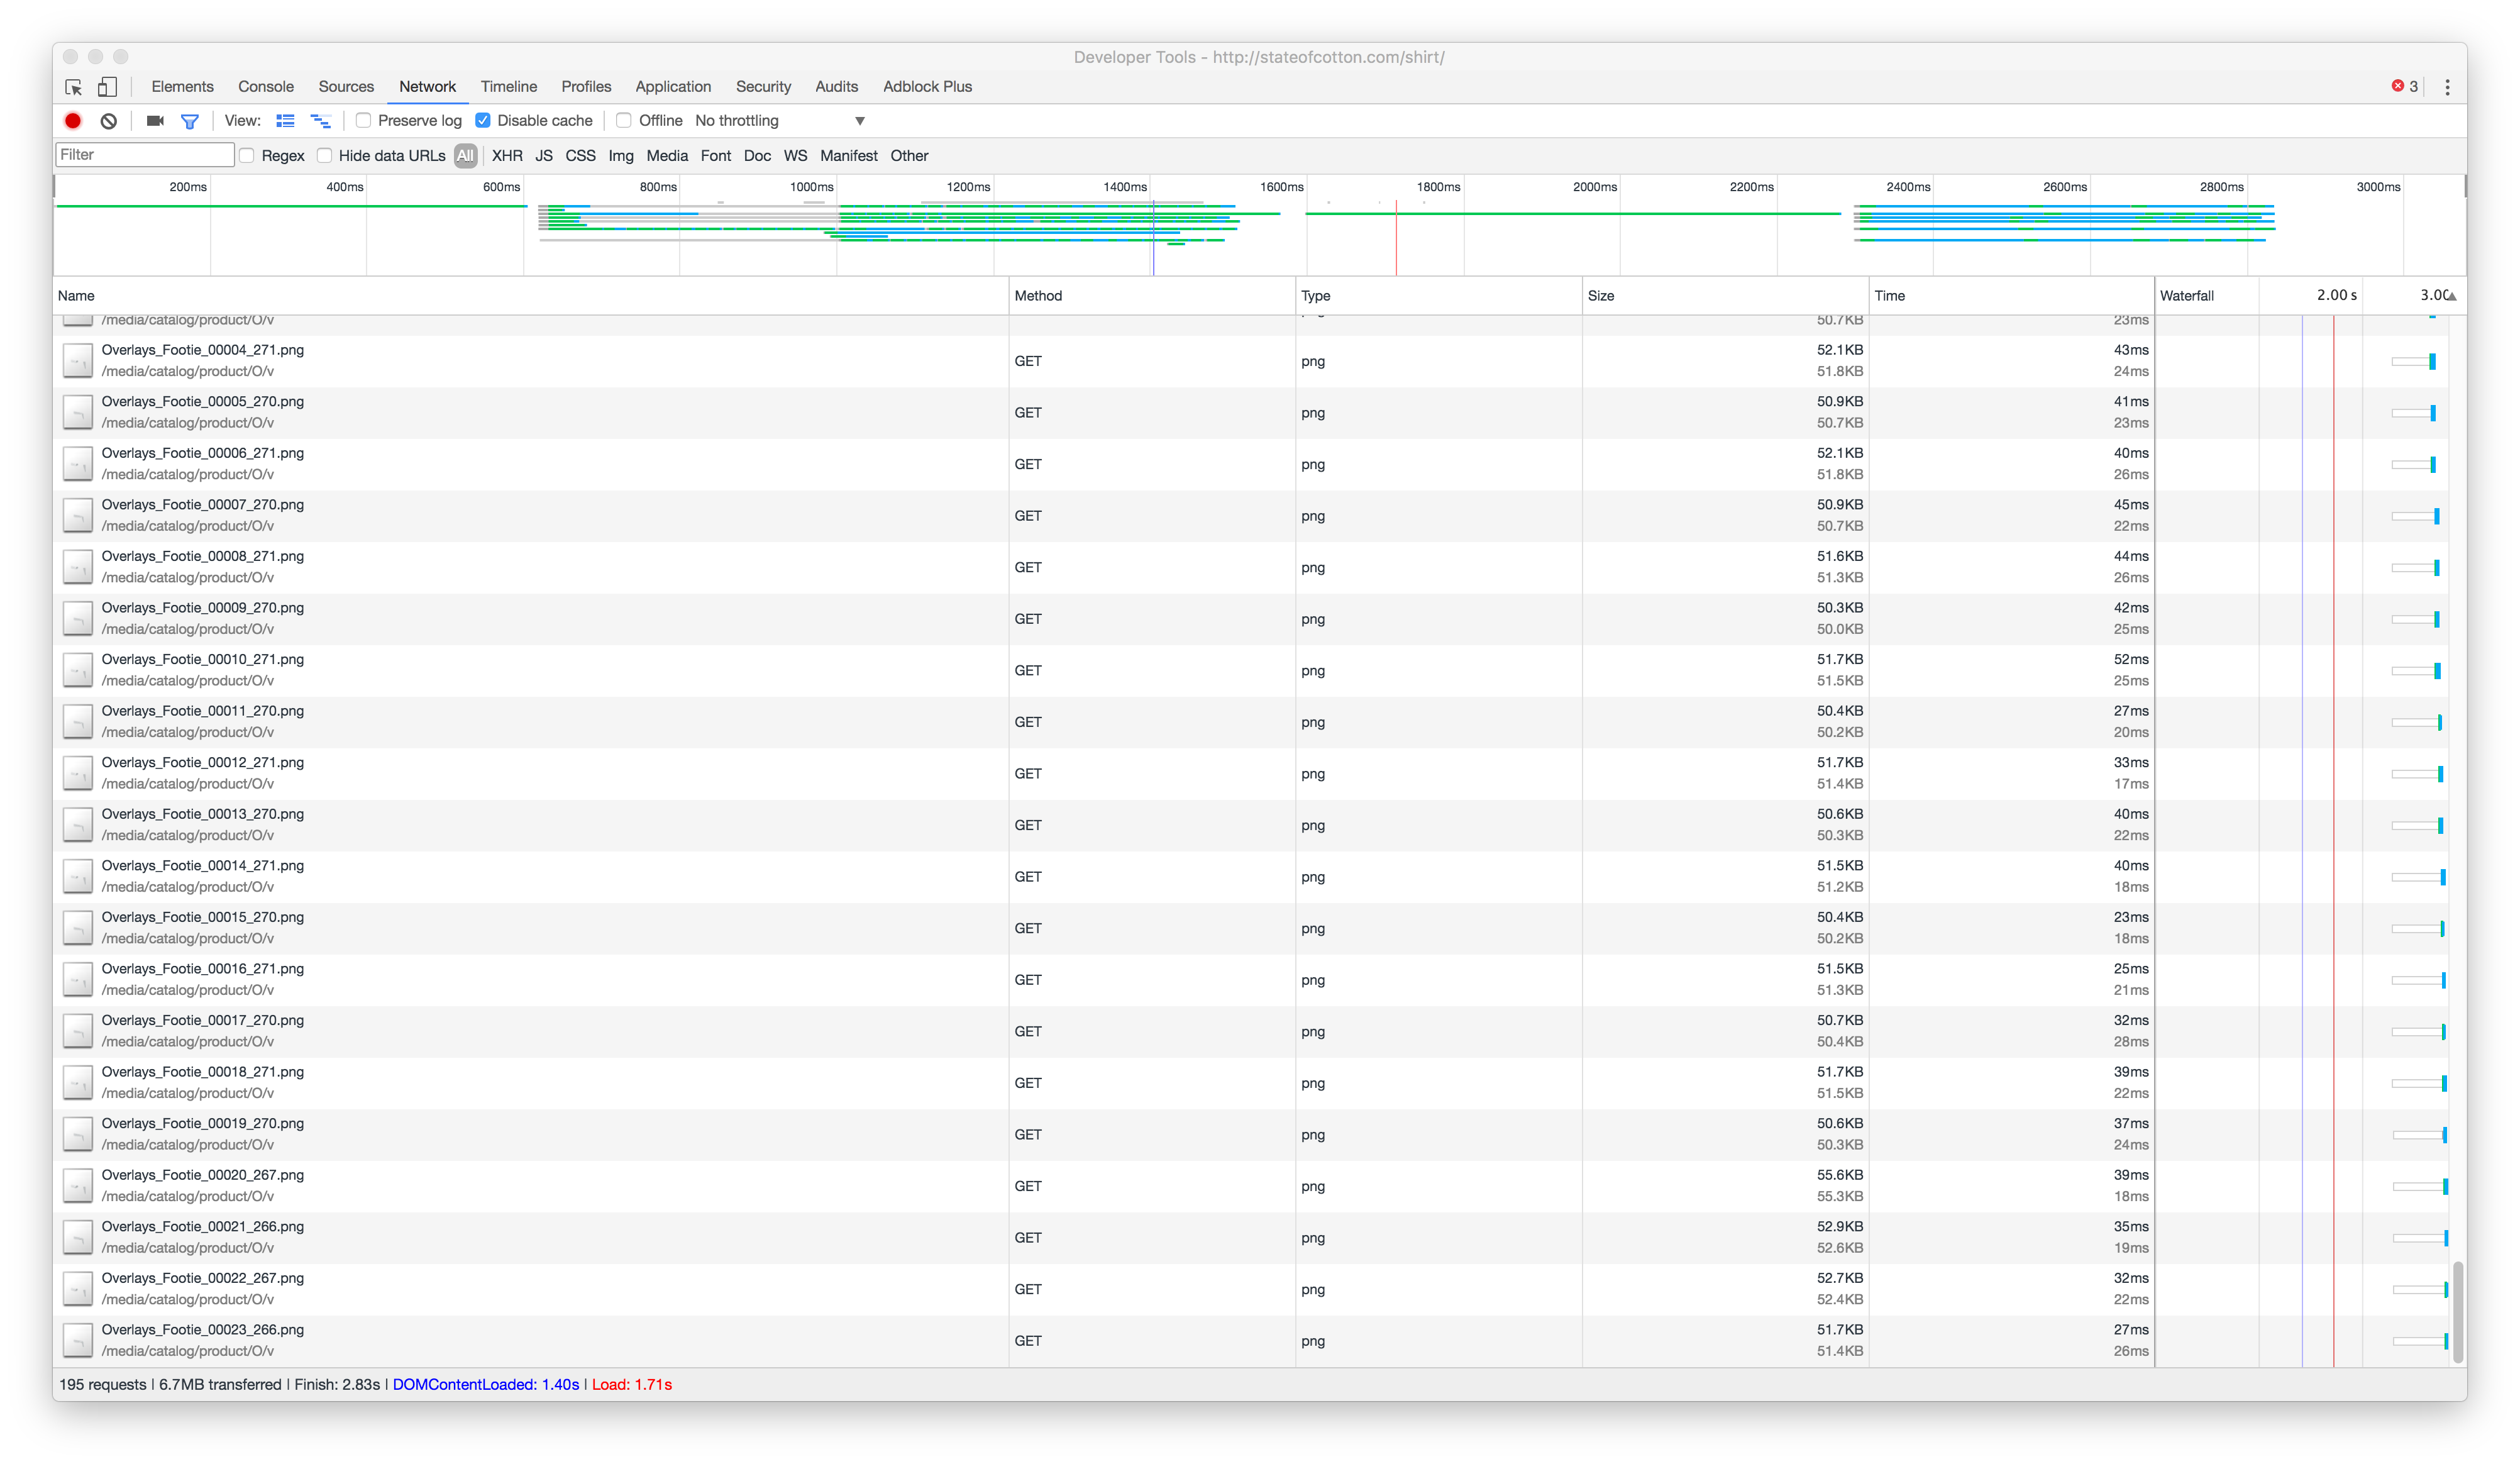
\includegraphics[width=15cm]{images/initialLoad}
\caption{Initial Page Load SlimFitted Configurator}
\label{attachment:initialLoadSlimFitted}
\end{figure}

\begin{figure}
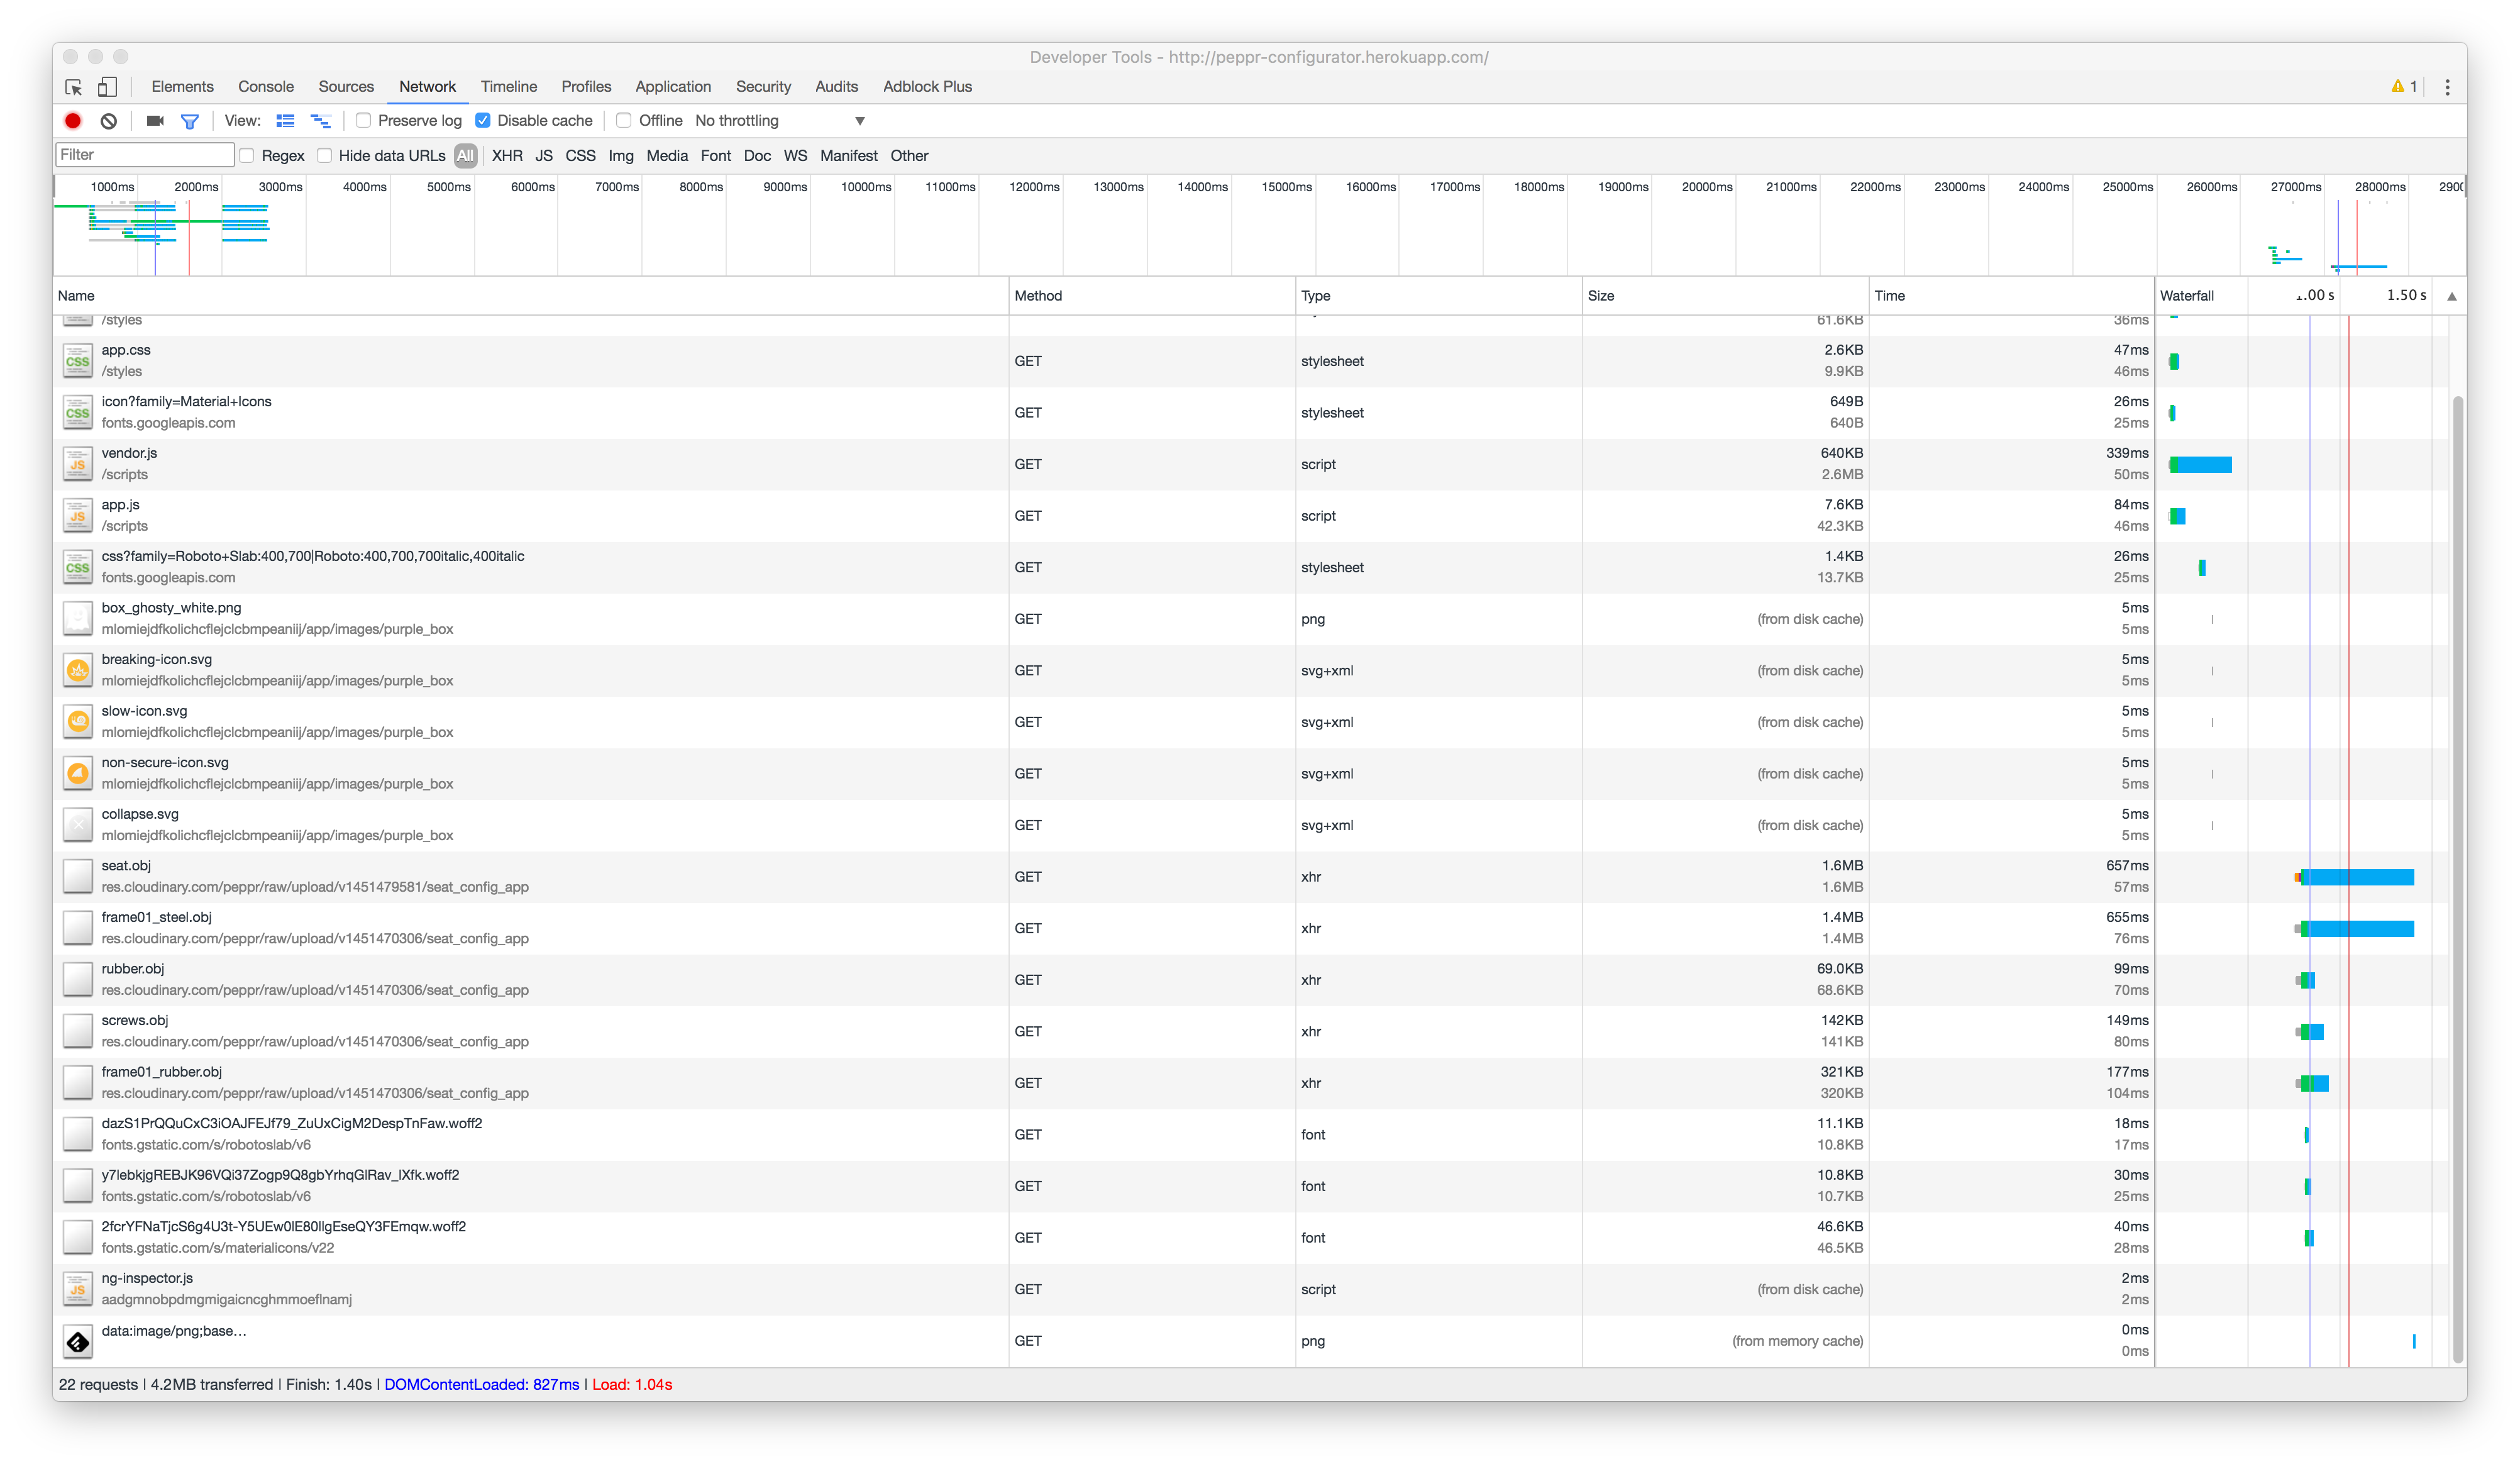
\includegraphics[width=15cm]{images/initialLoadWebgl}
\caption{Initial Page Load WebGL Configurator}
\label{attachment:initialLoadWebGL}
\end{figure}

\clearpage

\begin{figure}
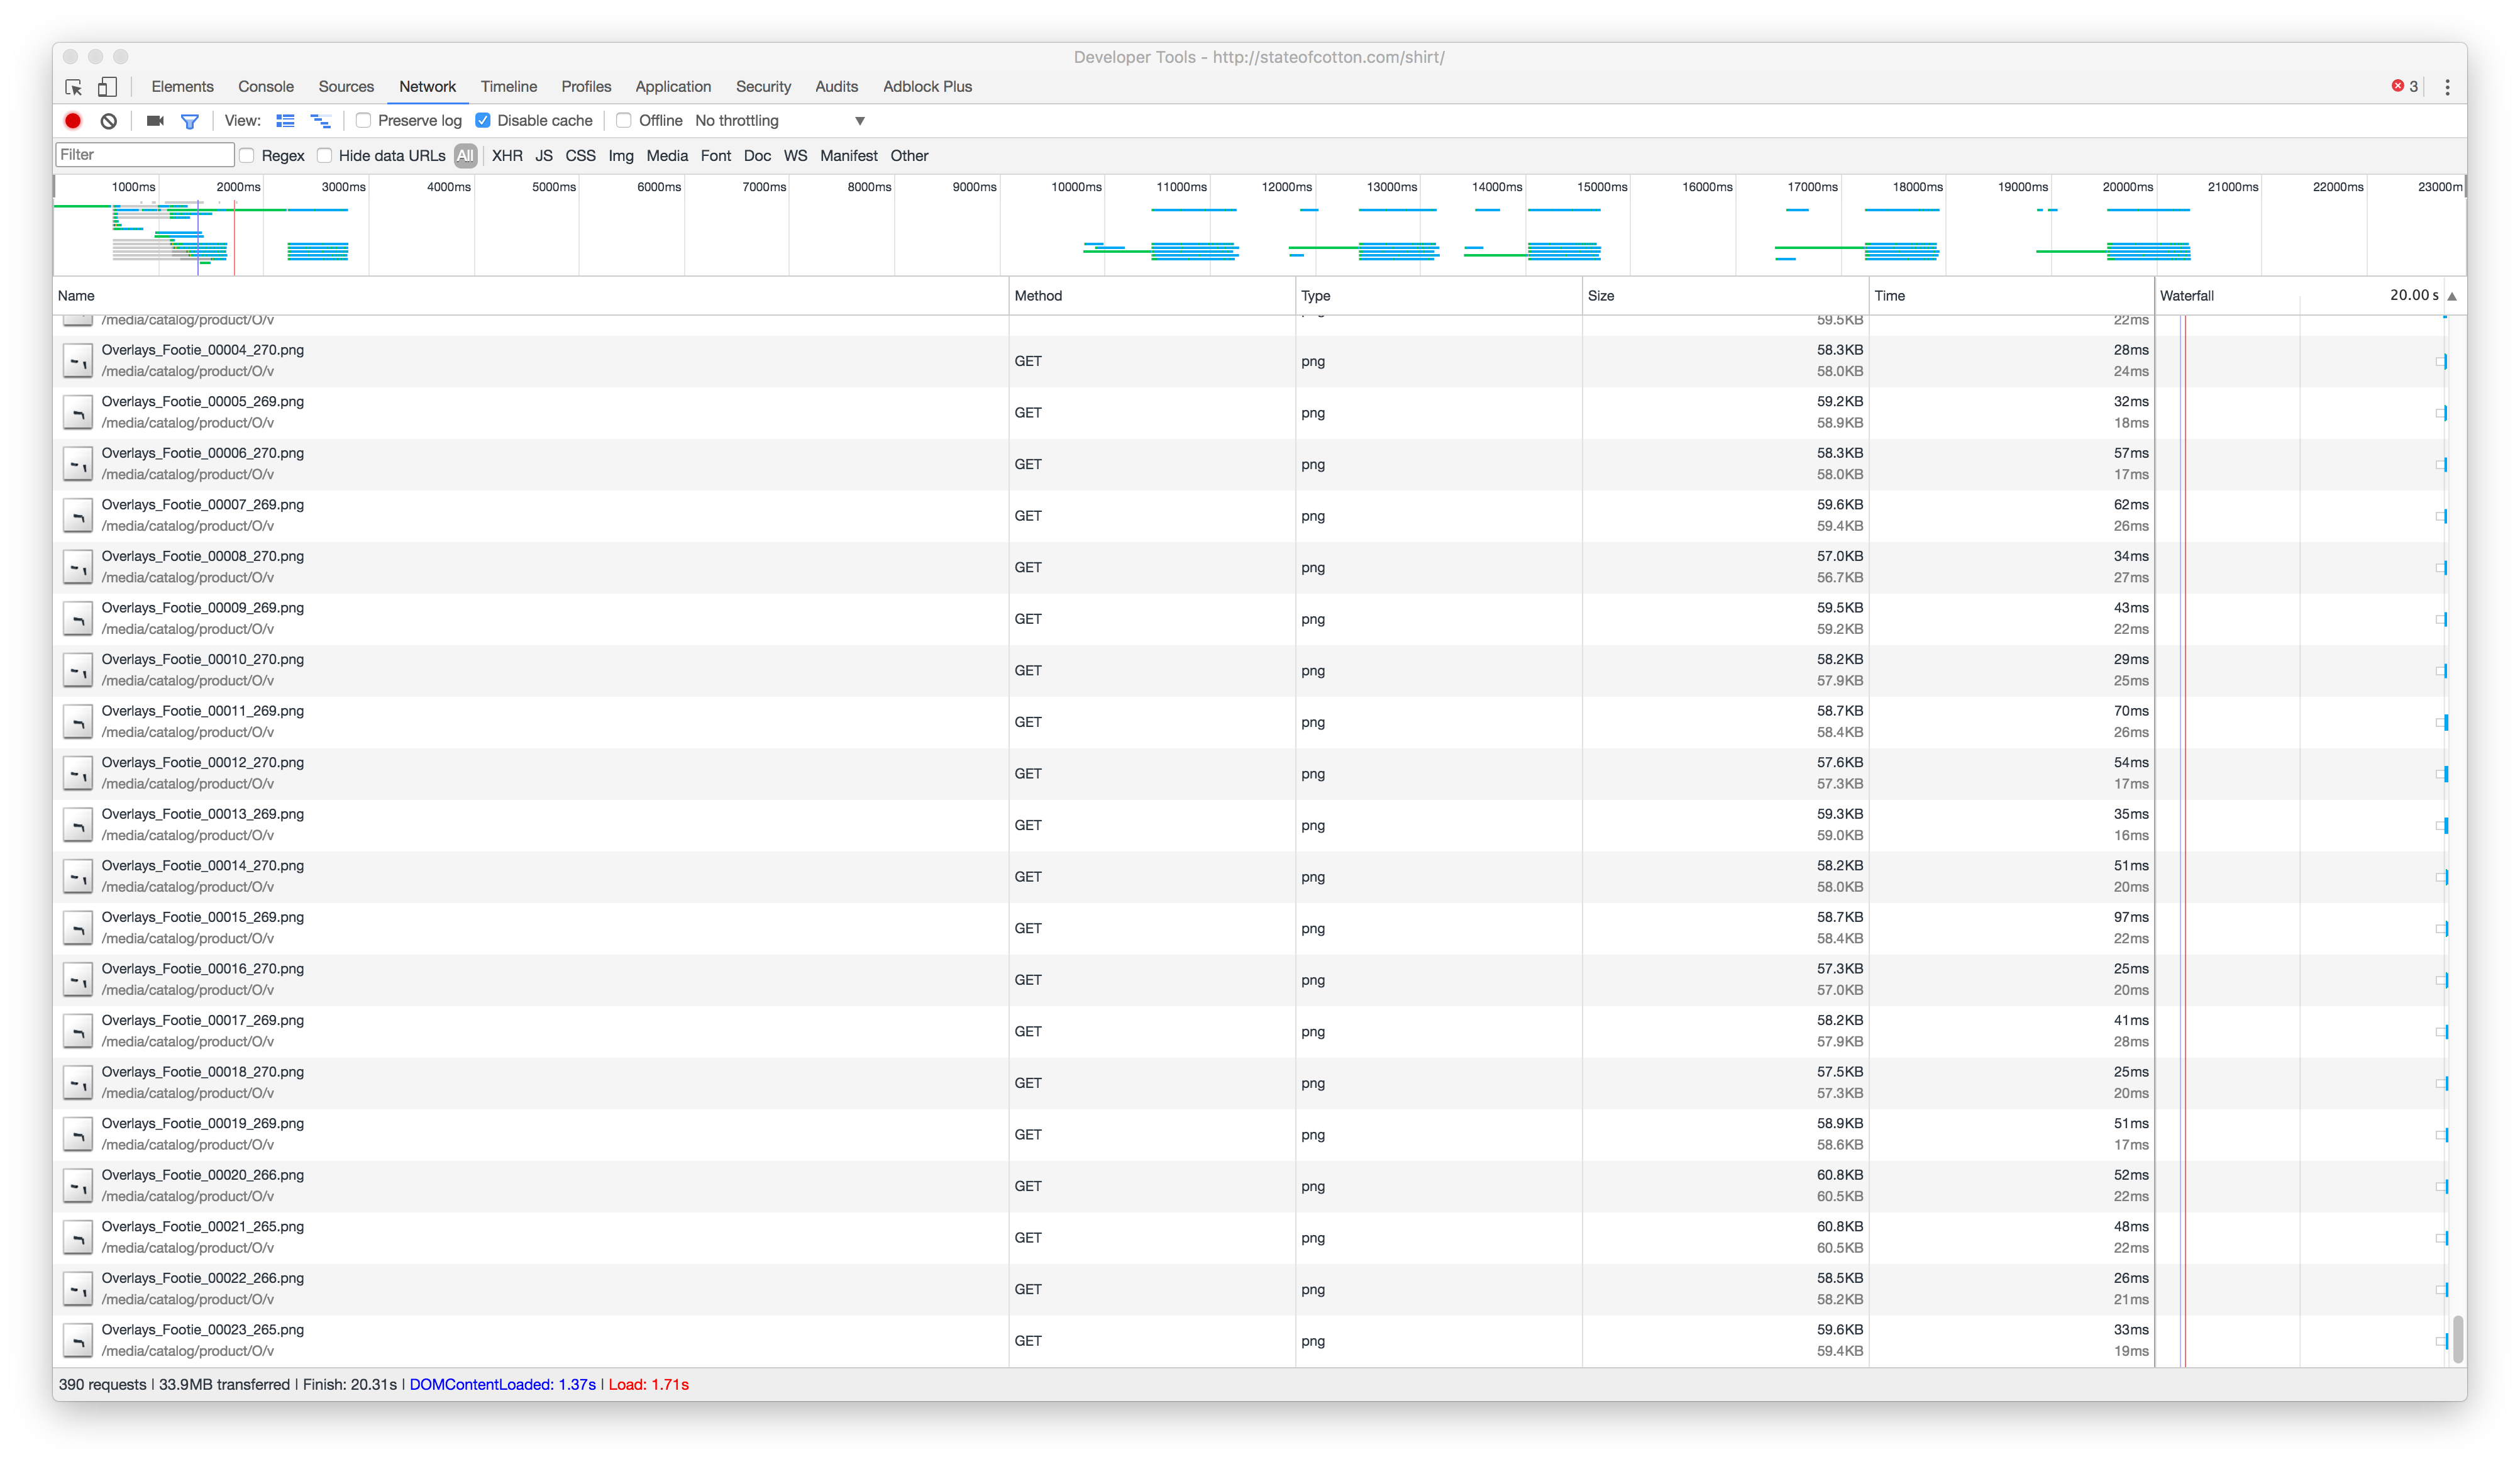
\includegraphics[width=15cm]{images/5differentColours}
\caption{Page Load 5 colours Slimfitted}
\label{attachment:fiveColoursSlimFitted}
\end{figure}

\begin{figure}
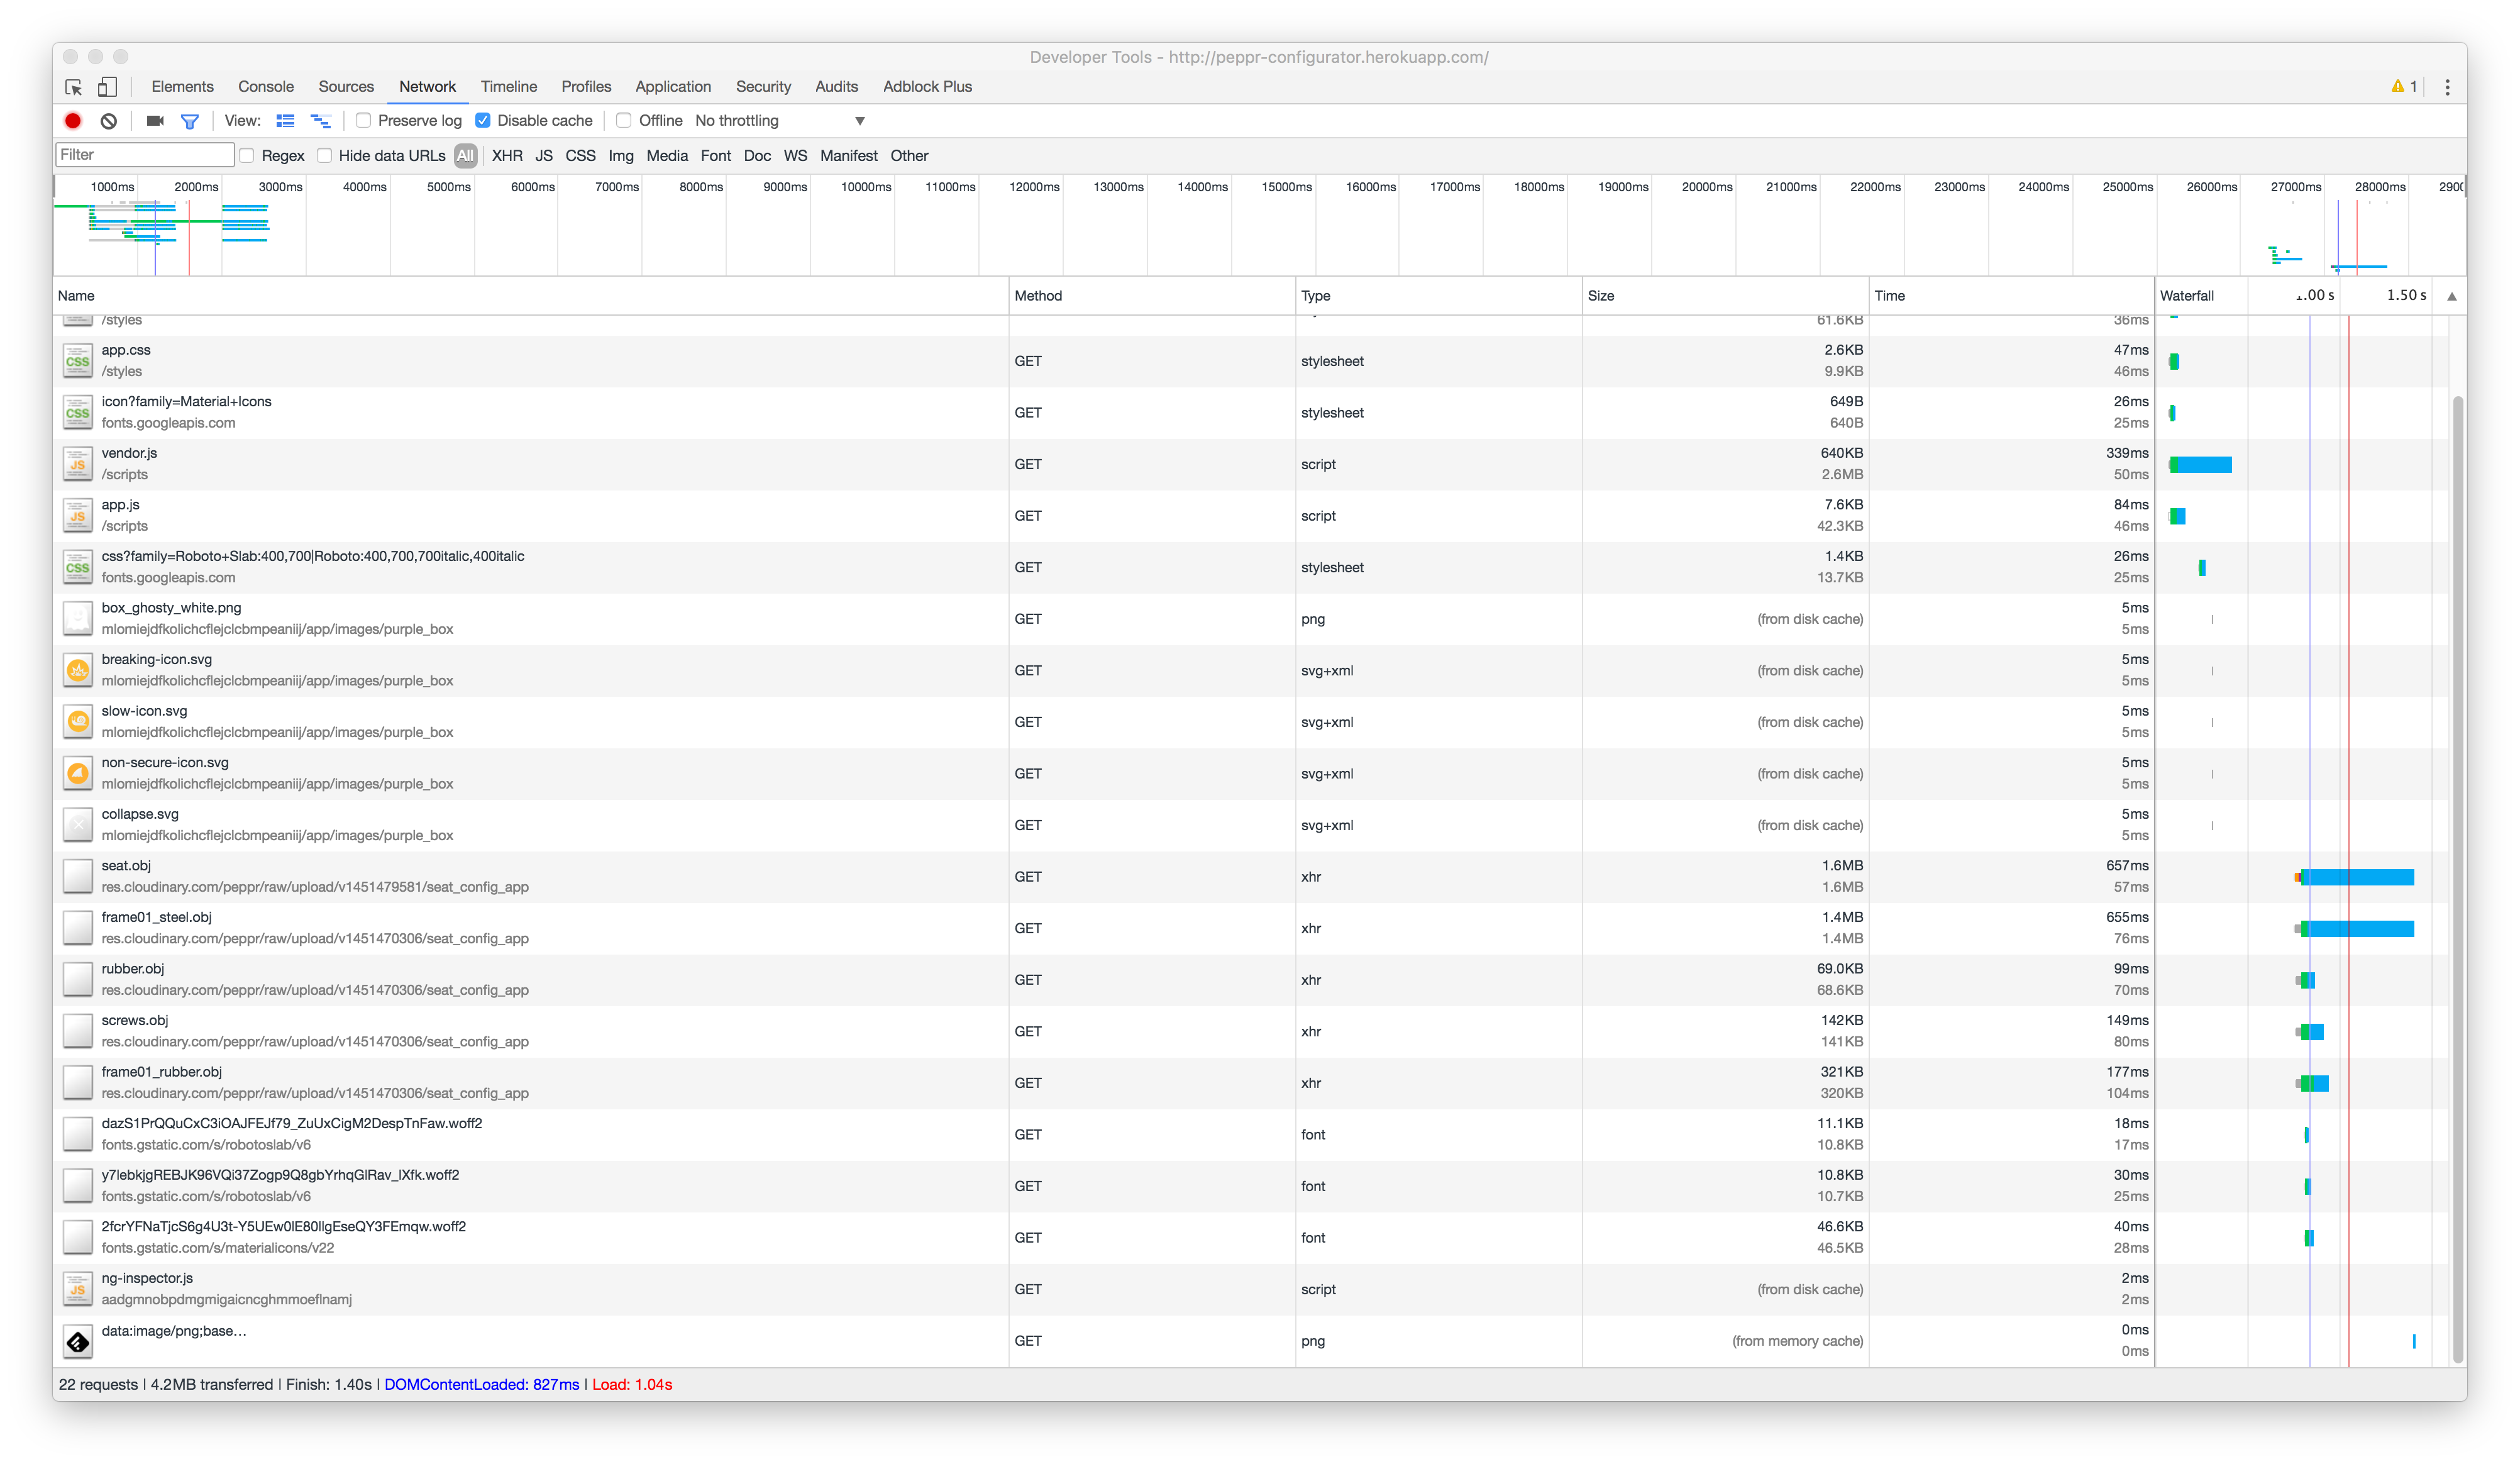
\includegraphics[width=15cm]{images/5differentColoursWebGL}
\caption{Page Load 5 colours WebGL}
\label{attachment:fiveColoursWebgl}
\end{figure}

\clearpage

\begin{figure}
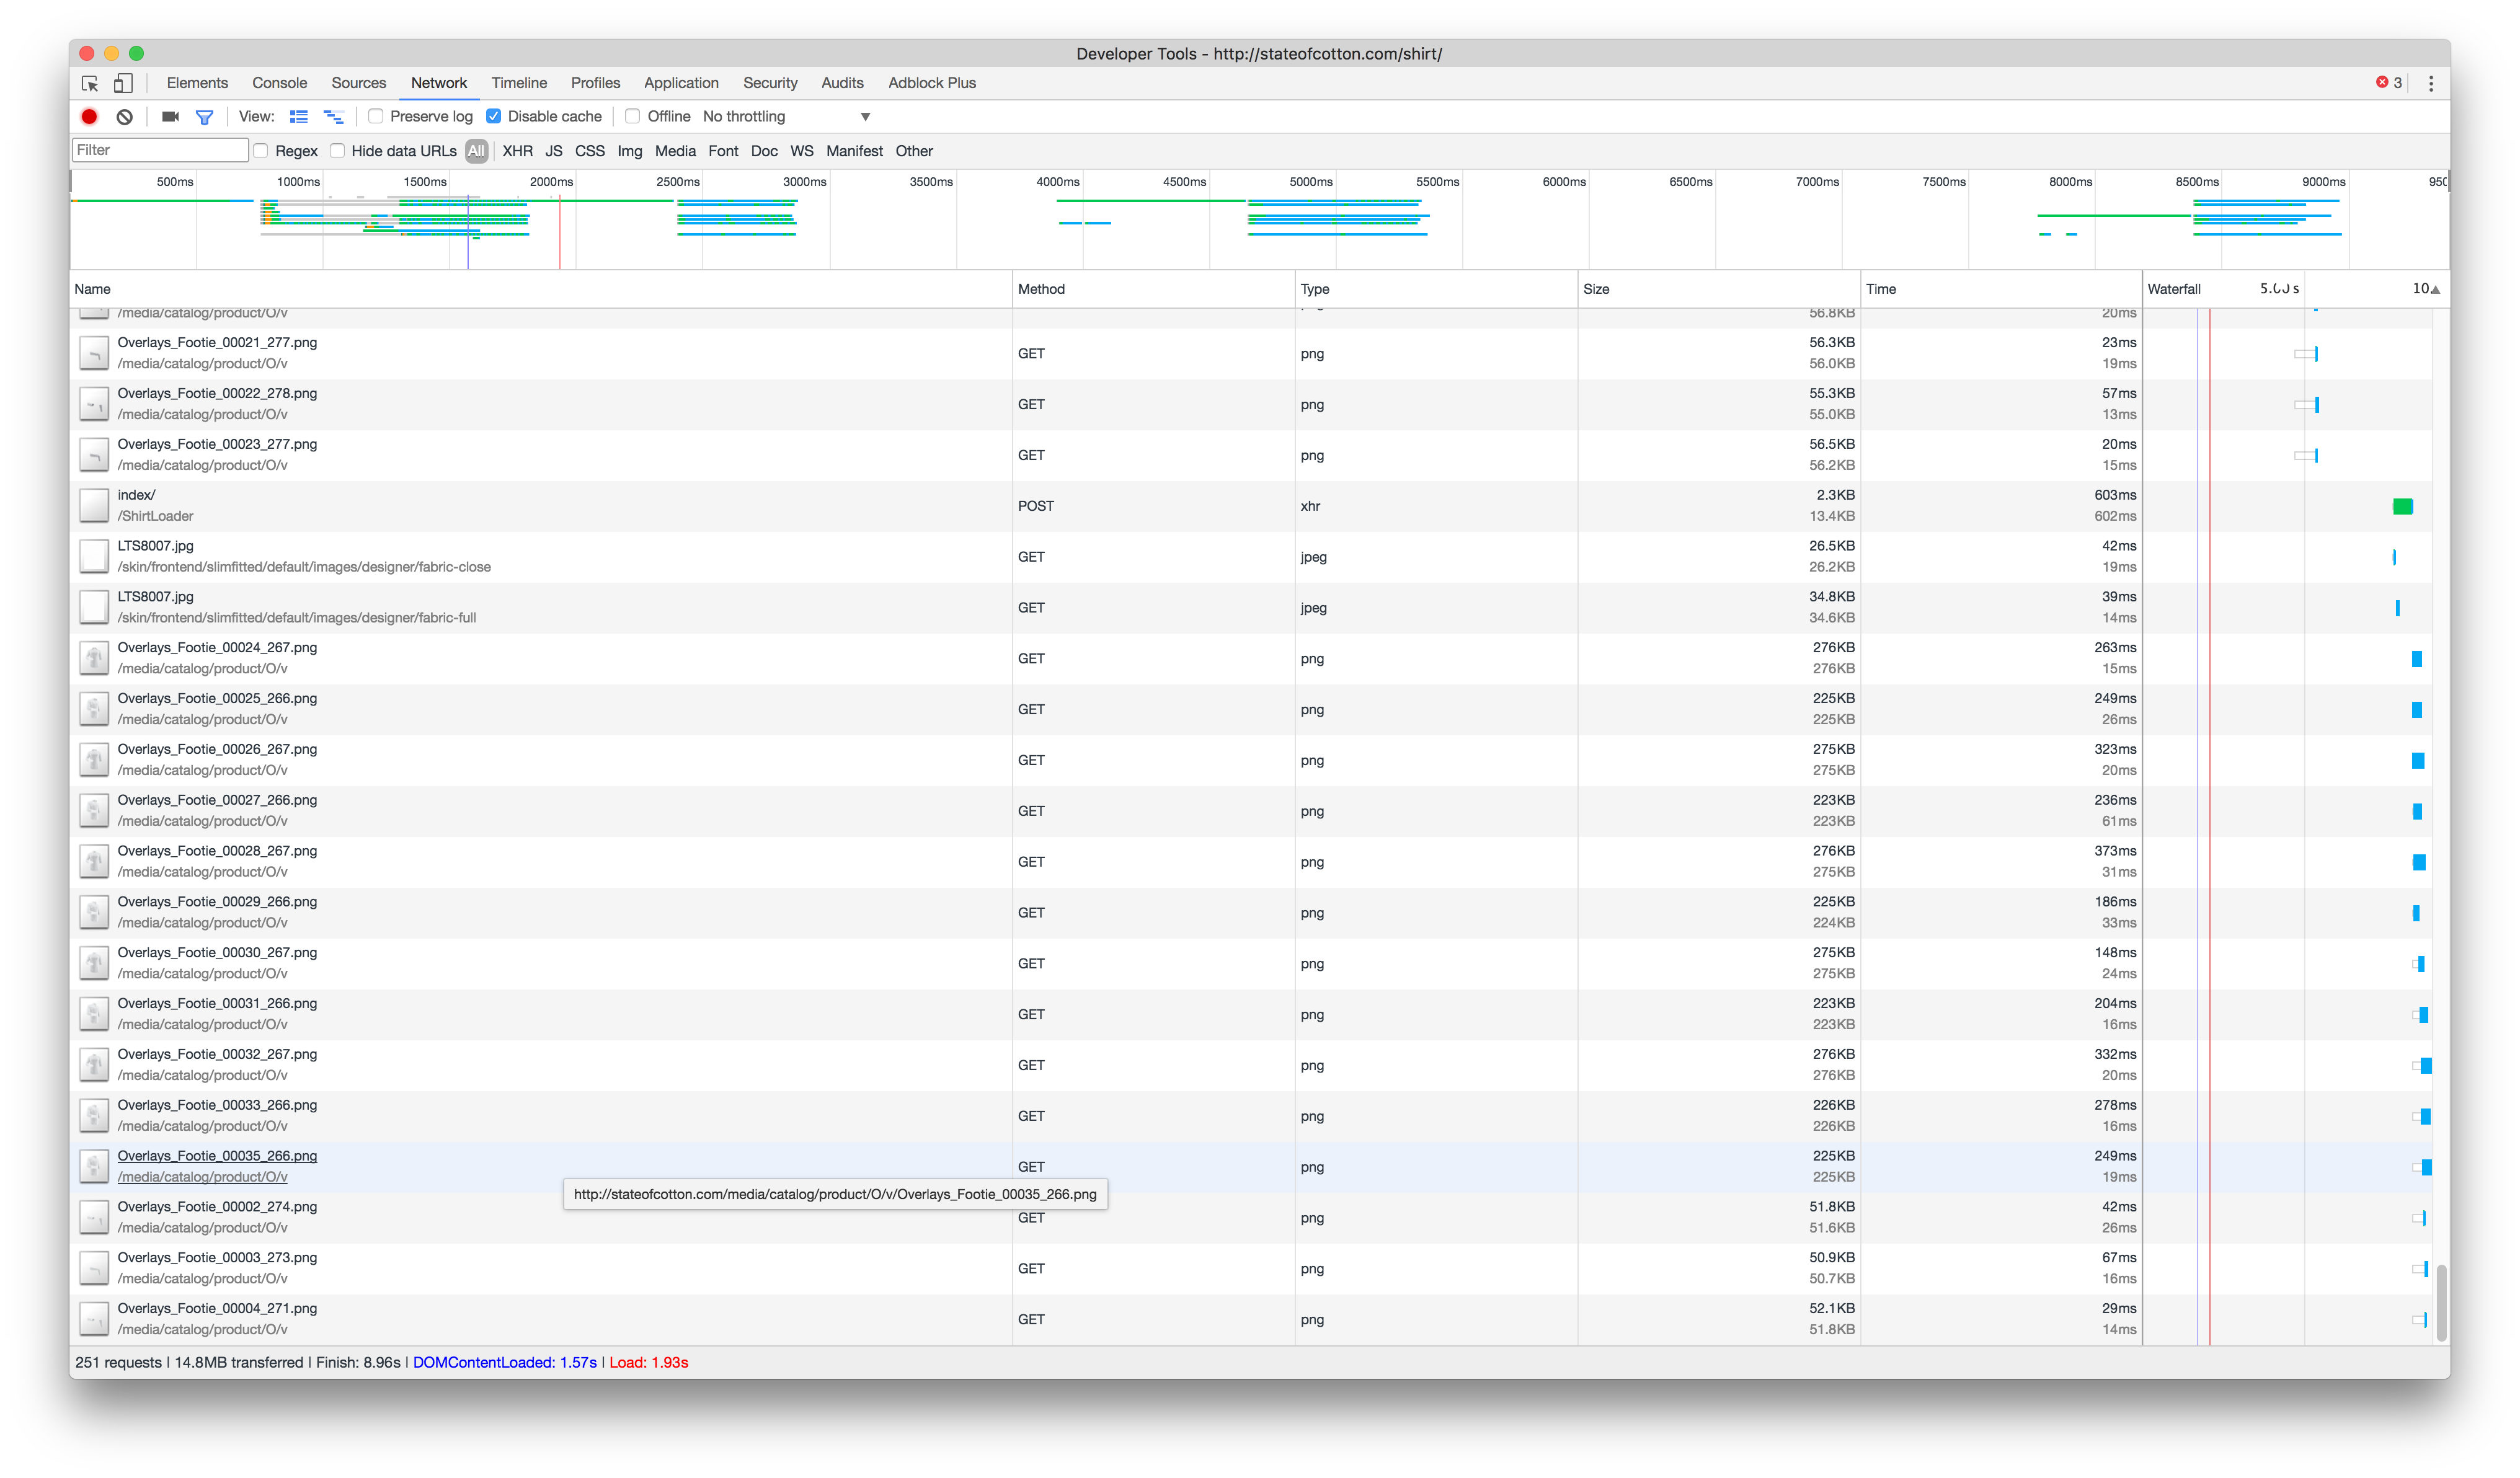
\includegraphics[width=15cm]{images/2coloursSwap}
\caption{Page Load 2 colour swap SlimFitted}
\label{attachment:twoColourSwap}
\end{figure}

\begin{figure}
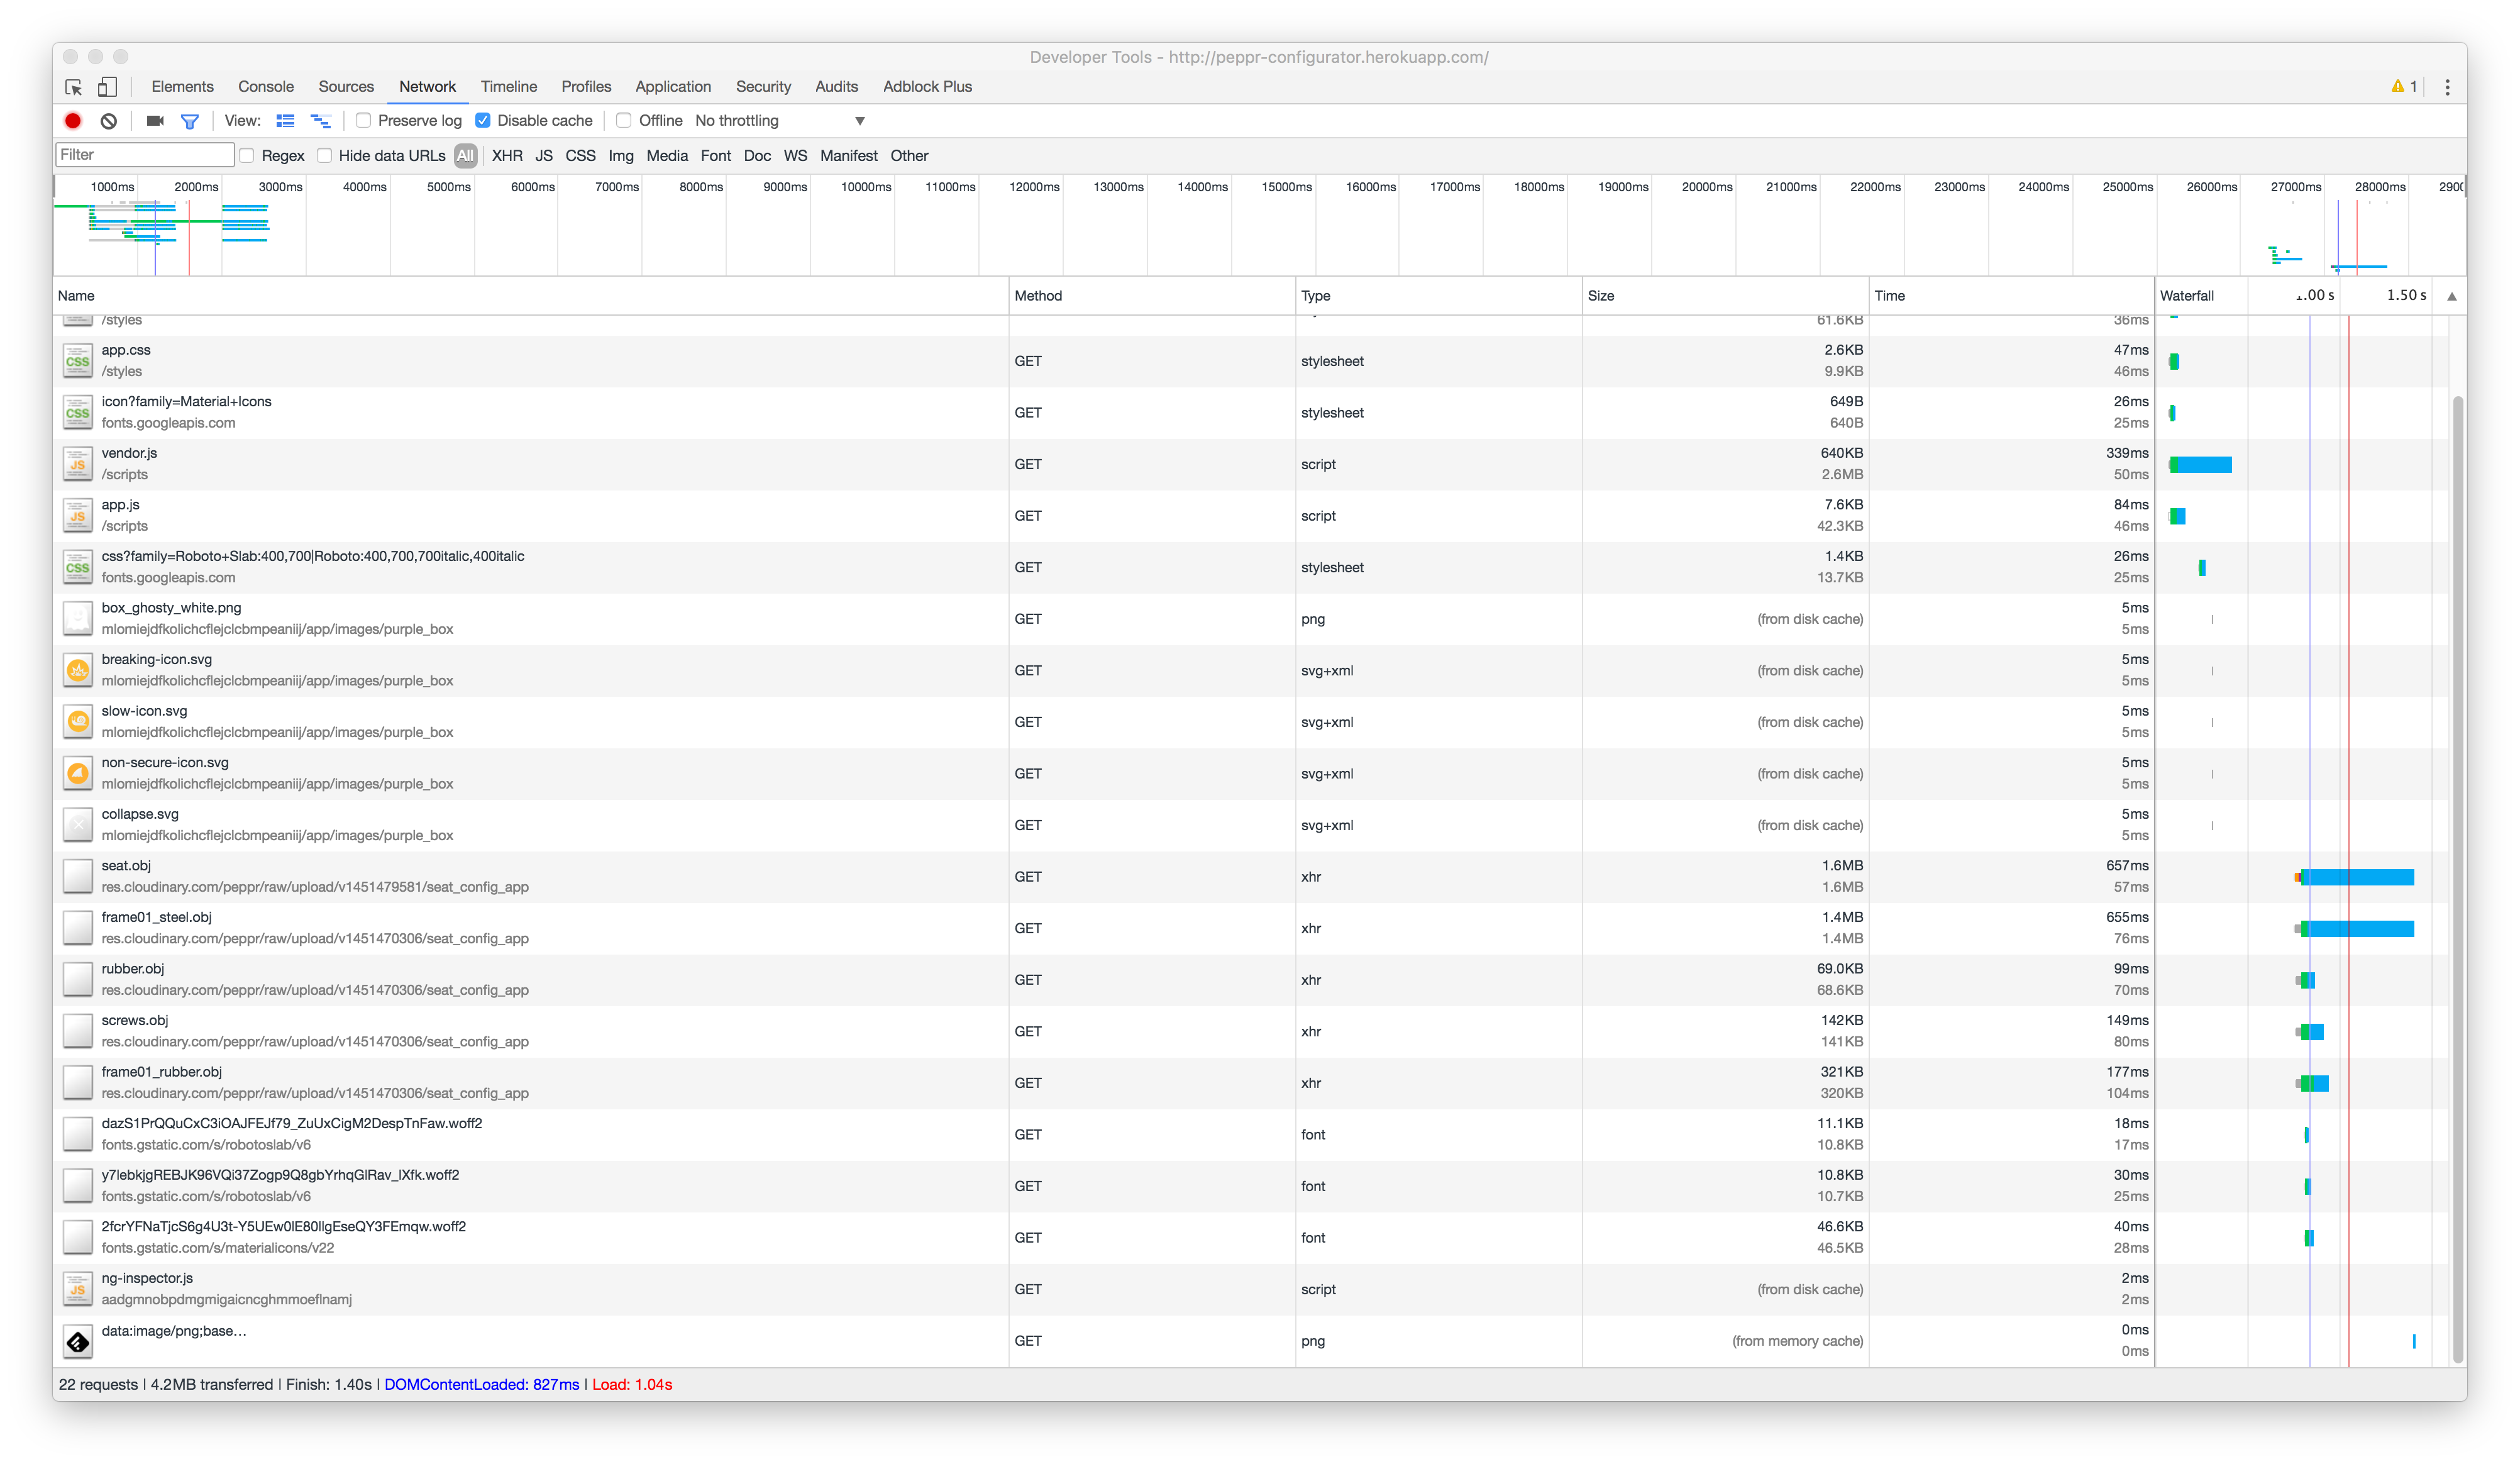
\includegraphics[width=15cm]{images/2ColoursSwapWebGL}
\caption{Page Load 2 colour swap WebGL}
\label{attachment:2ColoursSwapWebGL}
\end{figure}

\clearpage

\begin{figure}
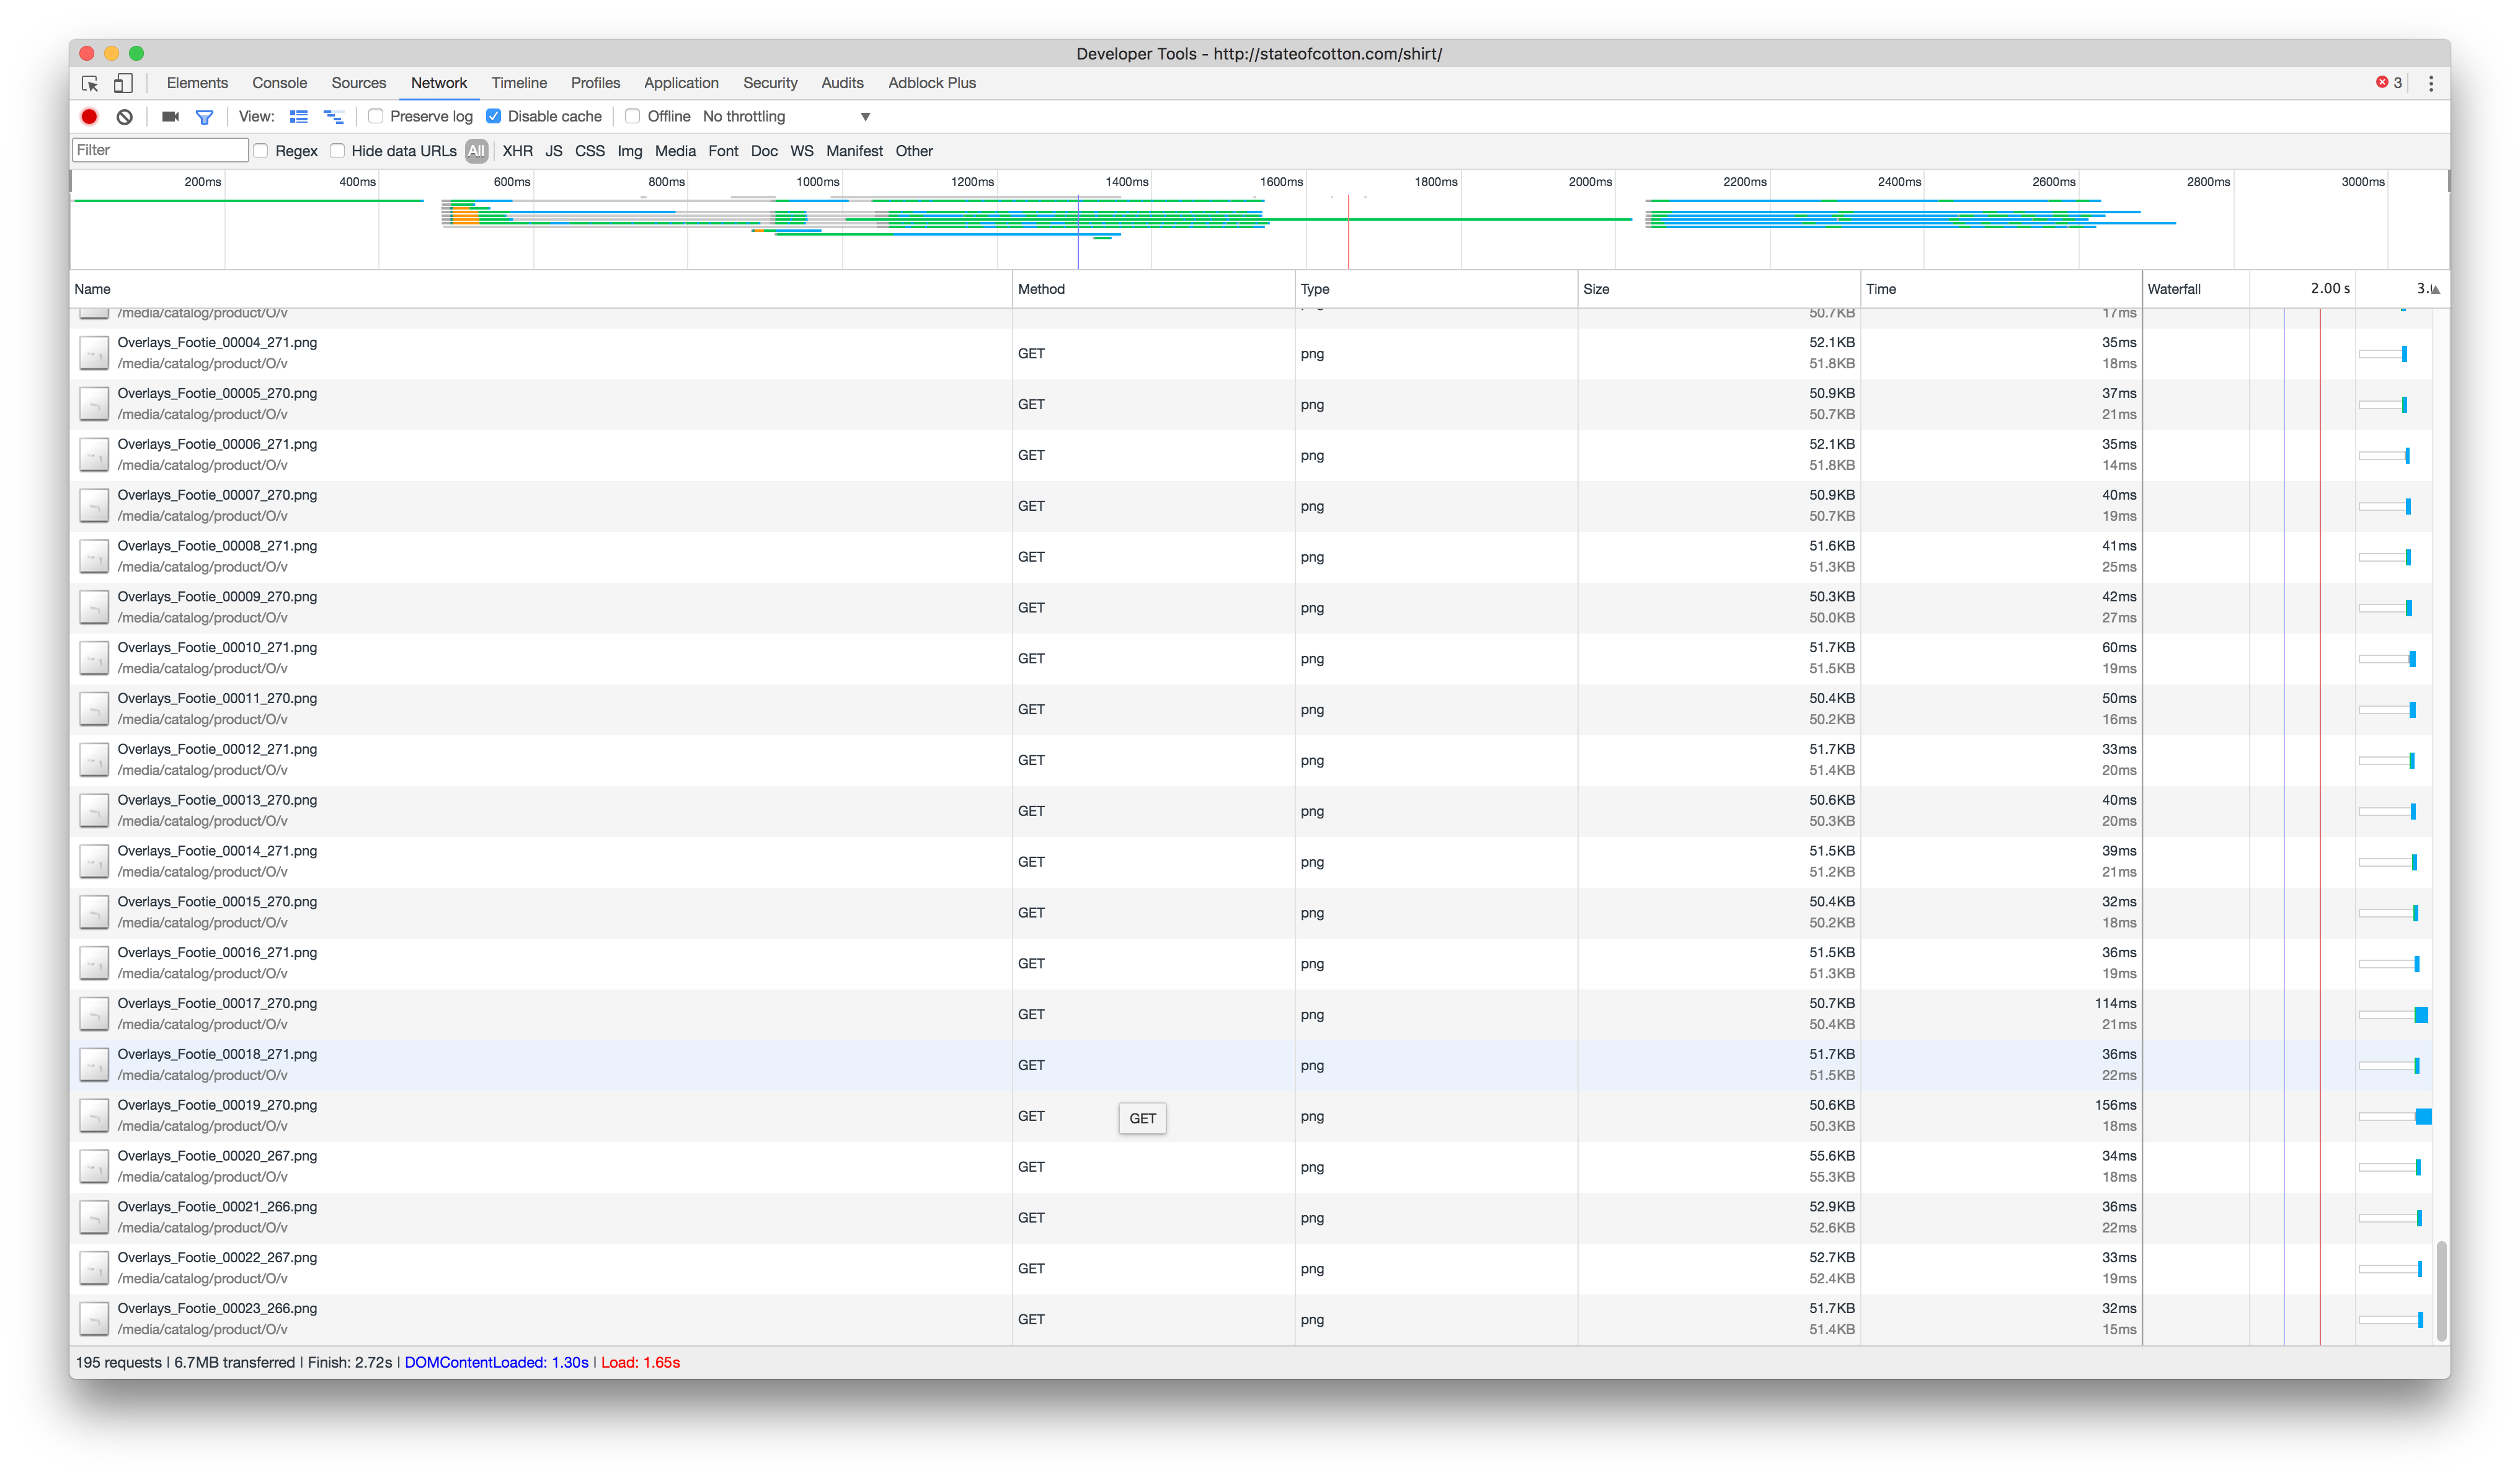
\includegraphics[width=15cm]{images/2differentComponents}
\caption{Page Load 2 differen component SlimFitted}
\label{attachment:2differentComponents}
\end{figure}

\begin{figure}
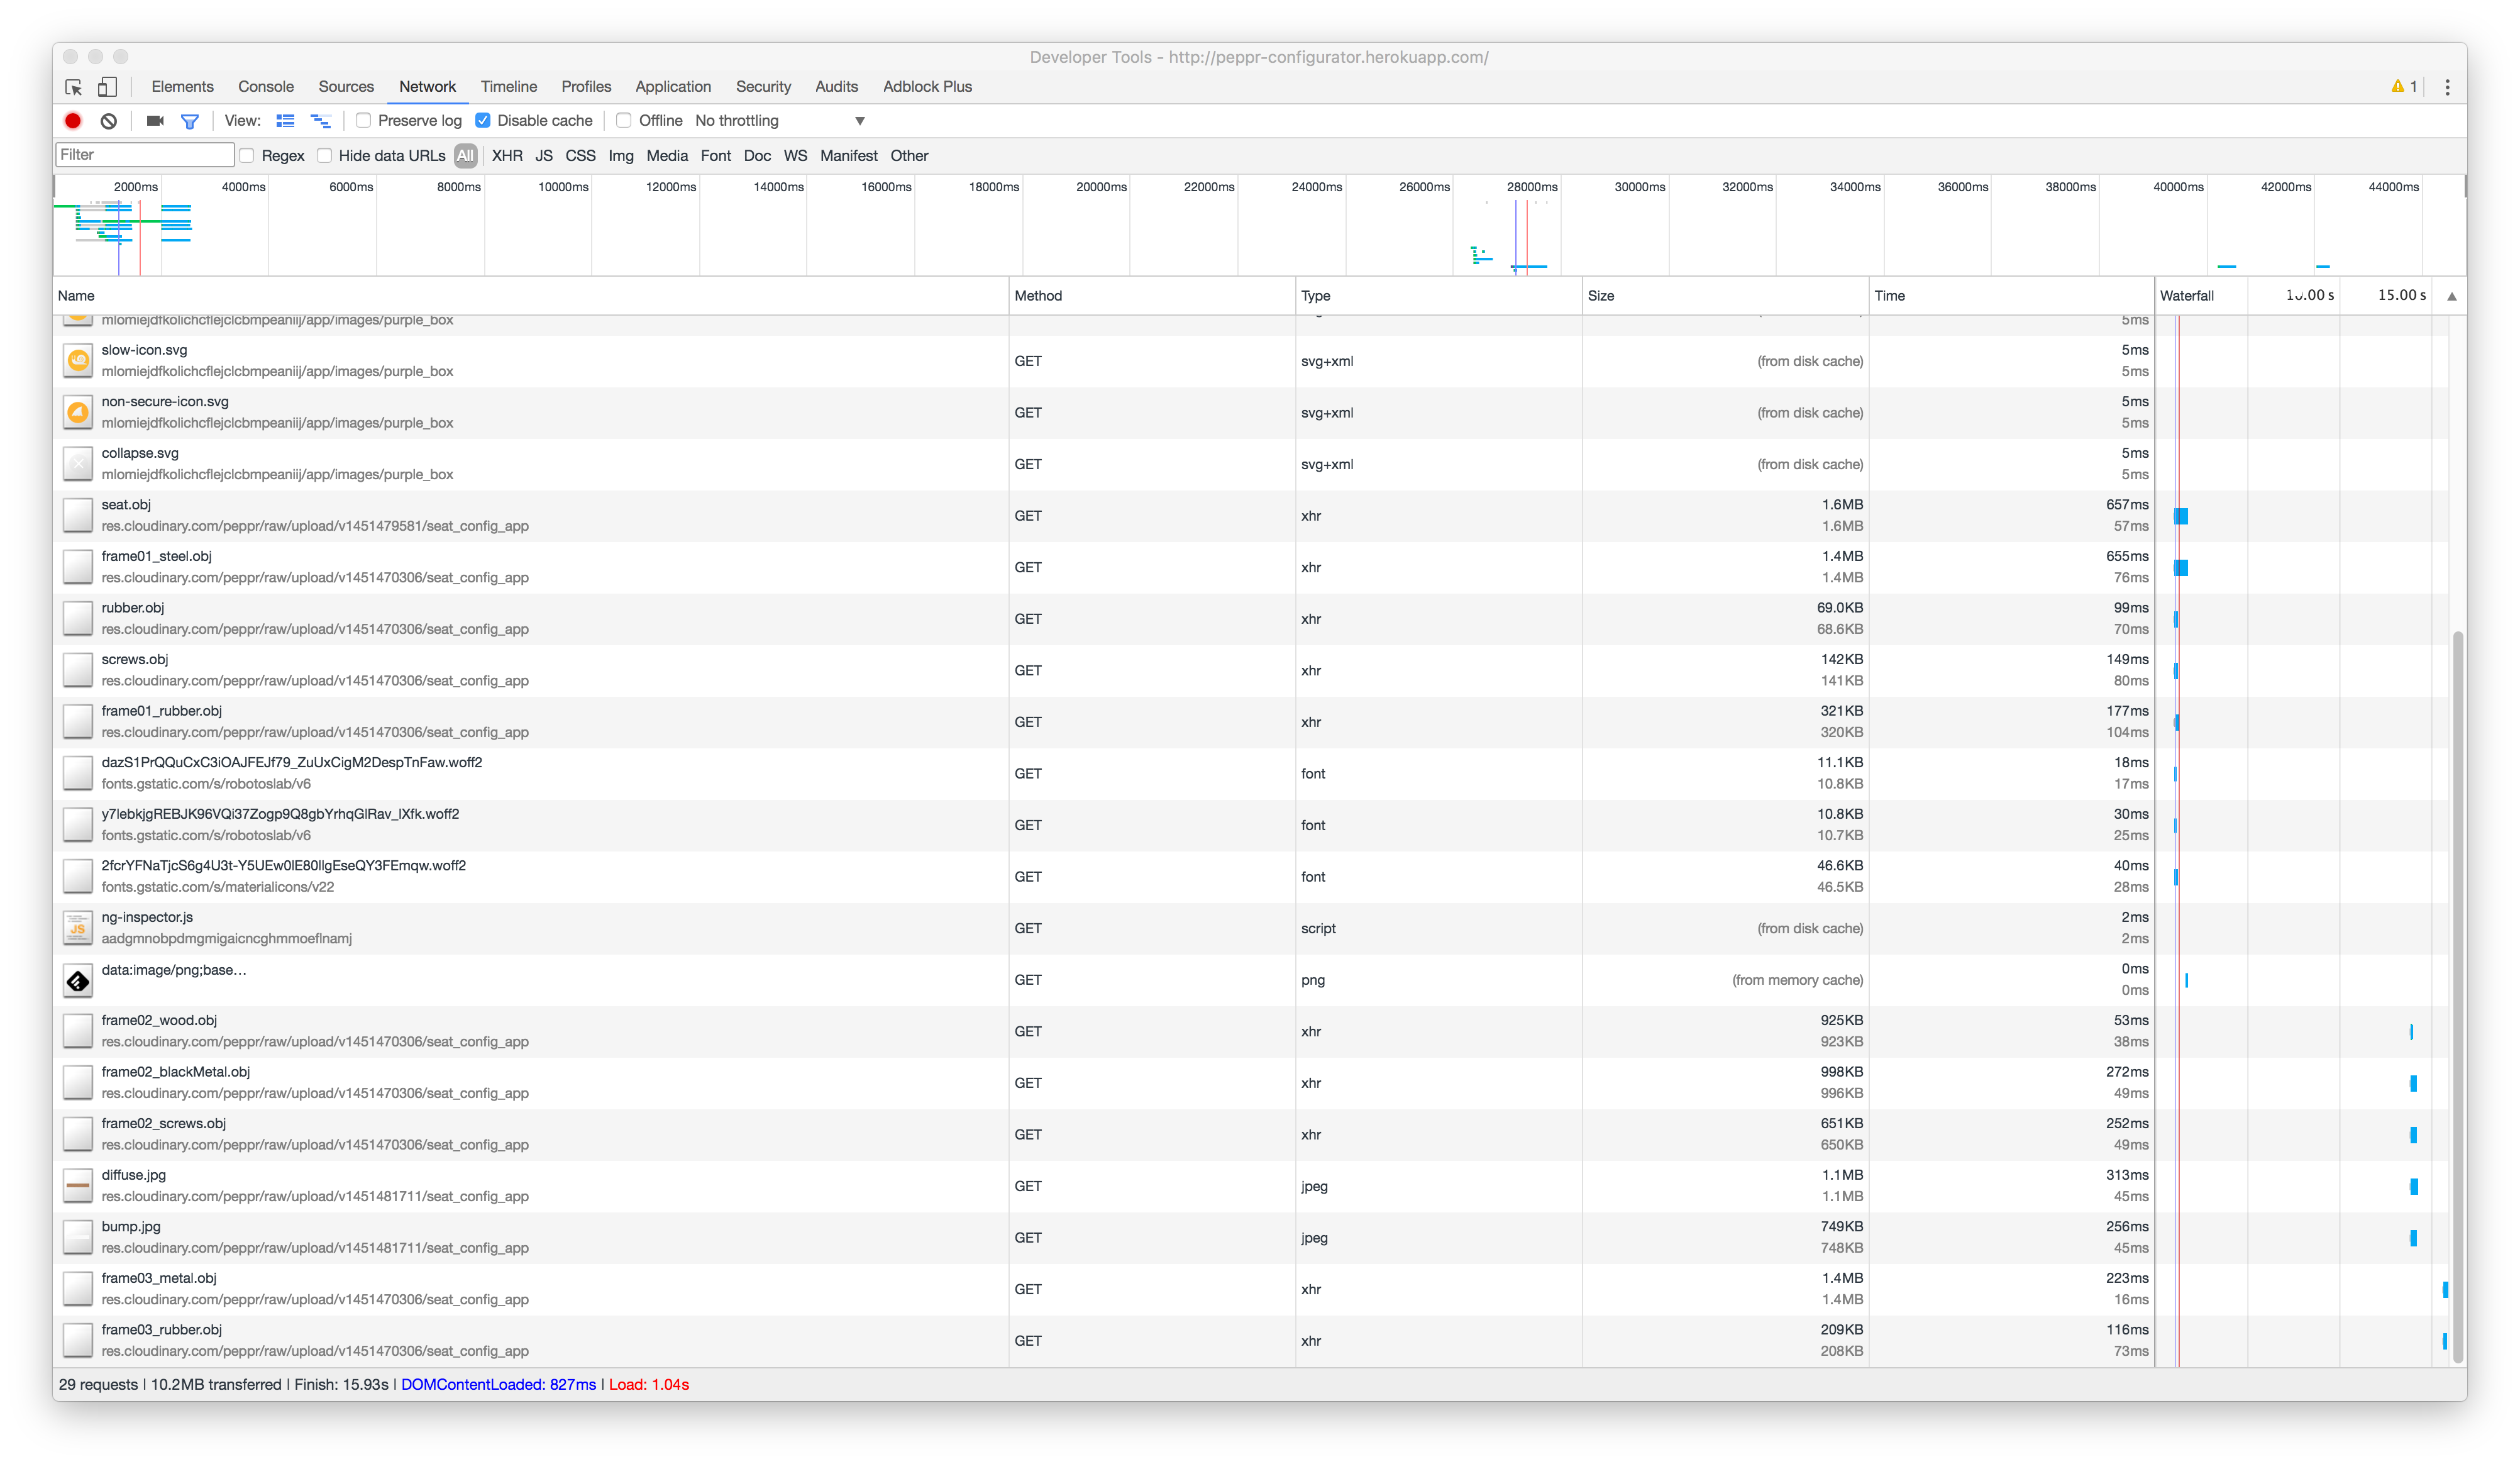
\includegraphics[width=15cm]{images/2differentComponentsWebGL}
\caption{Page Load 2 differen component WebGL}
\label{attachment:2differentComponentsWebGL}
\end{figure}

\clearpage

\begin{figure}
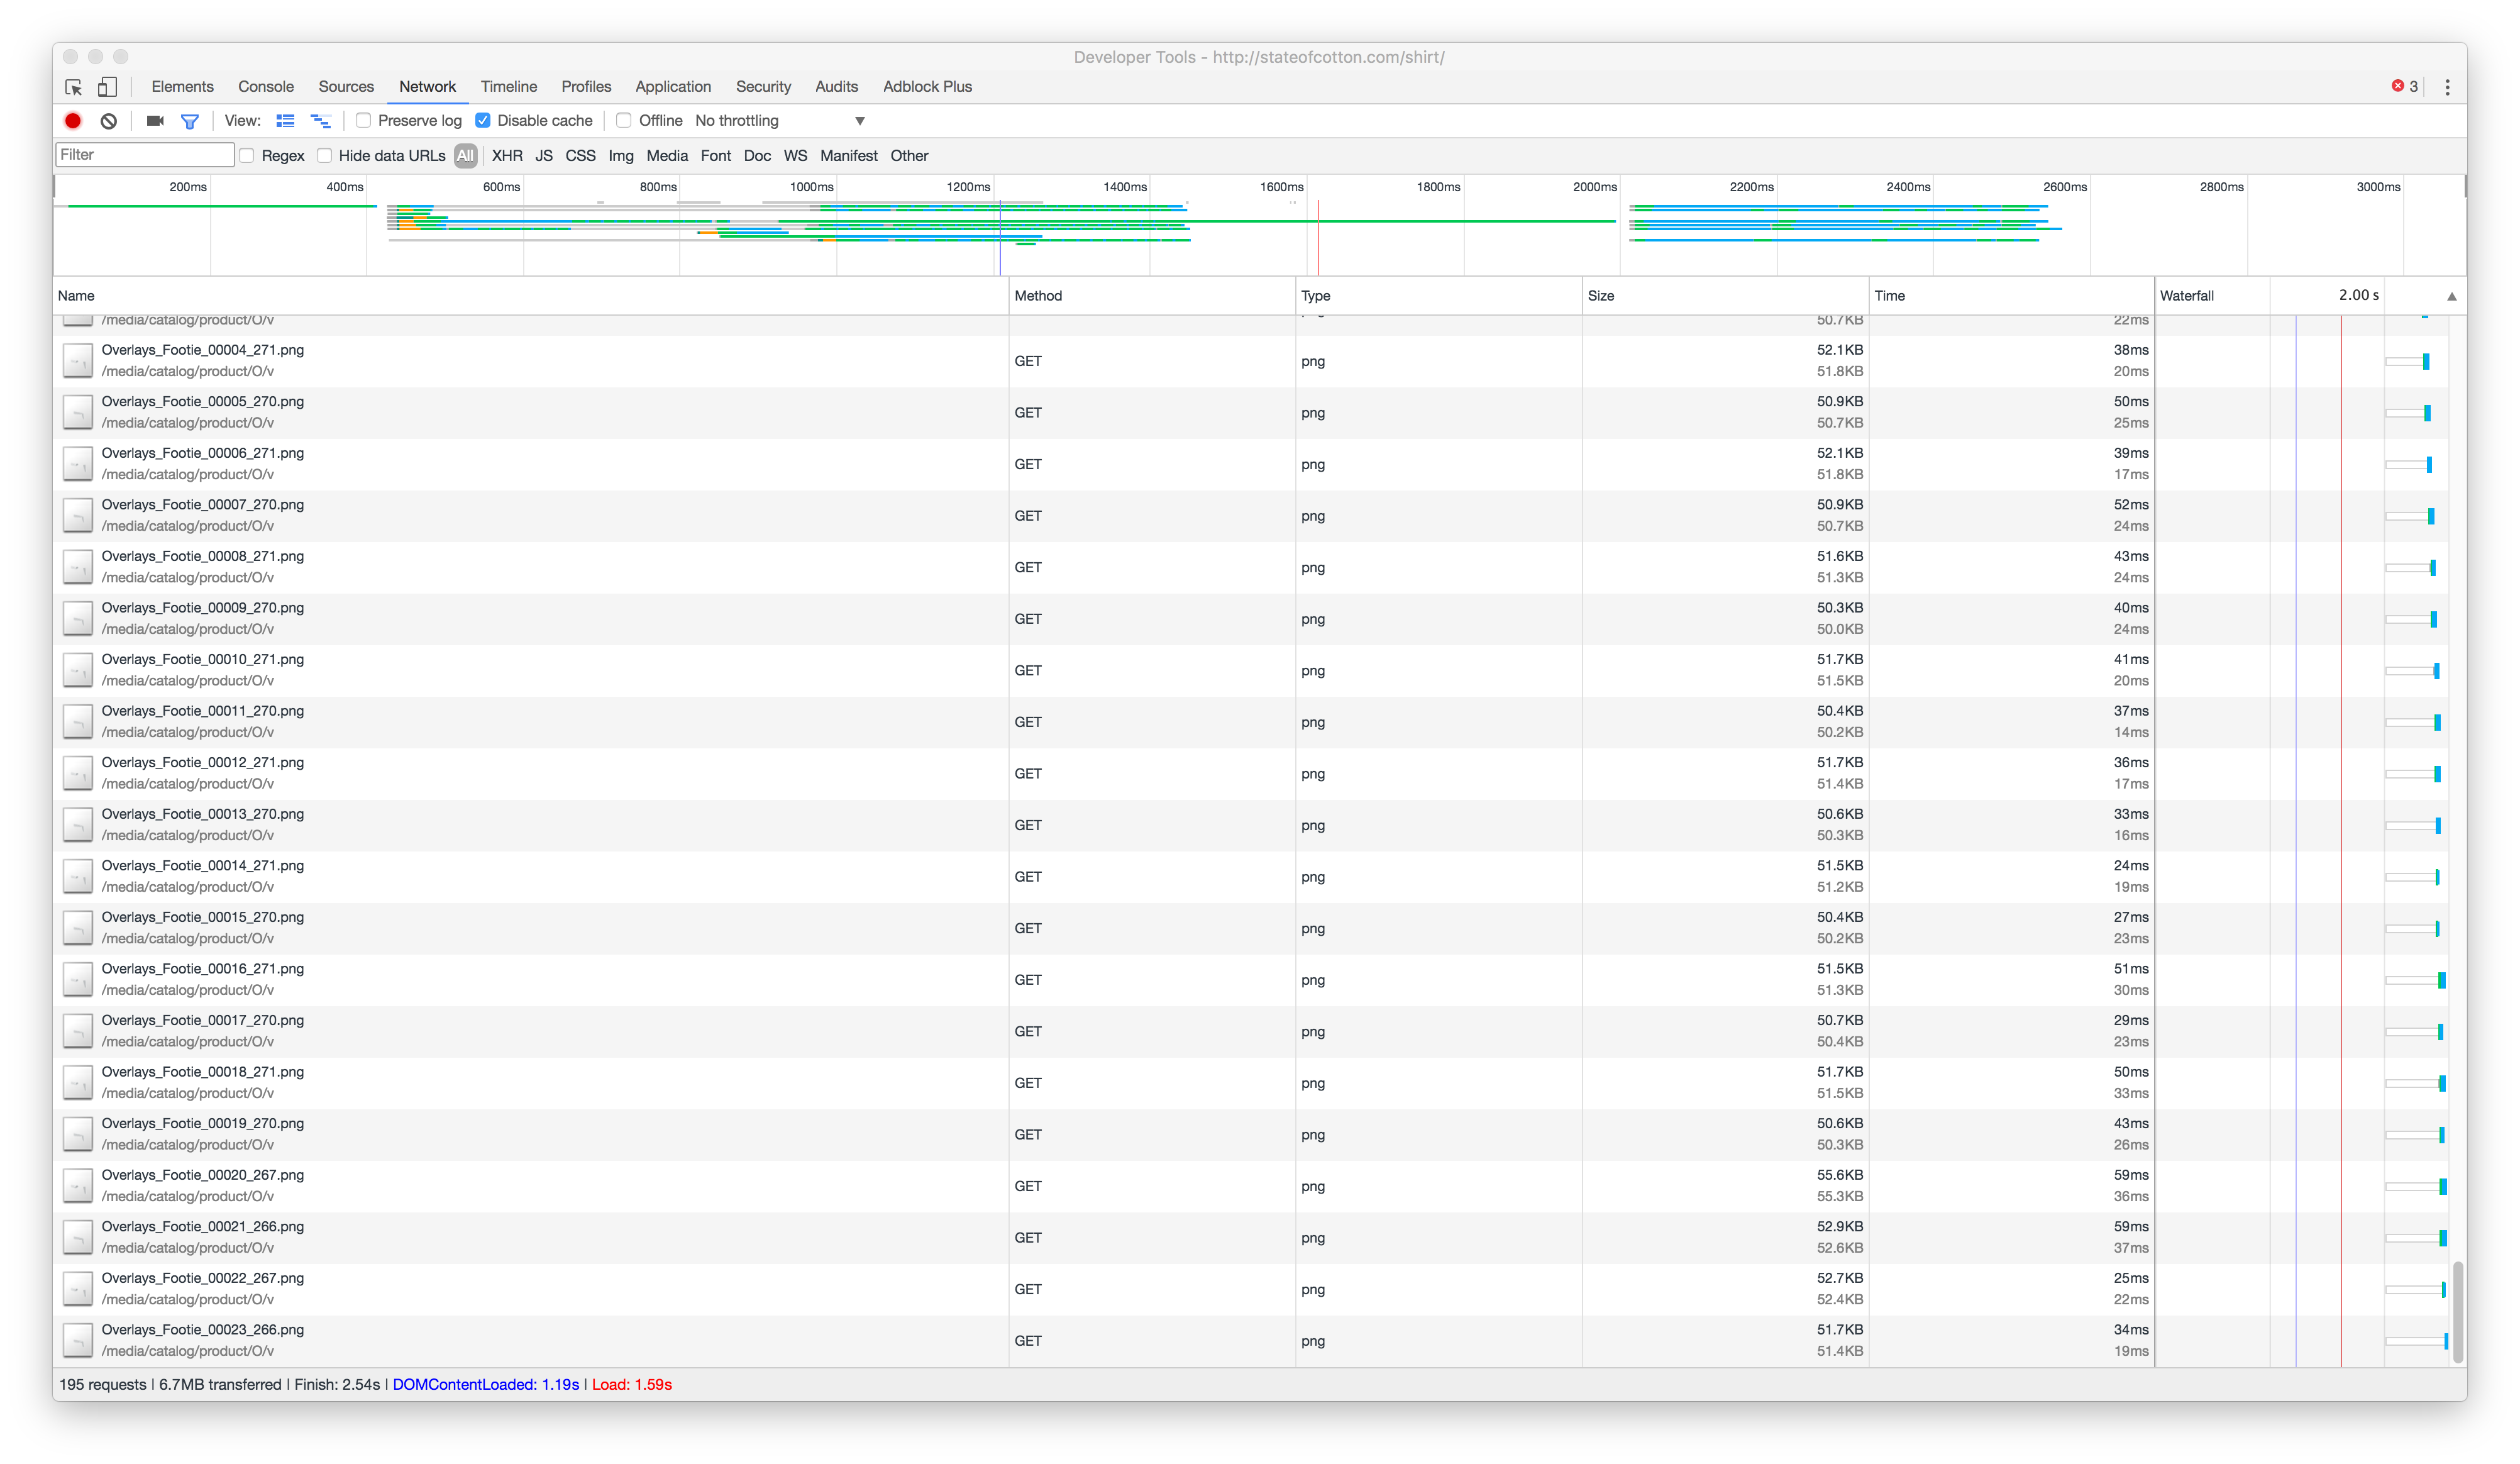
\includegraphics[width=15cm]{images/2componentsSwap}
\caption{Page Load 2 component swap SlimFitted}
\label{attachment:2componentsSwap}
\end{figure}

\begin{figure}
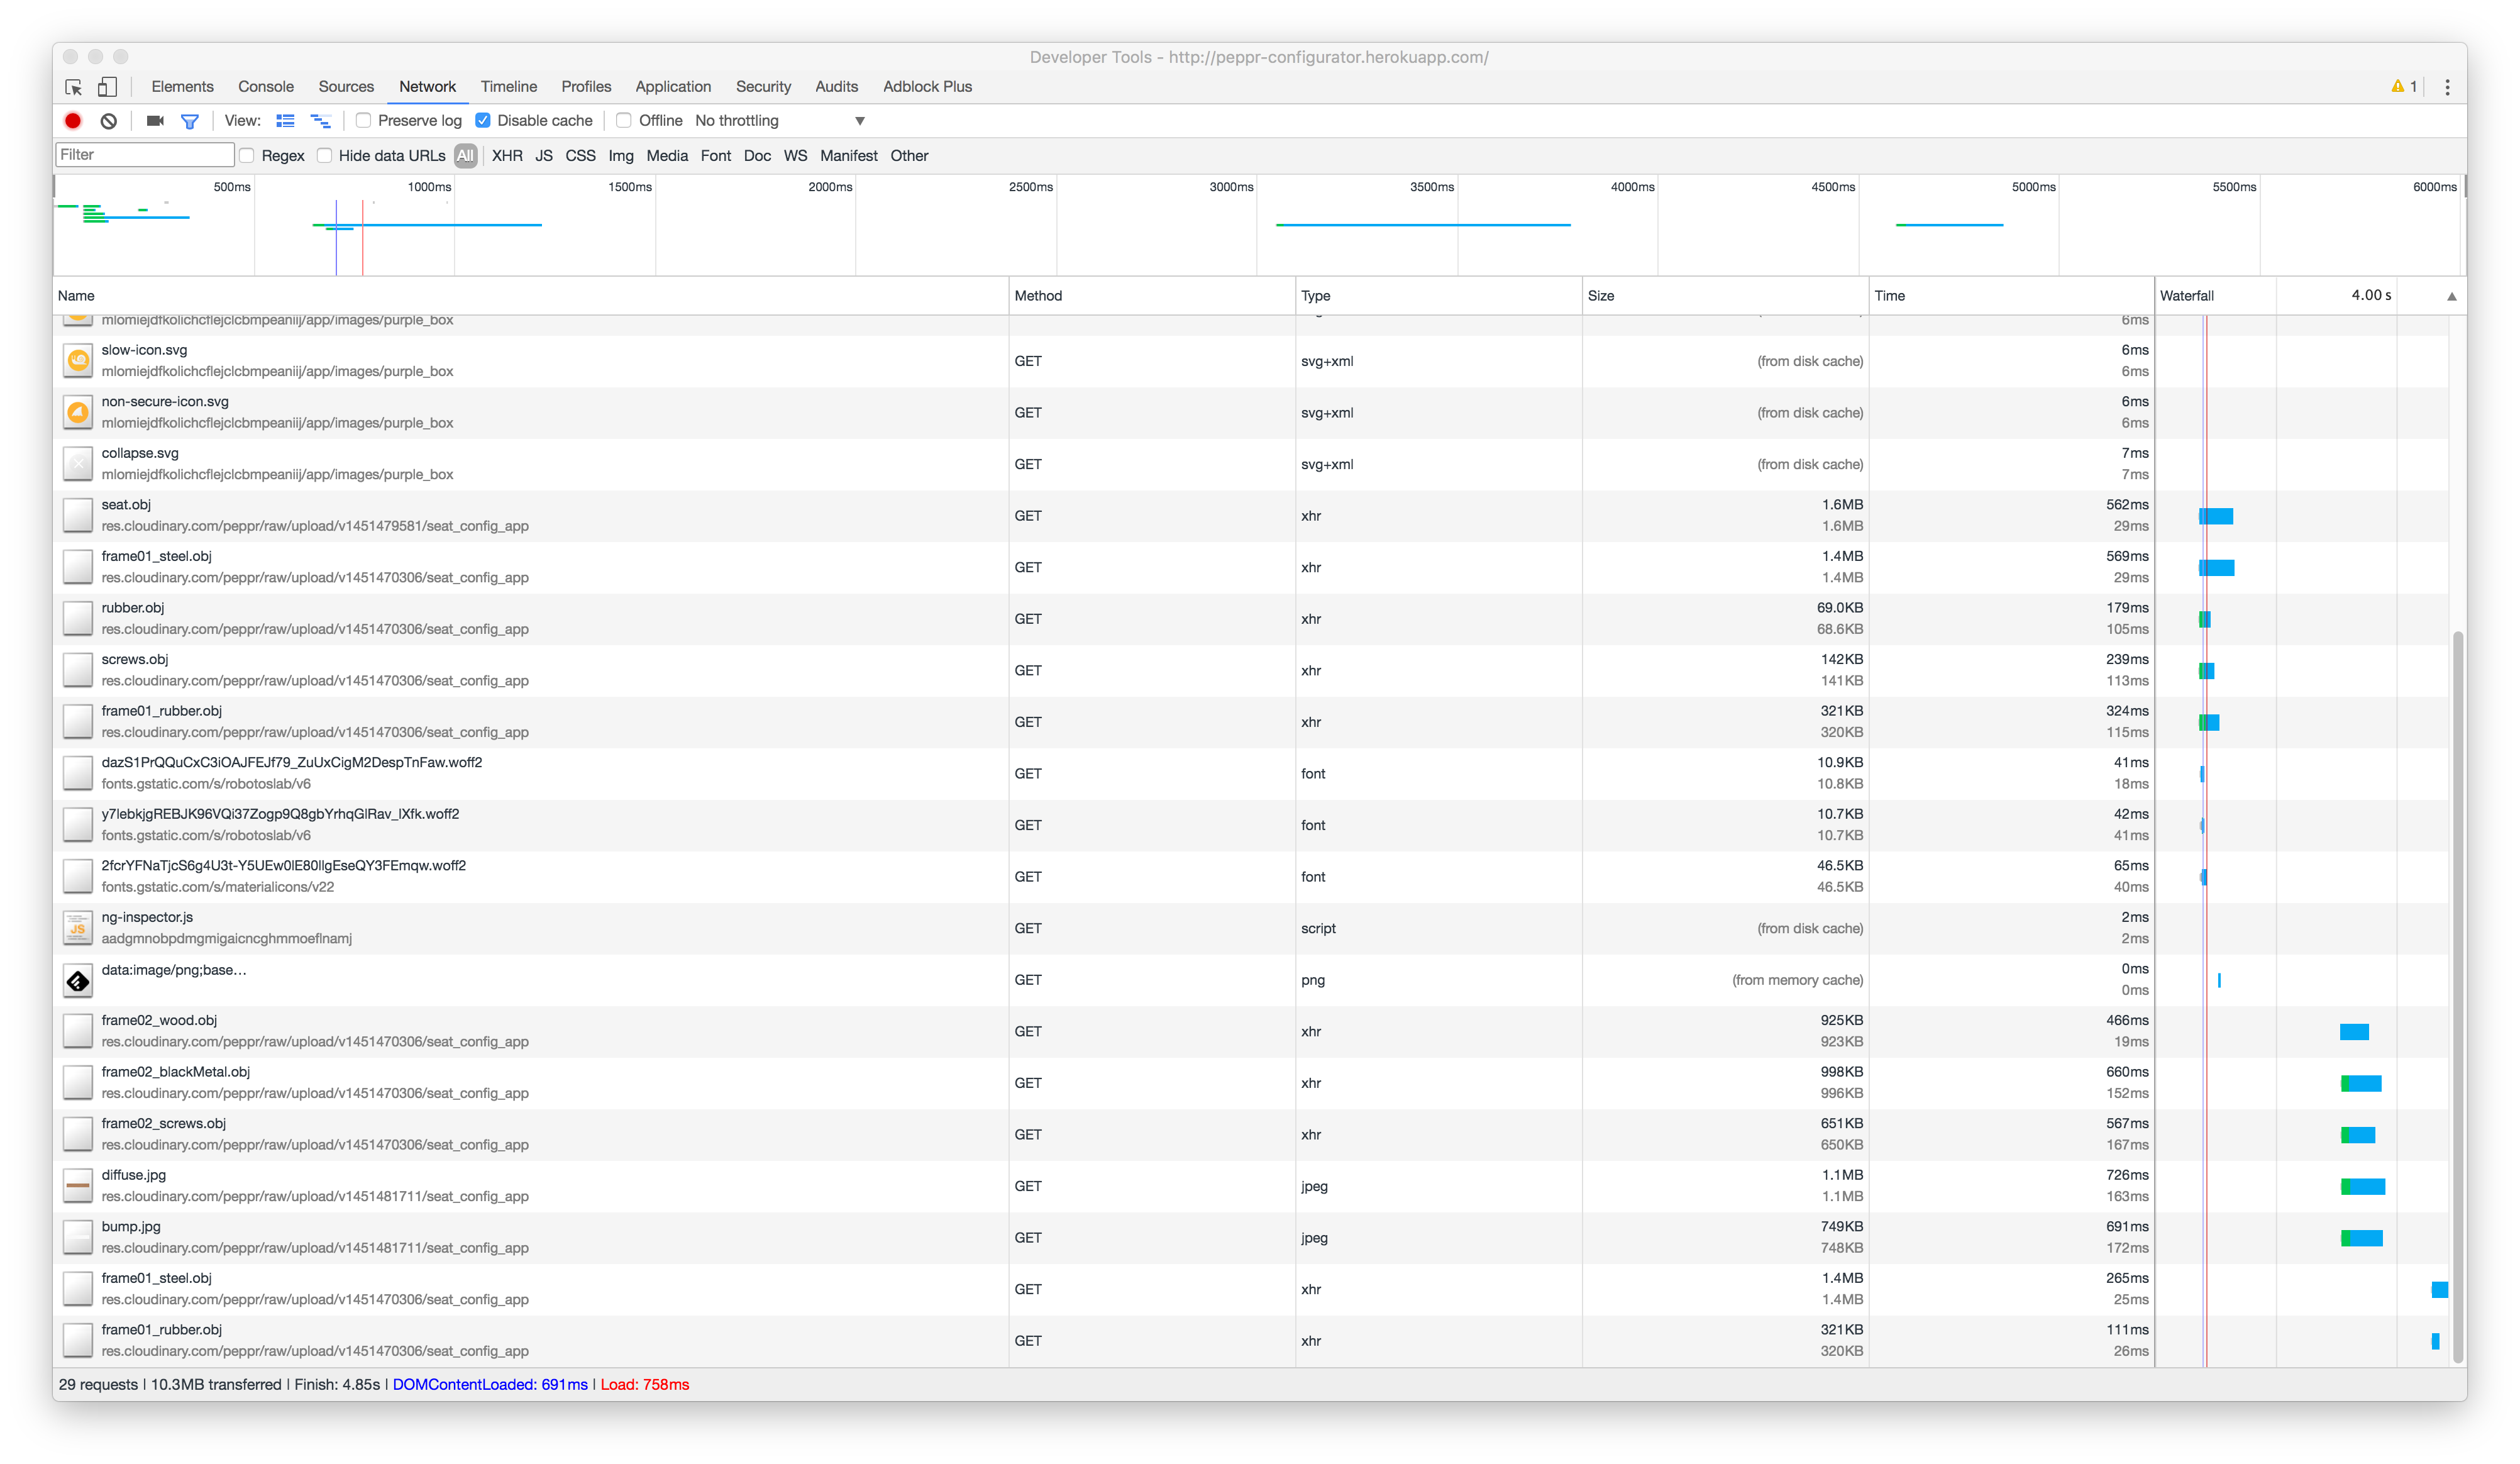
\includegraphics[width=15cm]{images/2componentsSwapWebGL}
\caption{Page Load 2 component swap WebGL}
\label{attachment:2componentsSwapWebGL}
\end{figure}

\clearpage

\begin{figure}
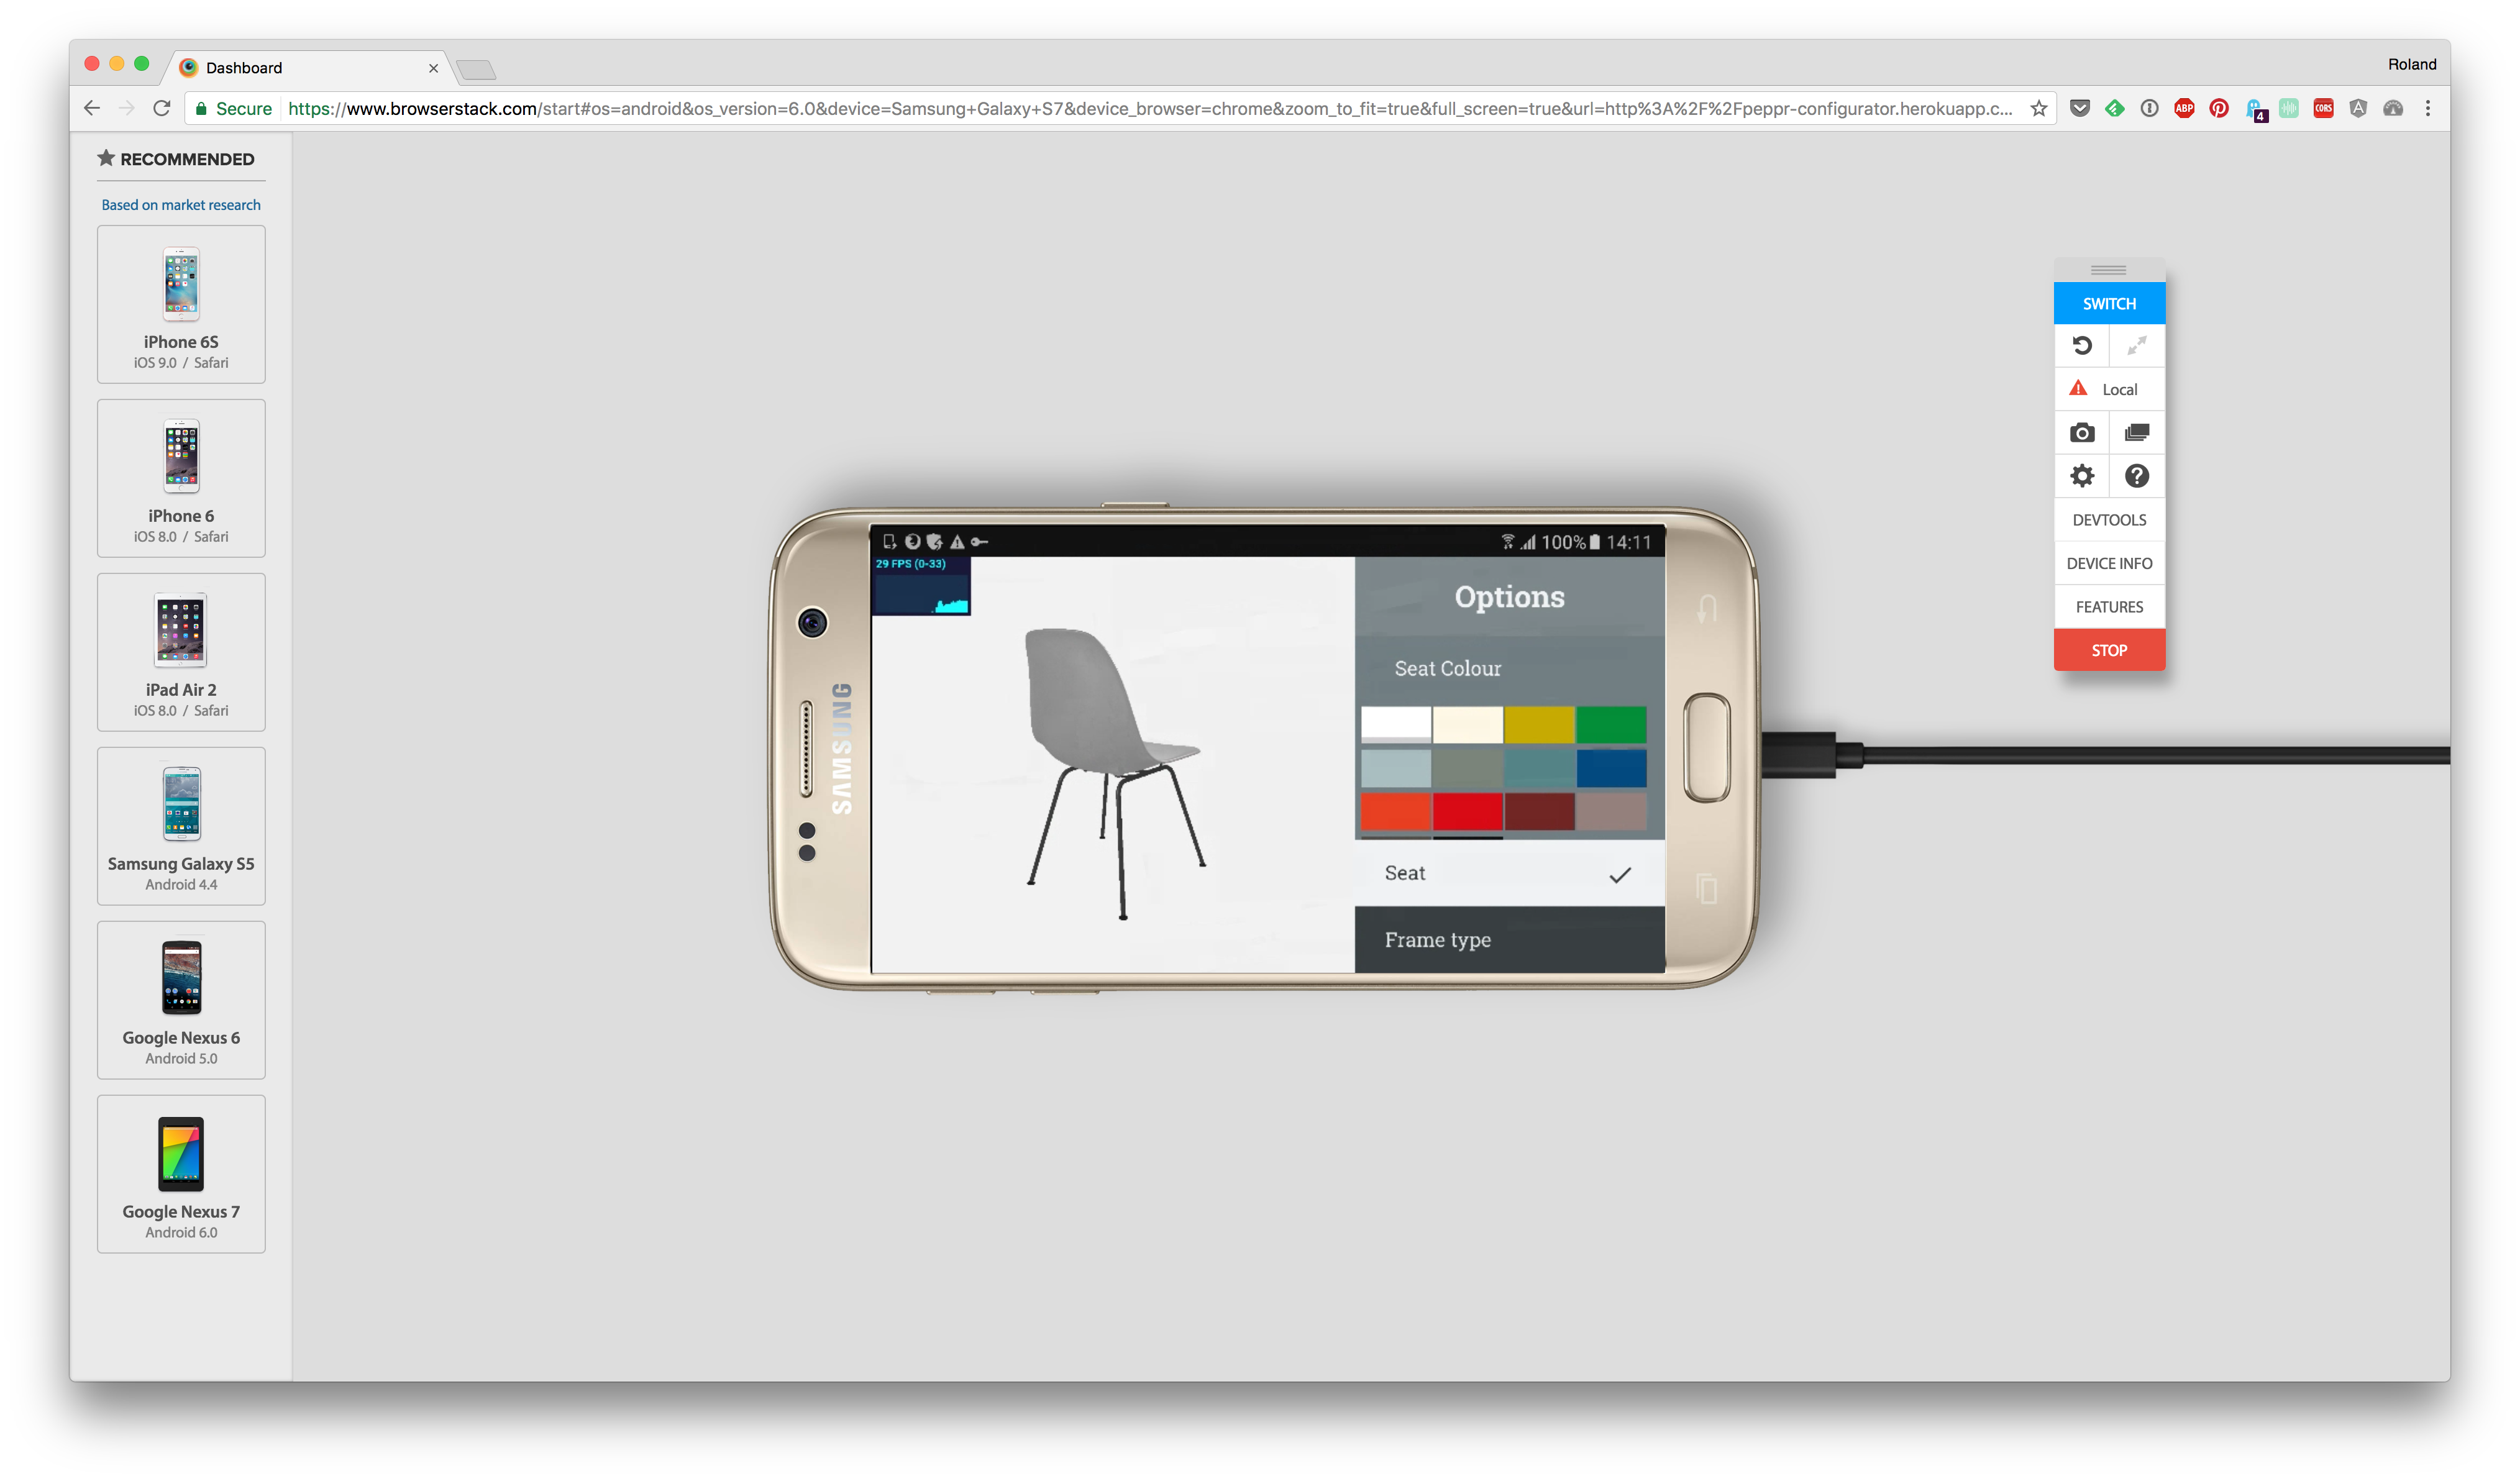
\includegraphics[width=15cm]{images/deviceScreenshots/GalaxyS7}
\caption{Browserstack screenshot: GalaxyS7}
\label{attachment:GalaxyS7}
\end{figure}

\begin{figure}

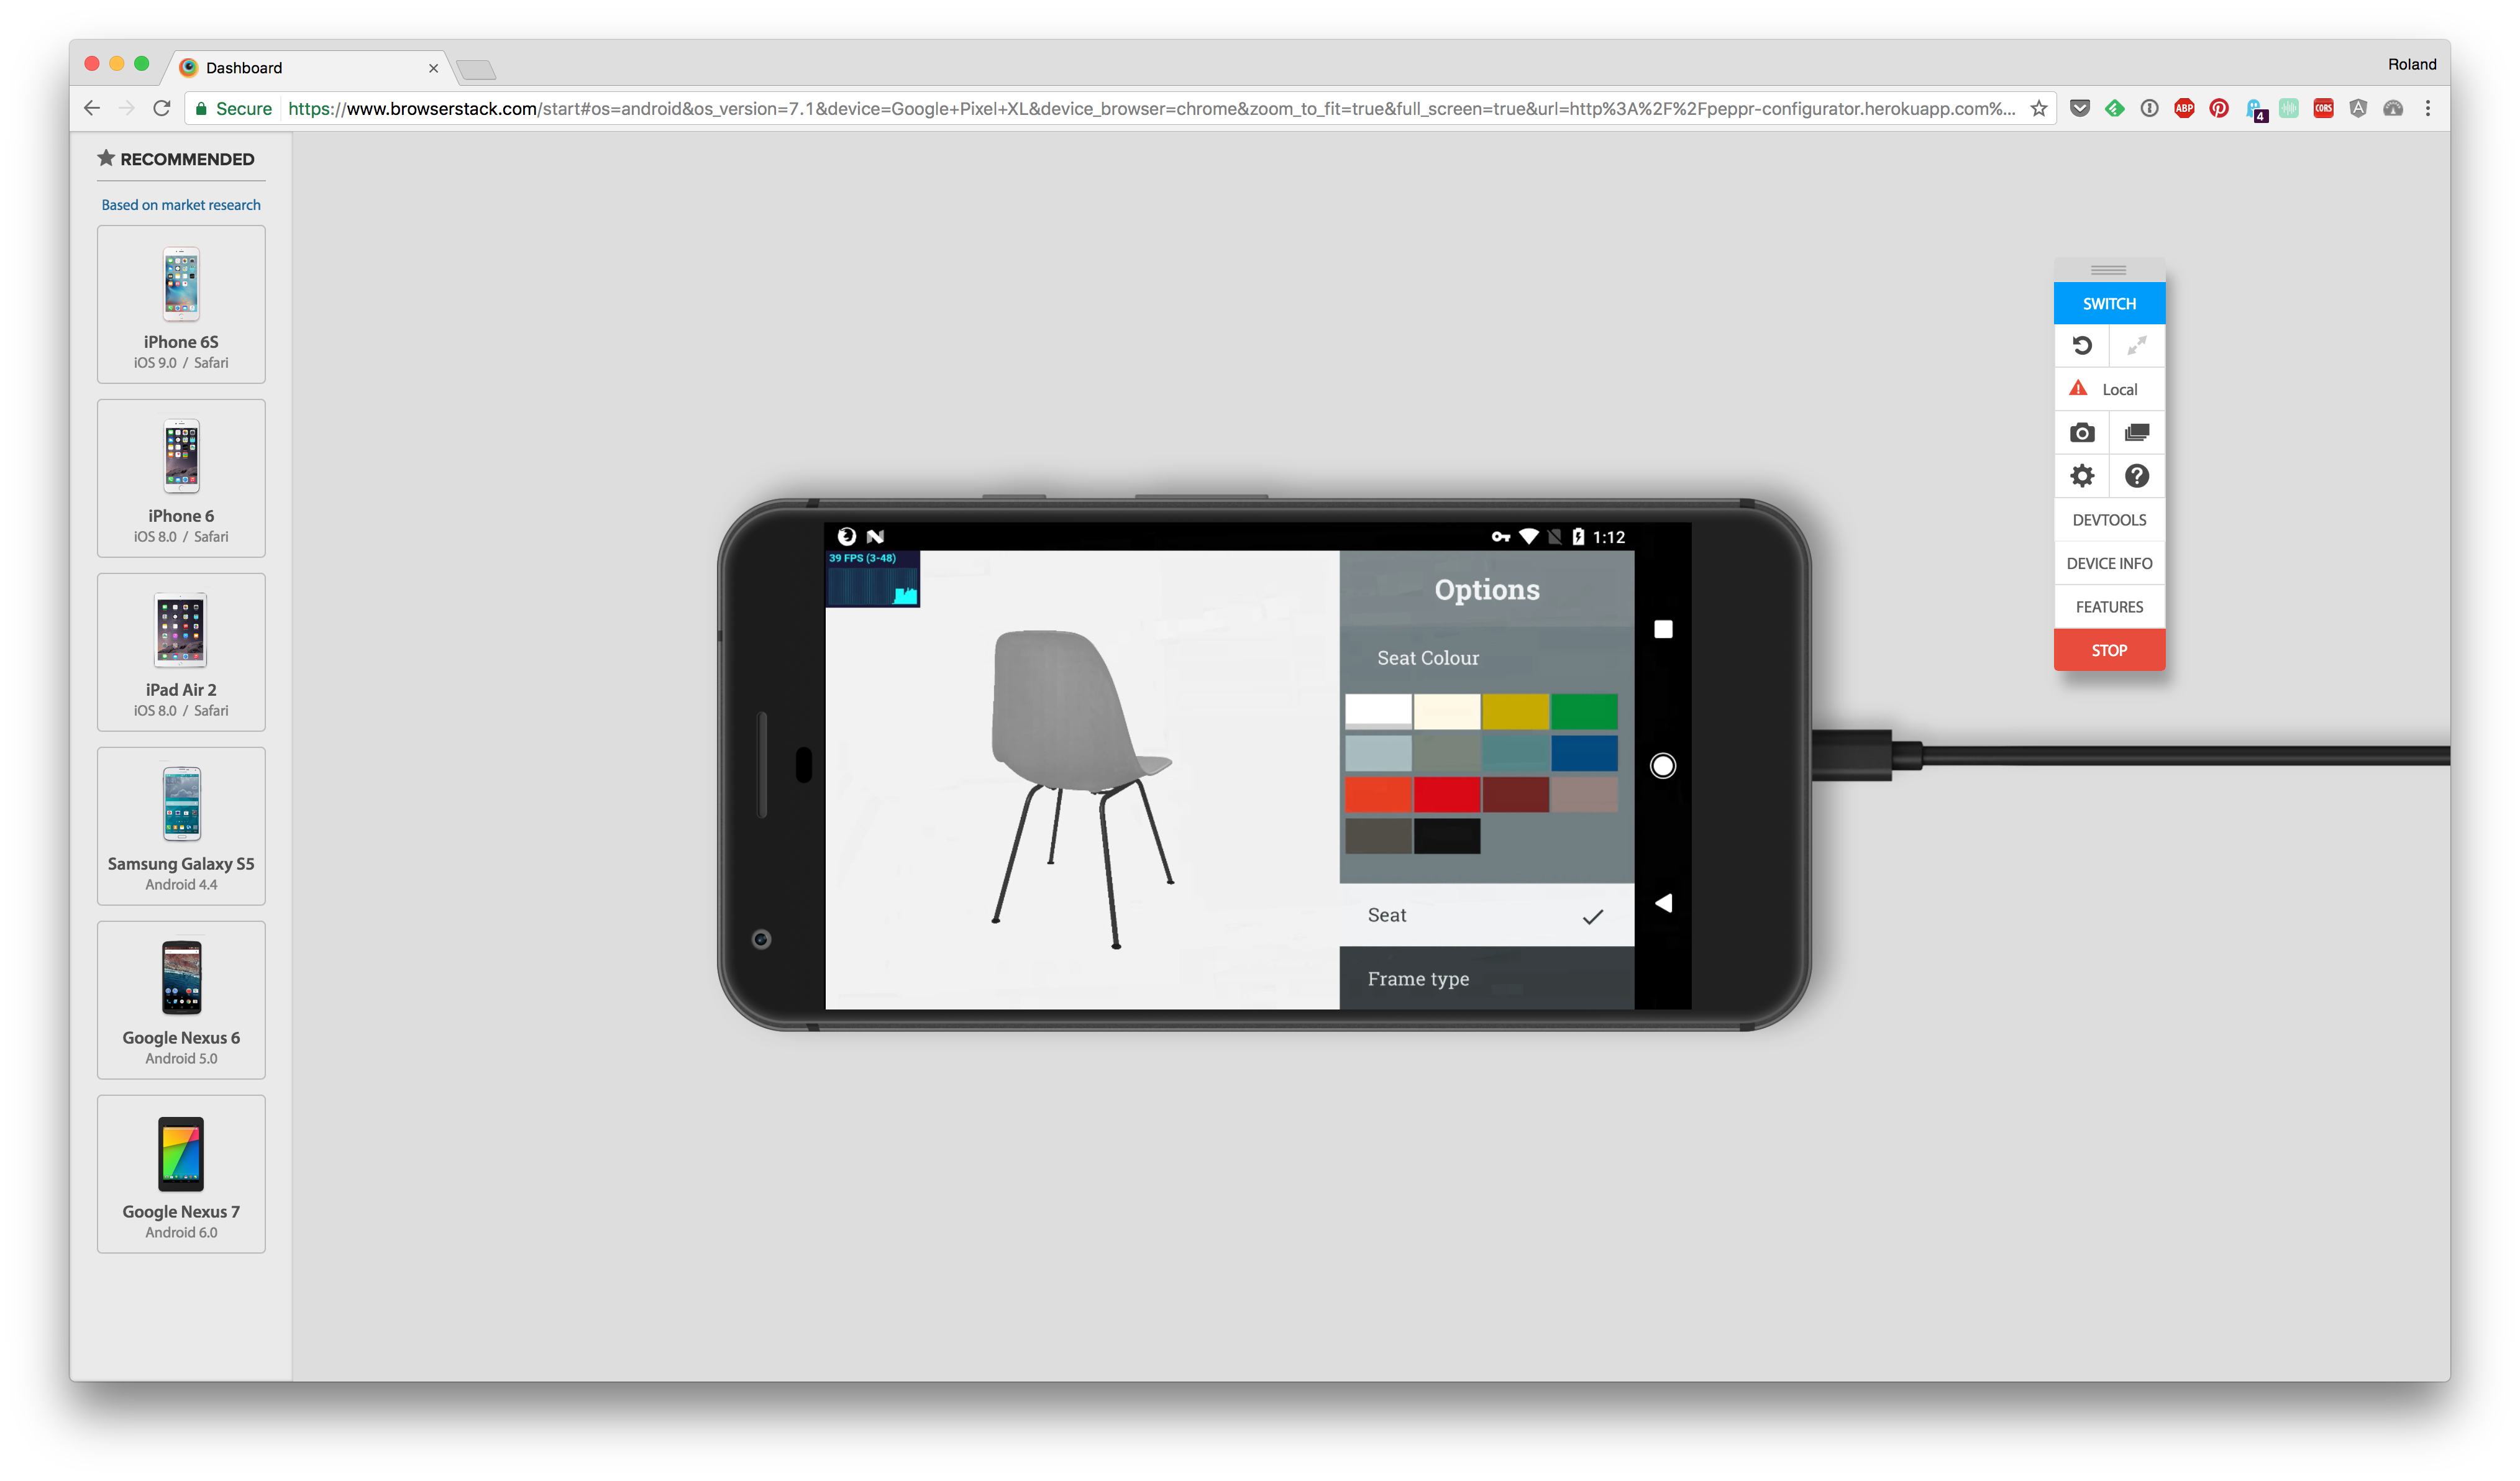
\includegraphics[width=15cm]{images/deviceScreenshots/GooglePixel}
\caption{Browserstack screenshot: GooglePixel}
\label{attachment:GooglePixel}
\end{figure}

\clearpage

\begin{figure}
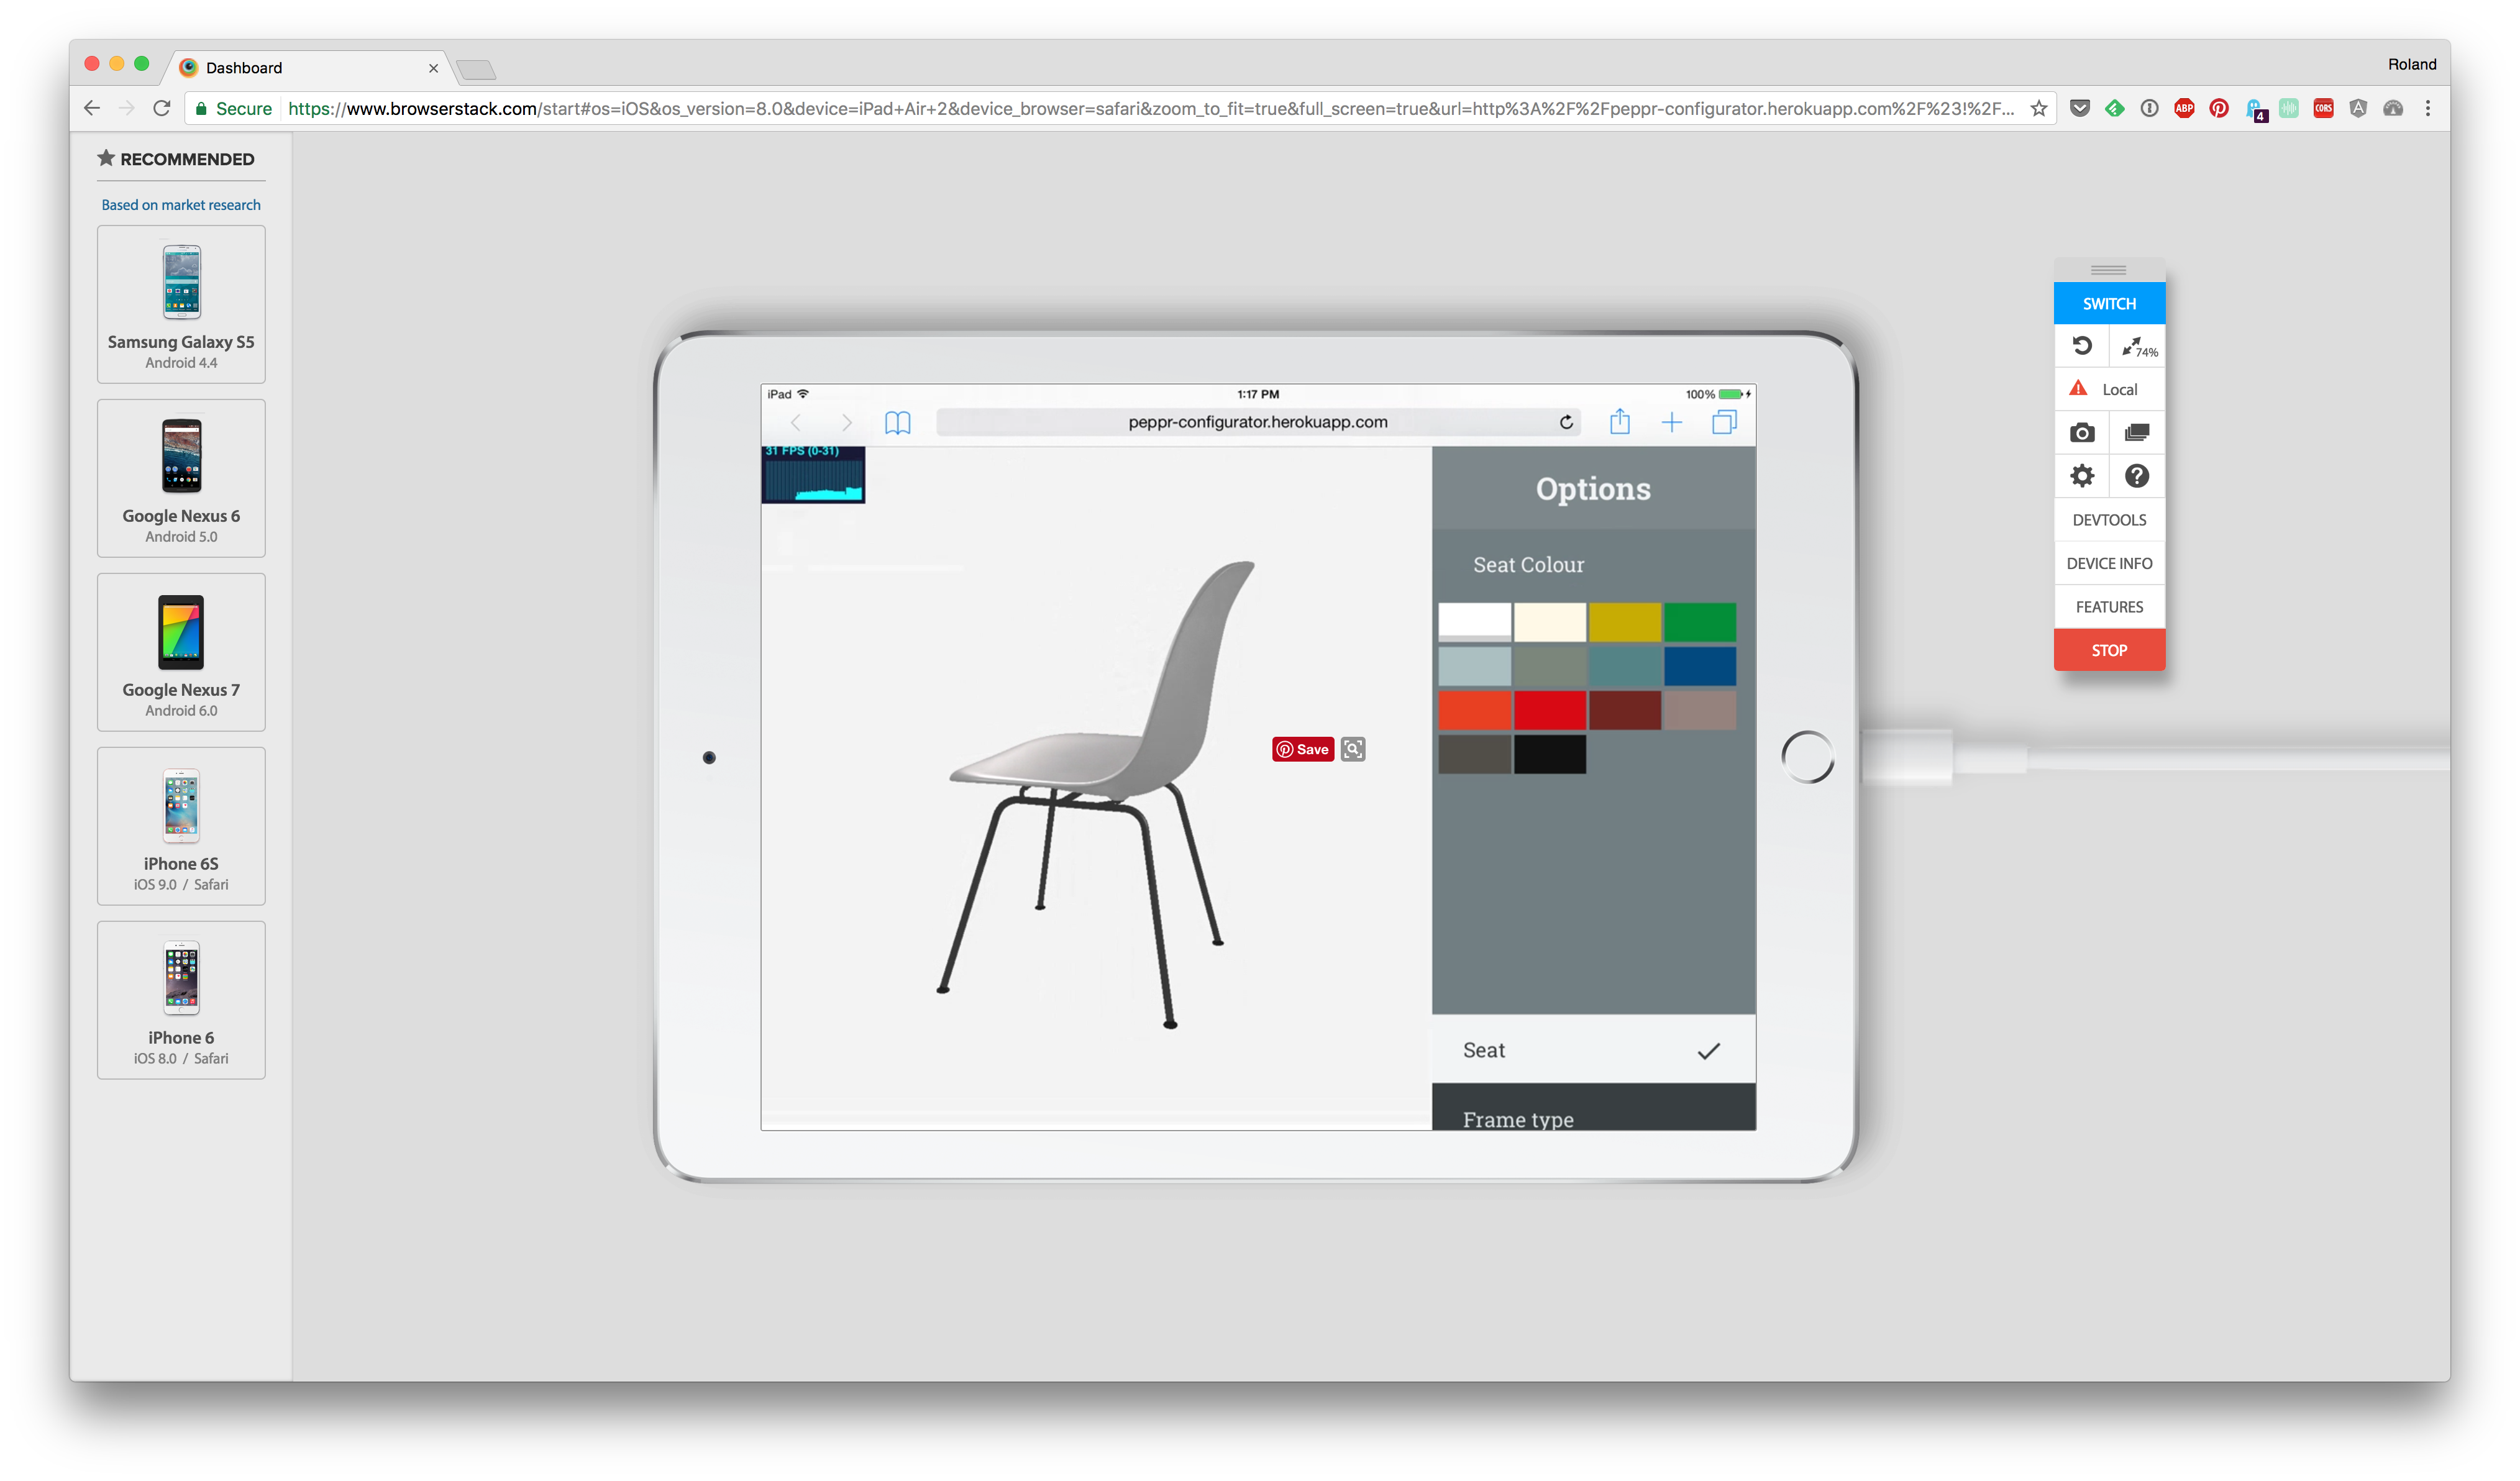
\includegraphics[width=15cm]{images/deviceScreenshots/iPadAir2}
\caption{Browserstack screenshot: iPadAir2}
\label{attachment:iPadAir2}
\end{figure}

\begin{figure}
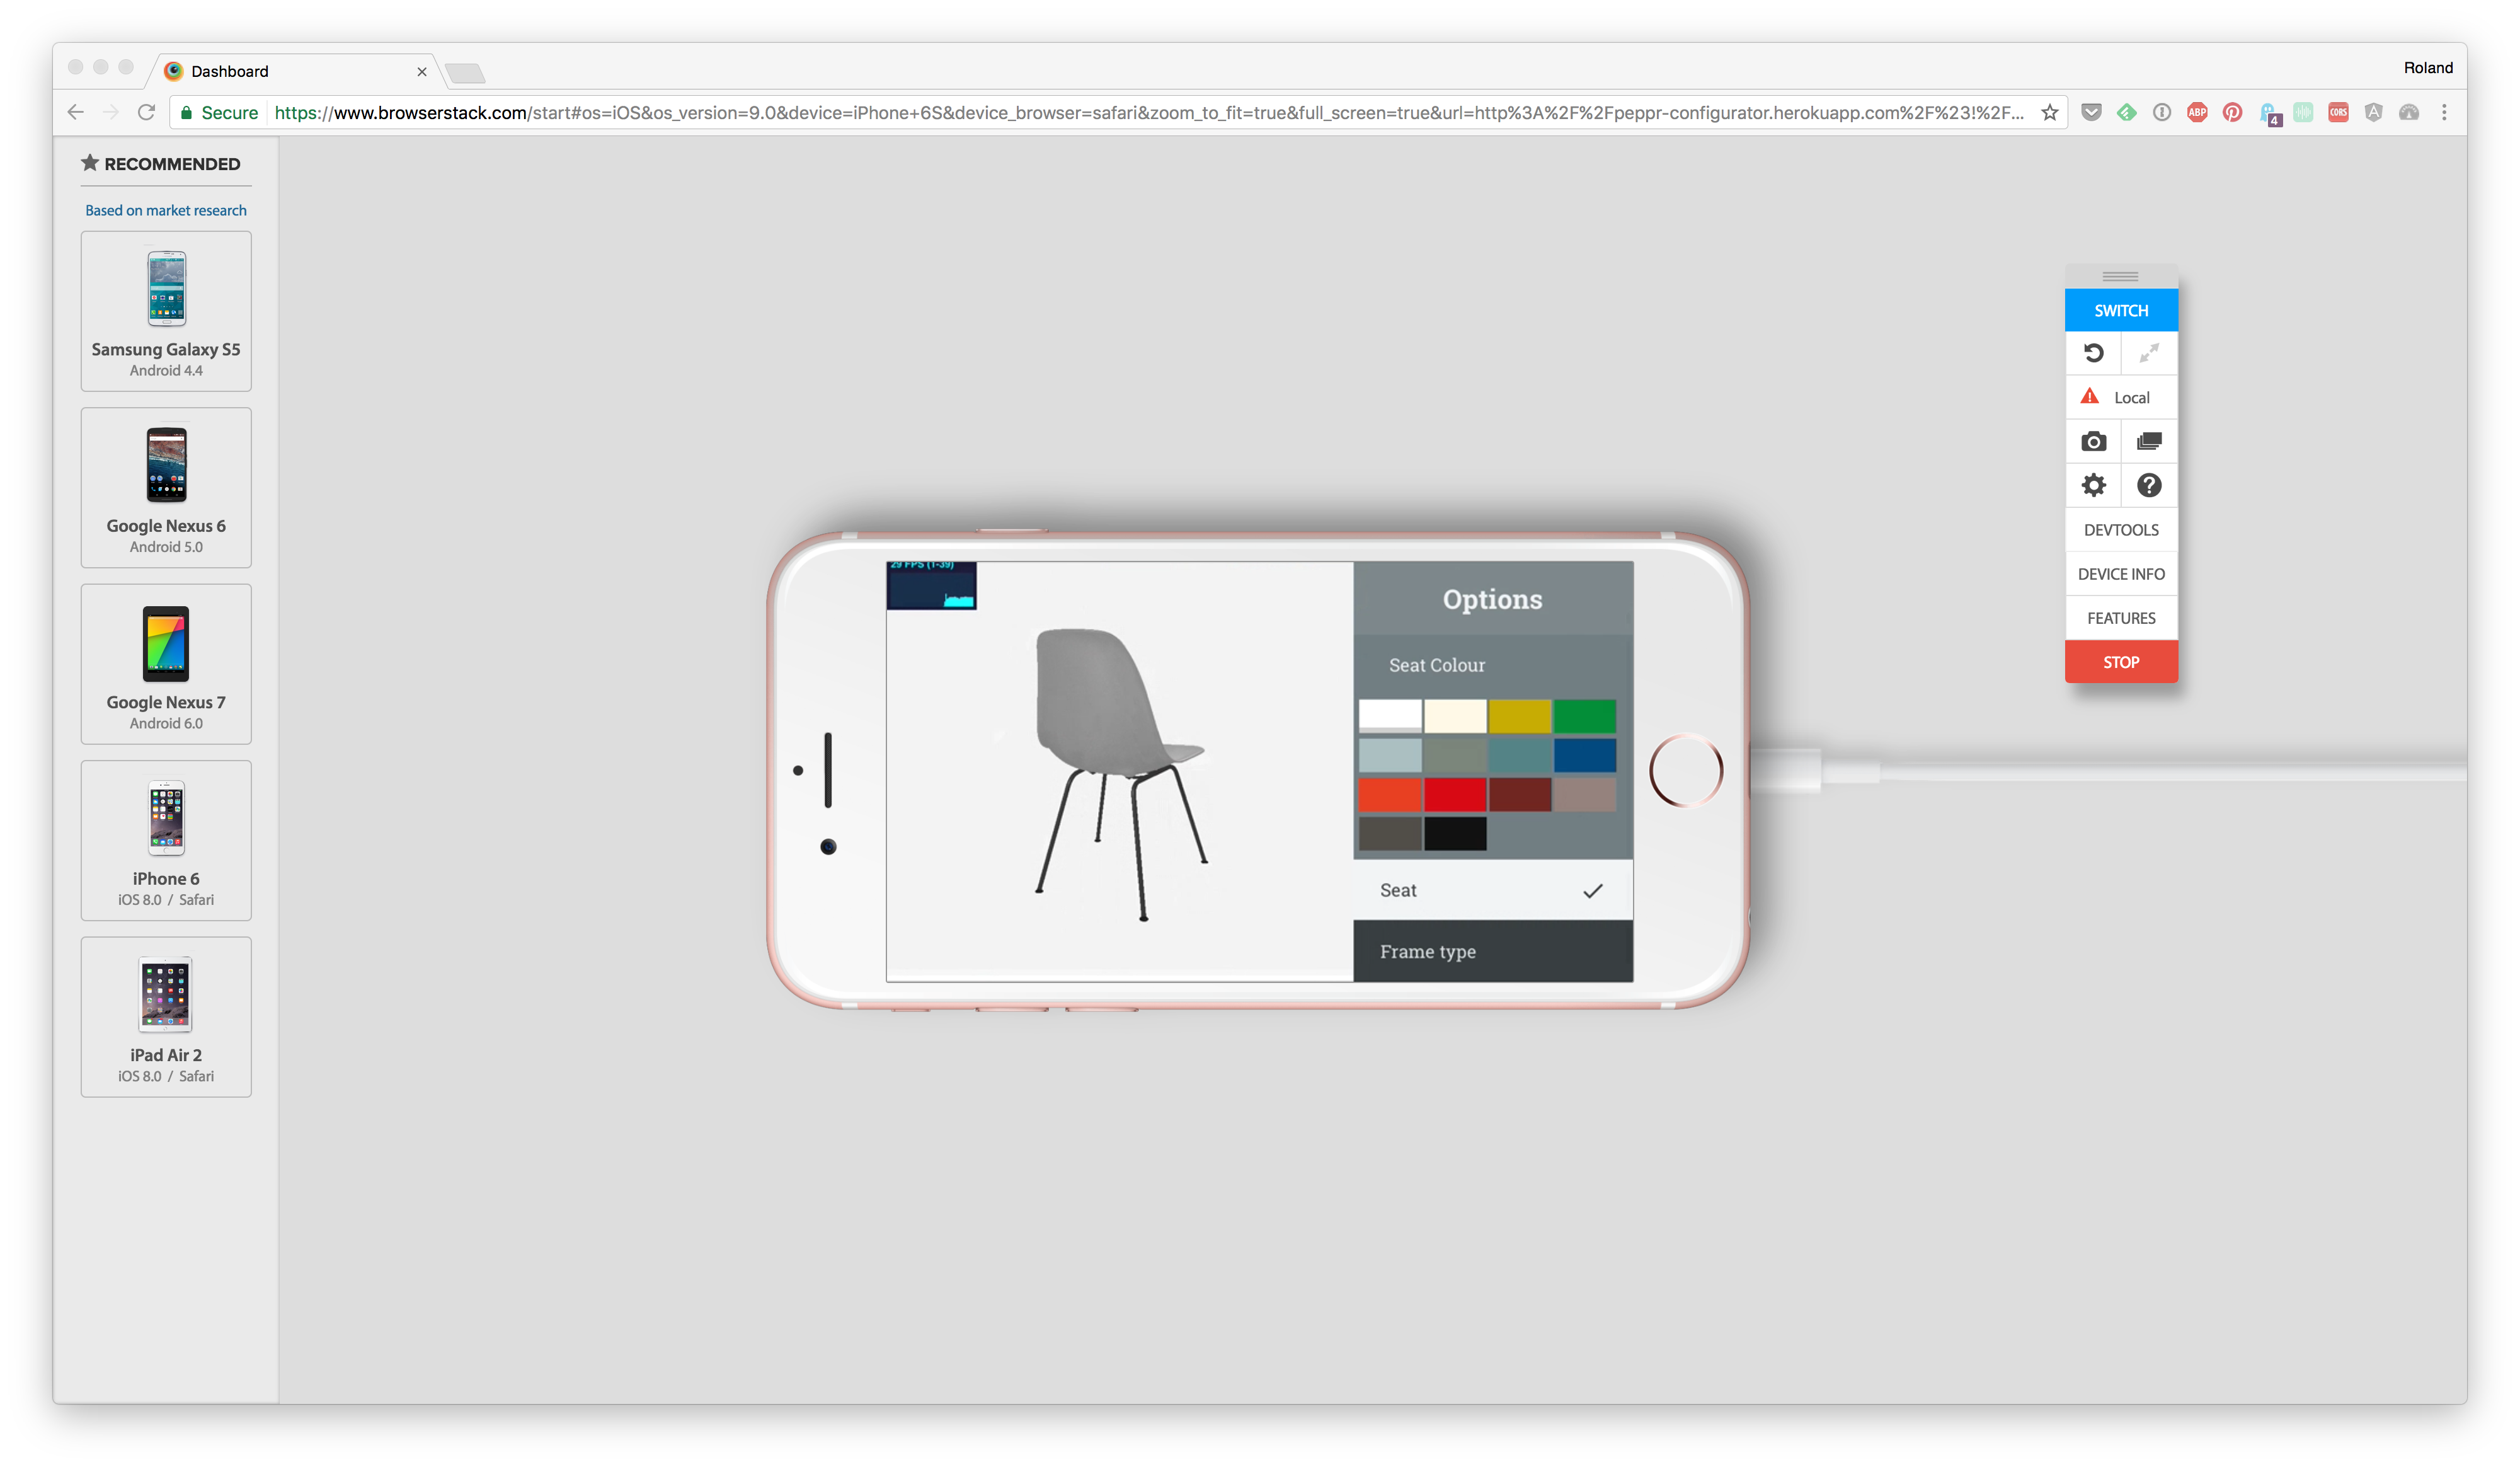
\includegraphics[width=15cm]{images/deviceScreenshots/iPhone6s}
\caption{Browserstack screenshot: iPhone6s}
\label{attachment:iPhone6s}
\end{figure}

\clearpage

\begin{figure}
\includegraphics[width=15cm]{images/deviceScreenshots/iPhone7}
\caption{Browserstack screenshot: iPhone7}
\label{attachment:iPhone7}
\end{figure}

\begin{figure}
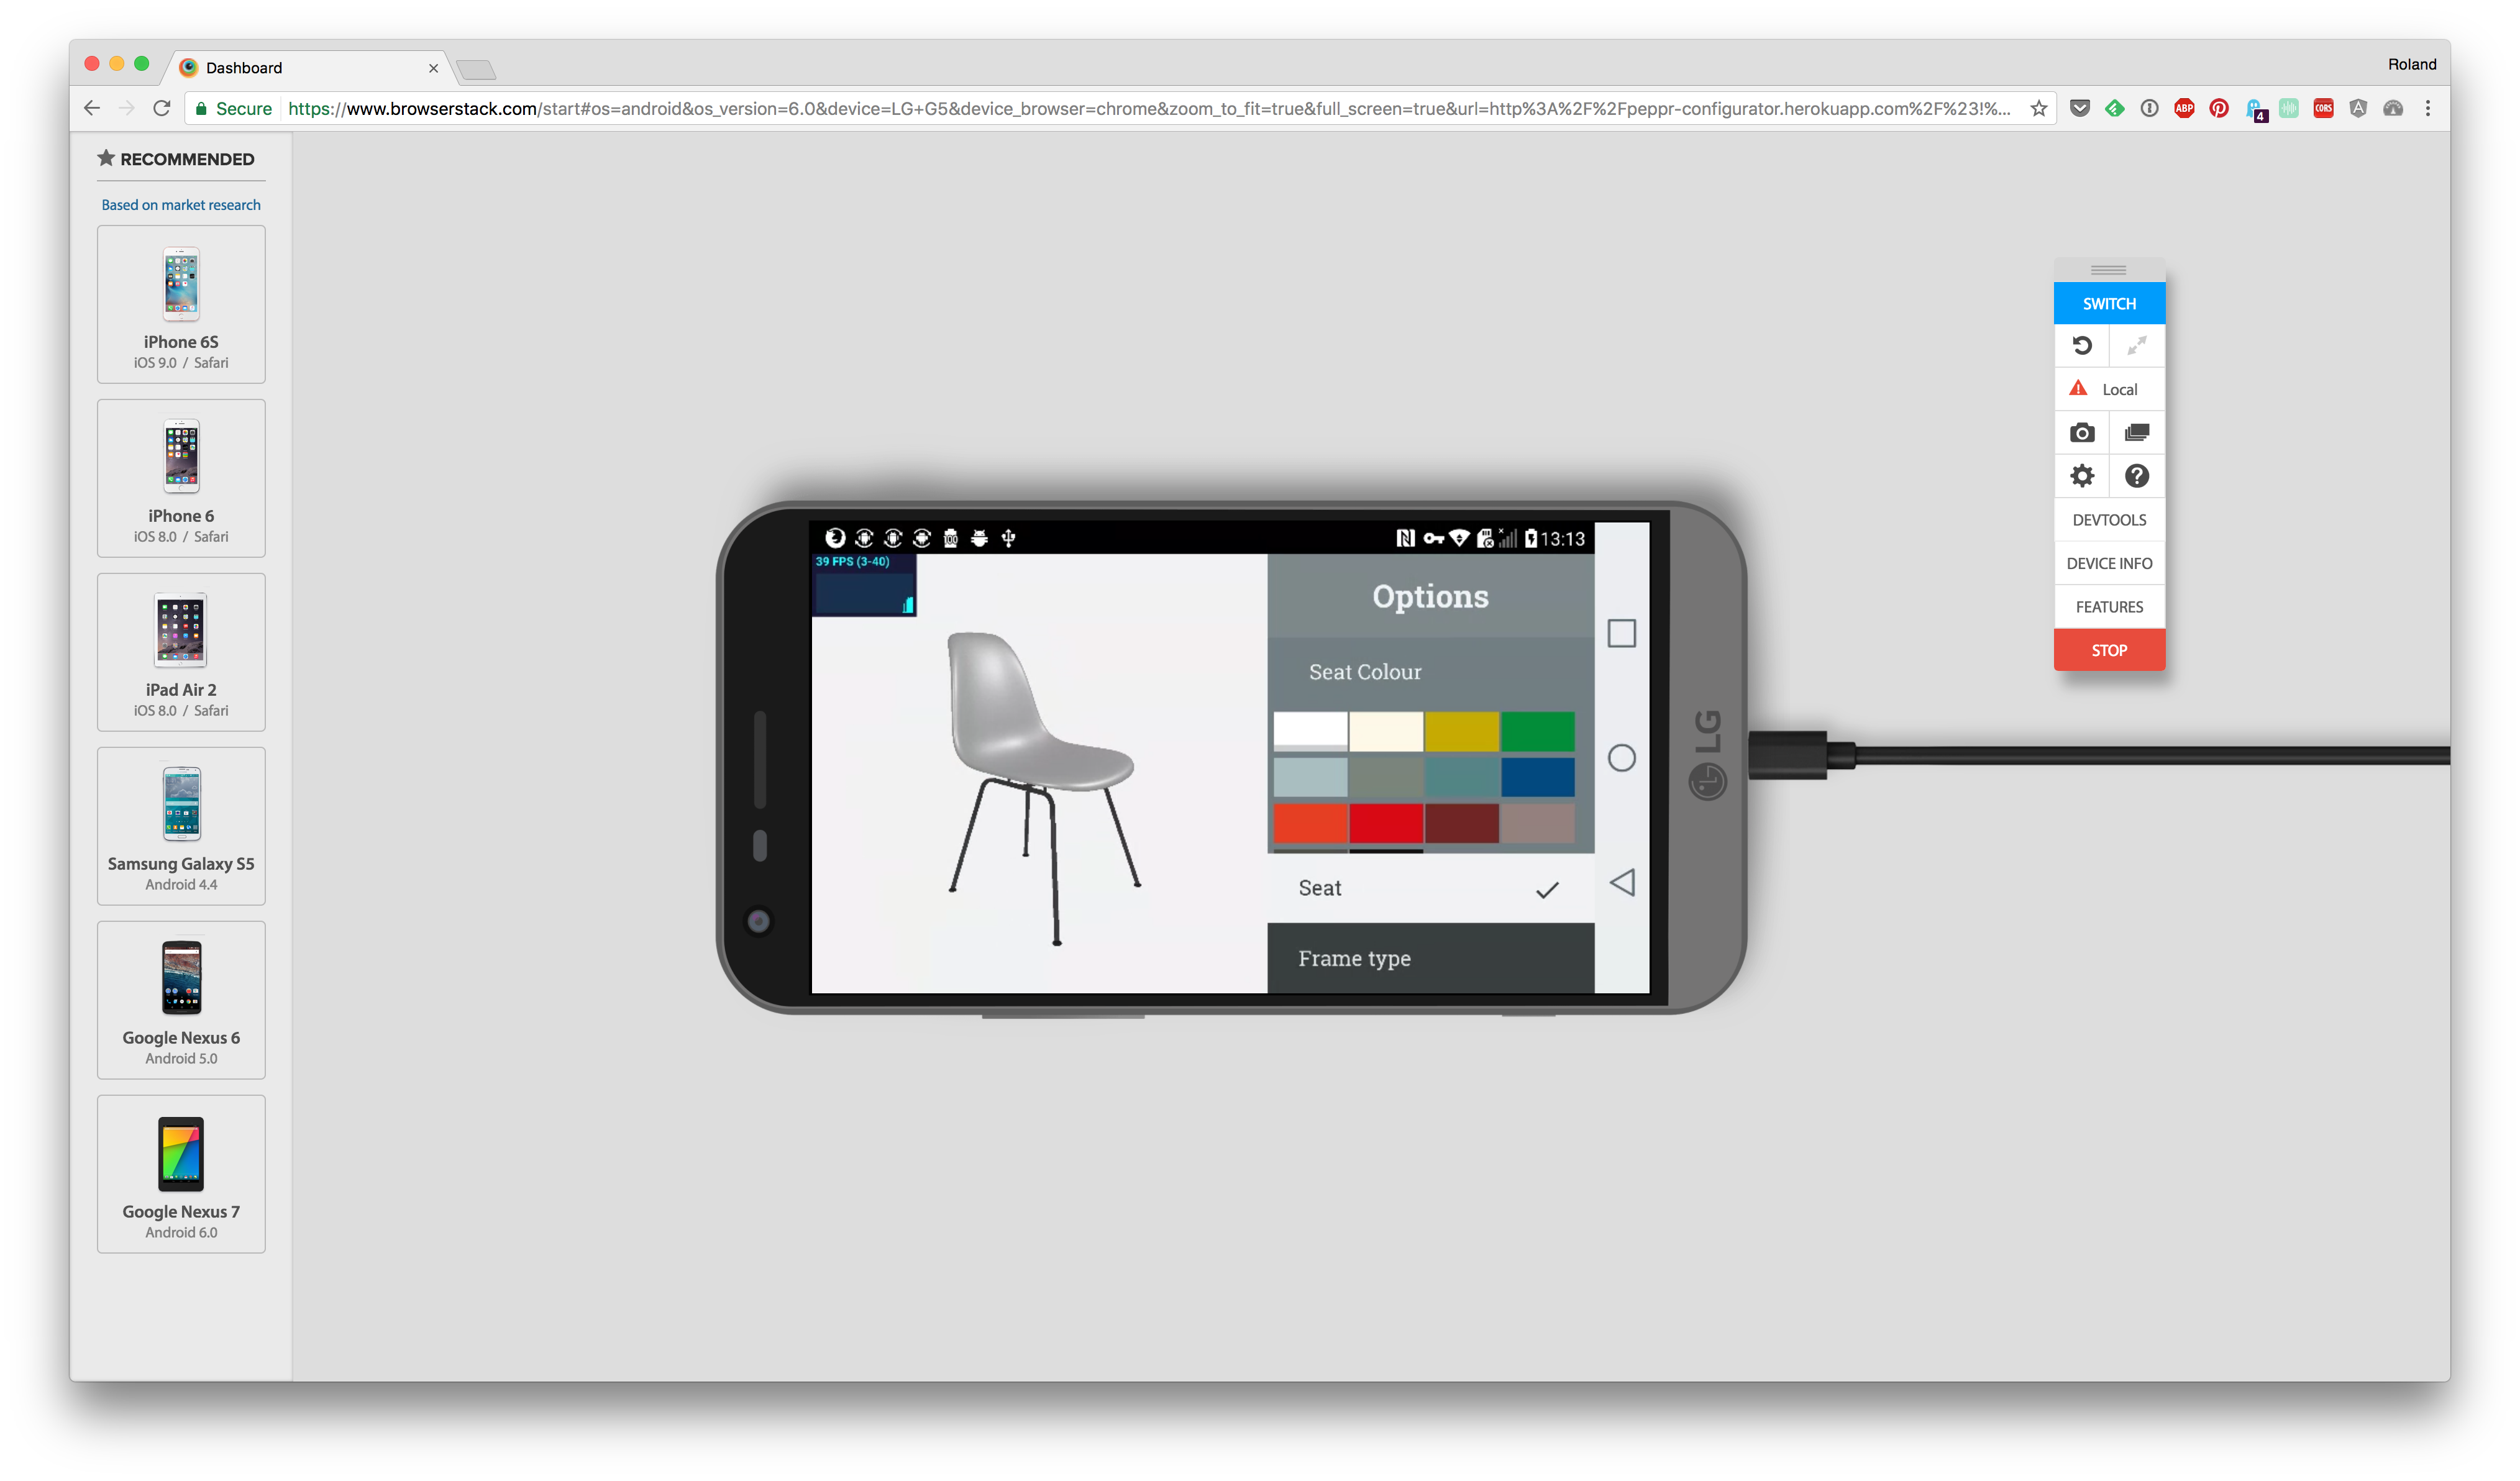
\includegraphics[width=15cm]{images/deviceScreenshots/LGG5}
\caption{Browserstack screenshot: LGG5}
\label{attachment:LGG5}
\end{figure}

\clearpage

\begin{figure}
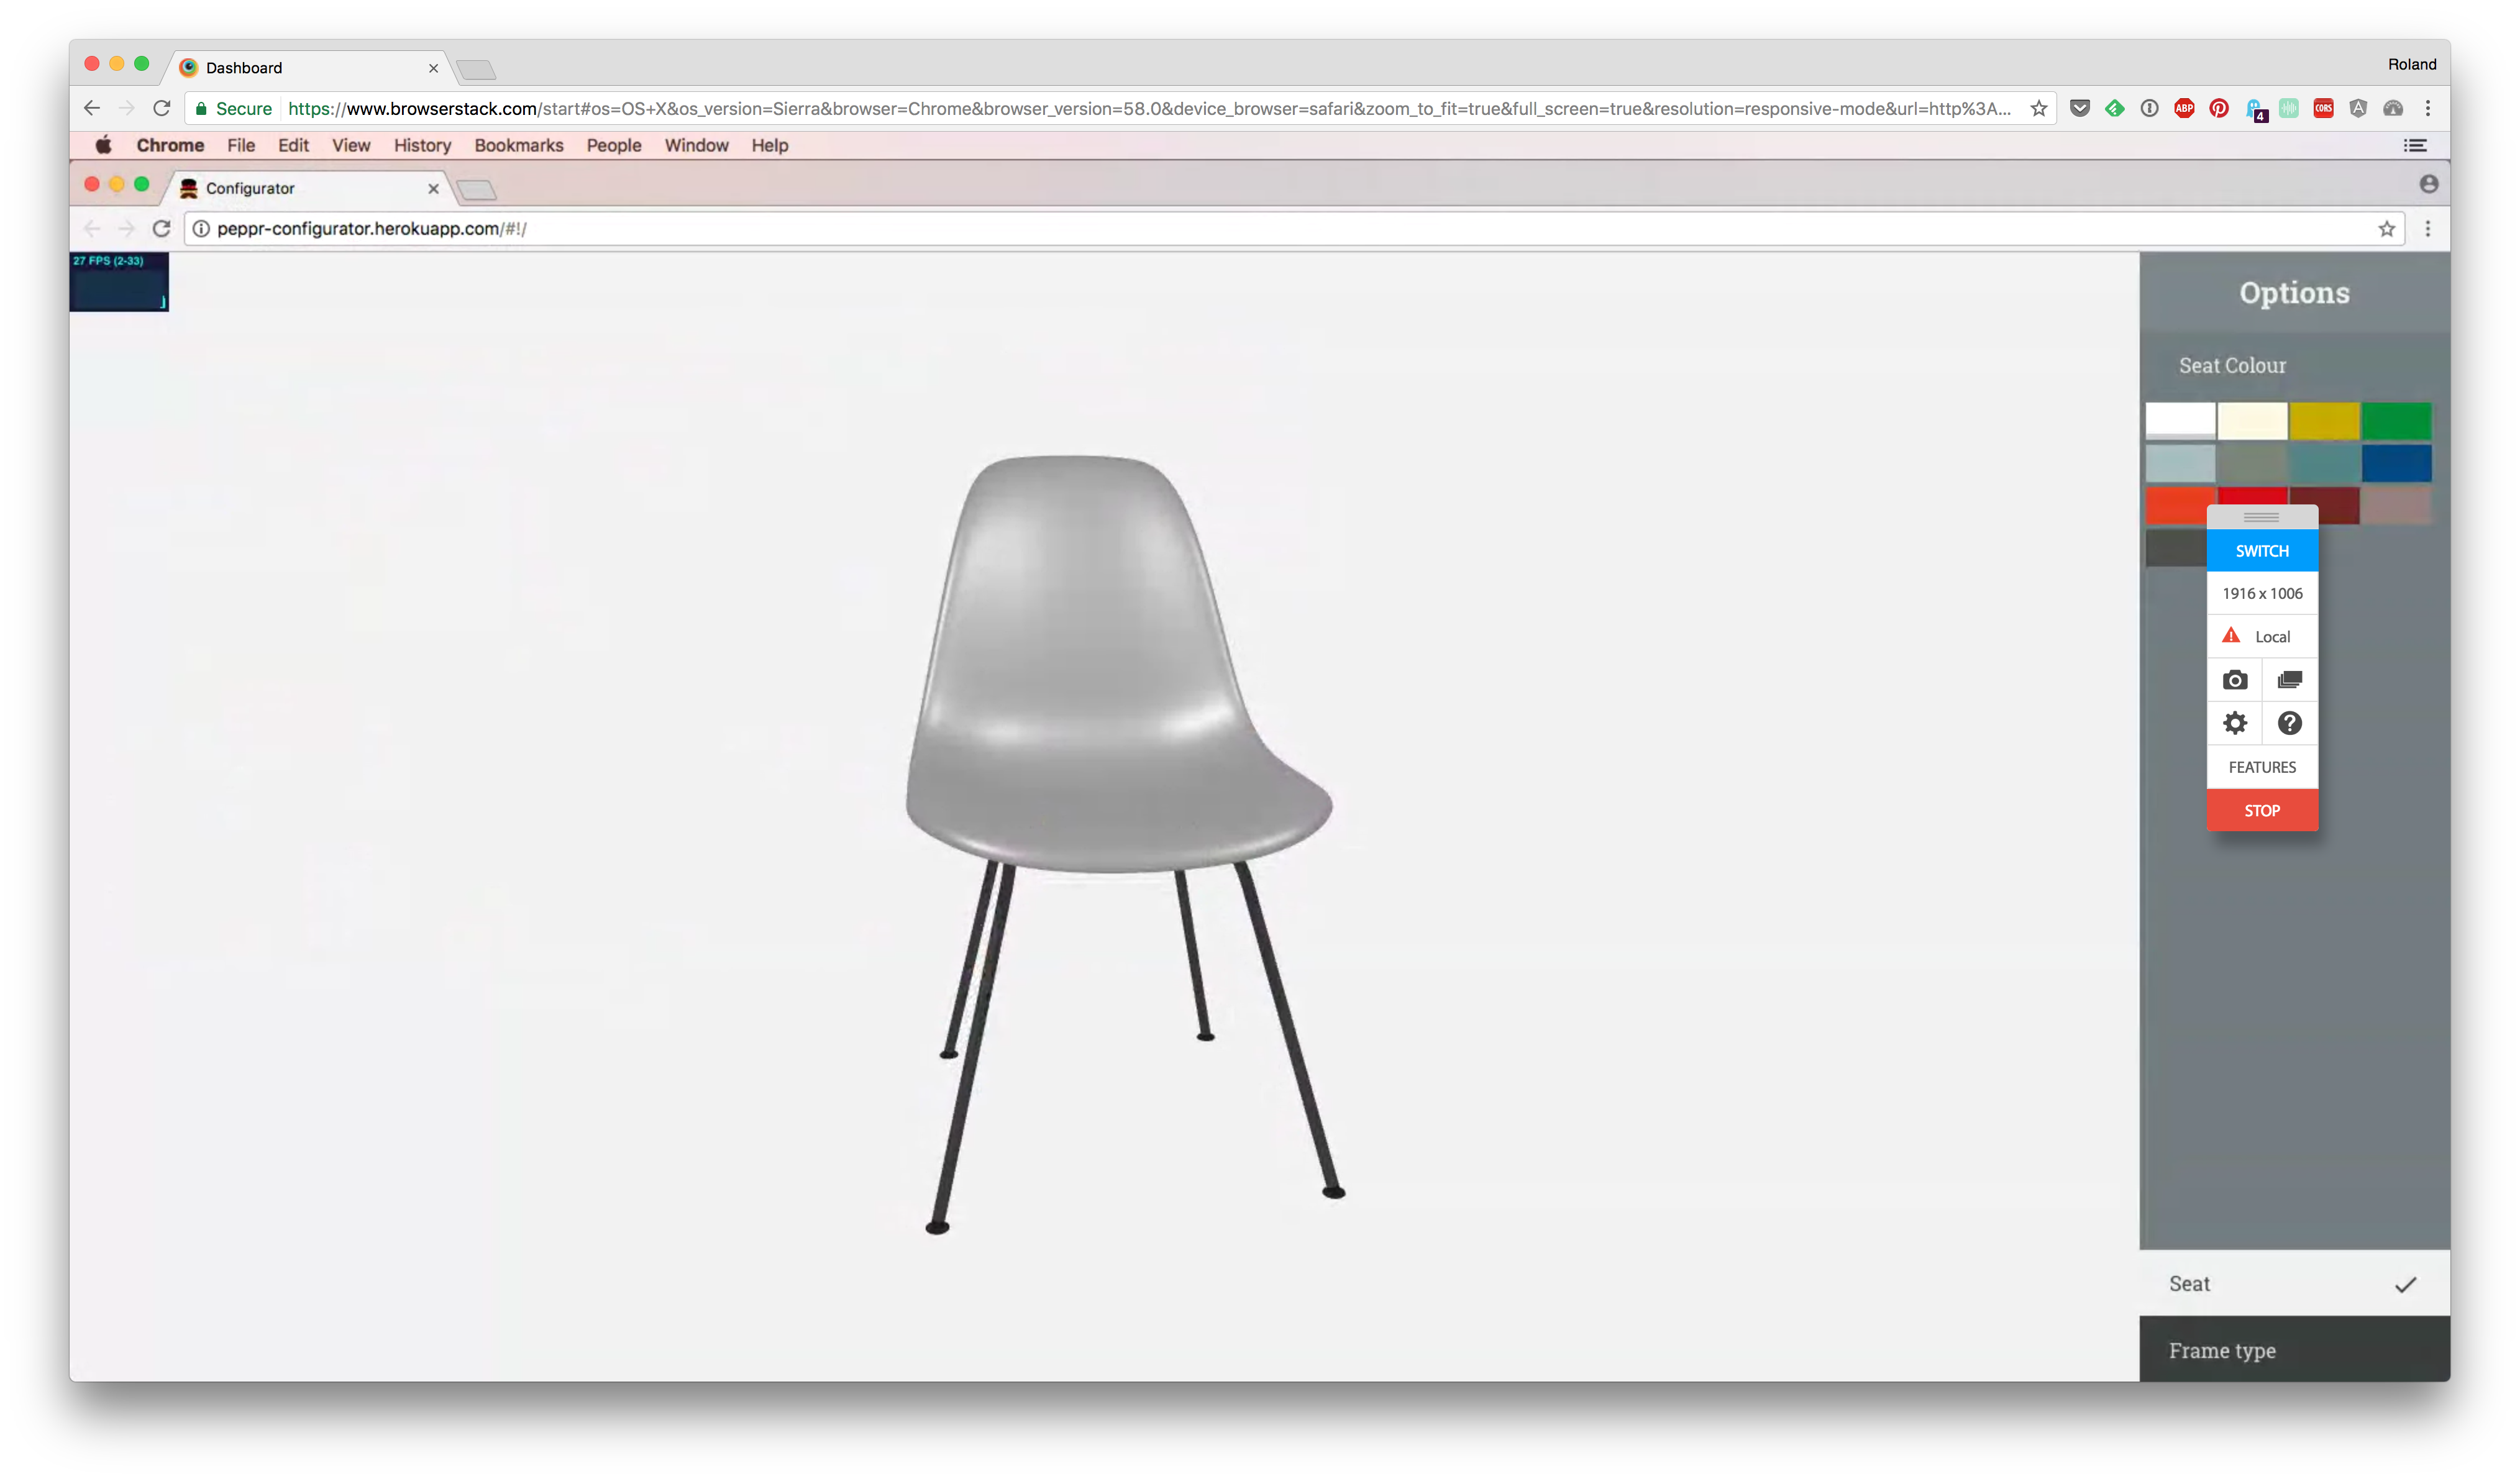
\includegraphics[width=15cm]{images/deviceScreenshots/MacOSChrome}
\caption{Browserstack screenshot: MacOS Chrome}
\label{attachment:MacOSChrome}
\end{figure}

\begin{figure}
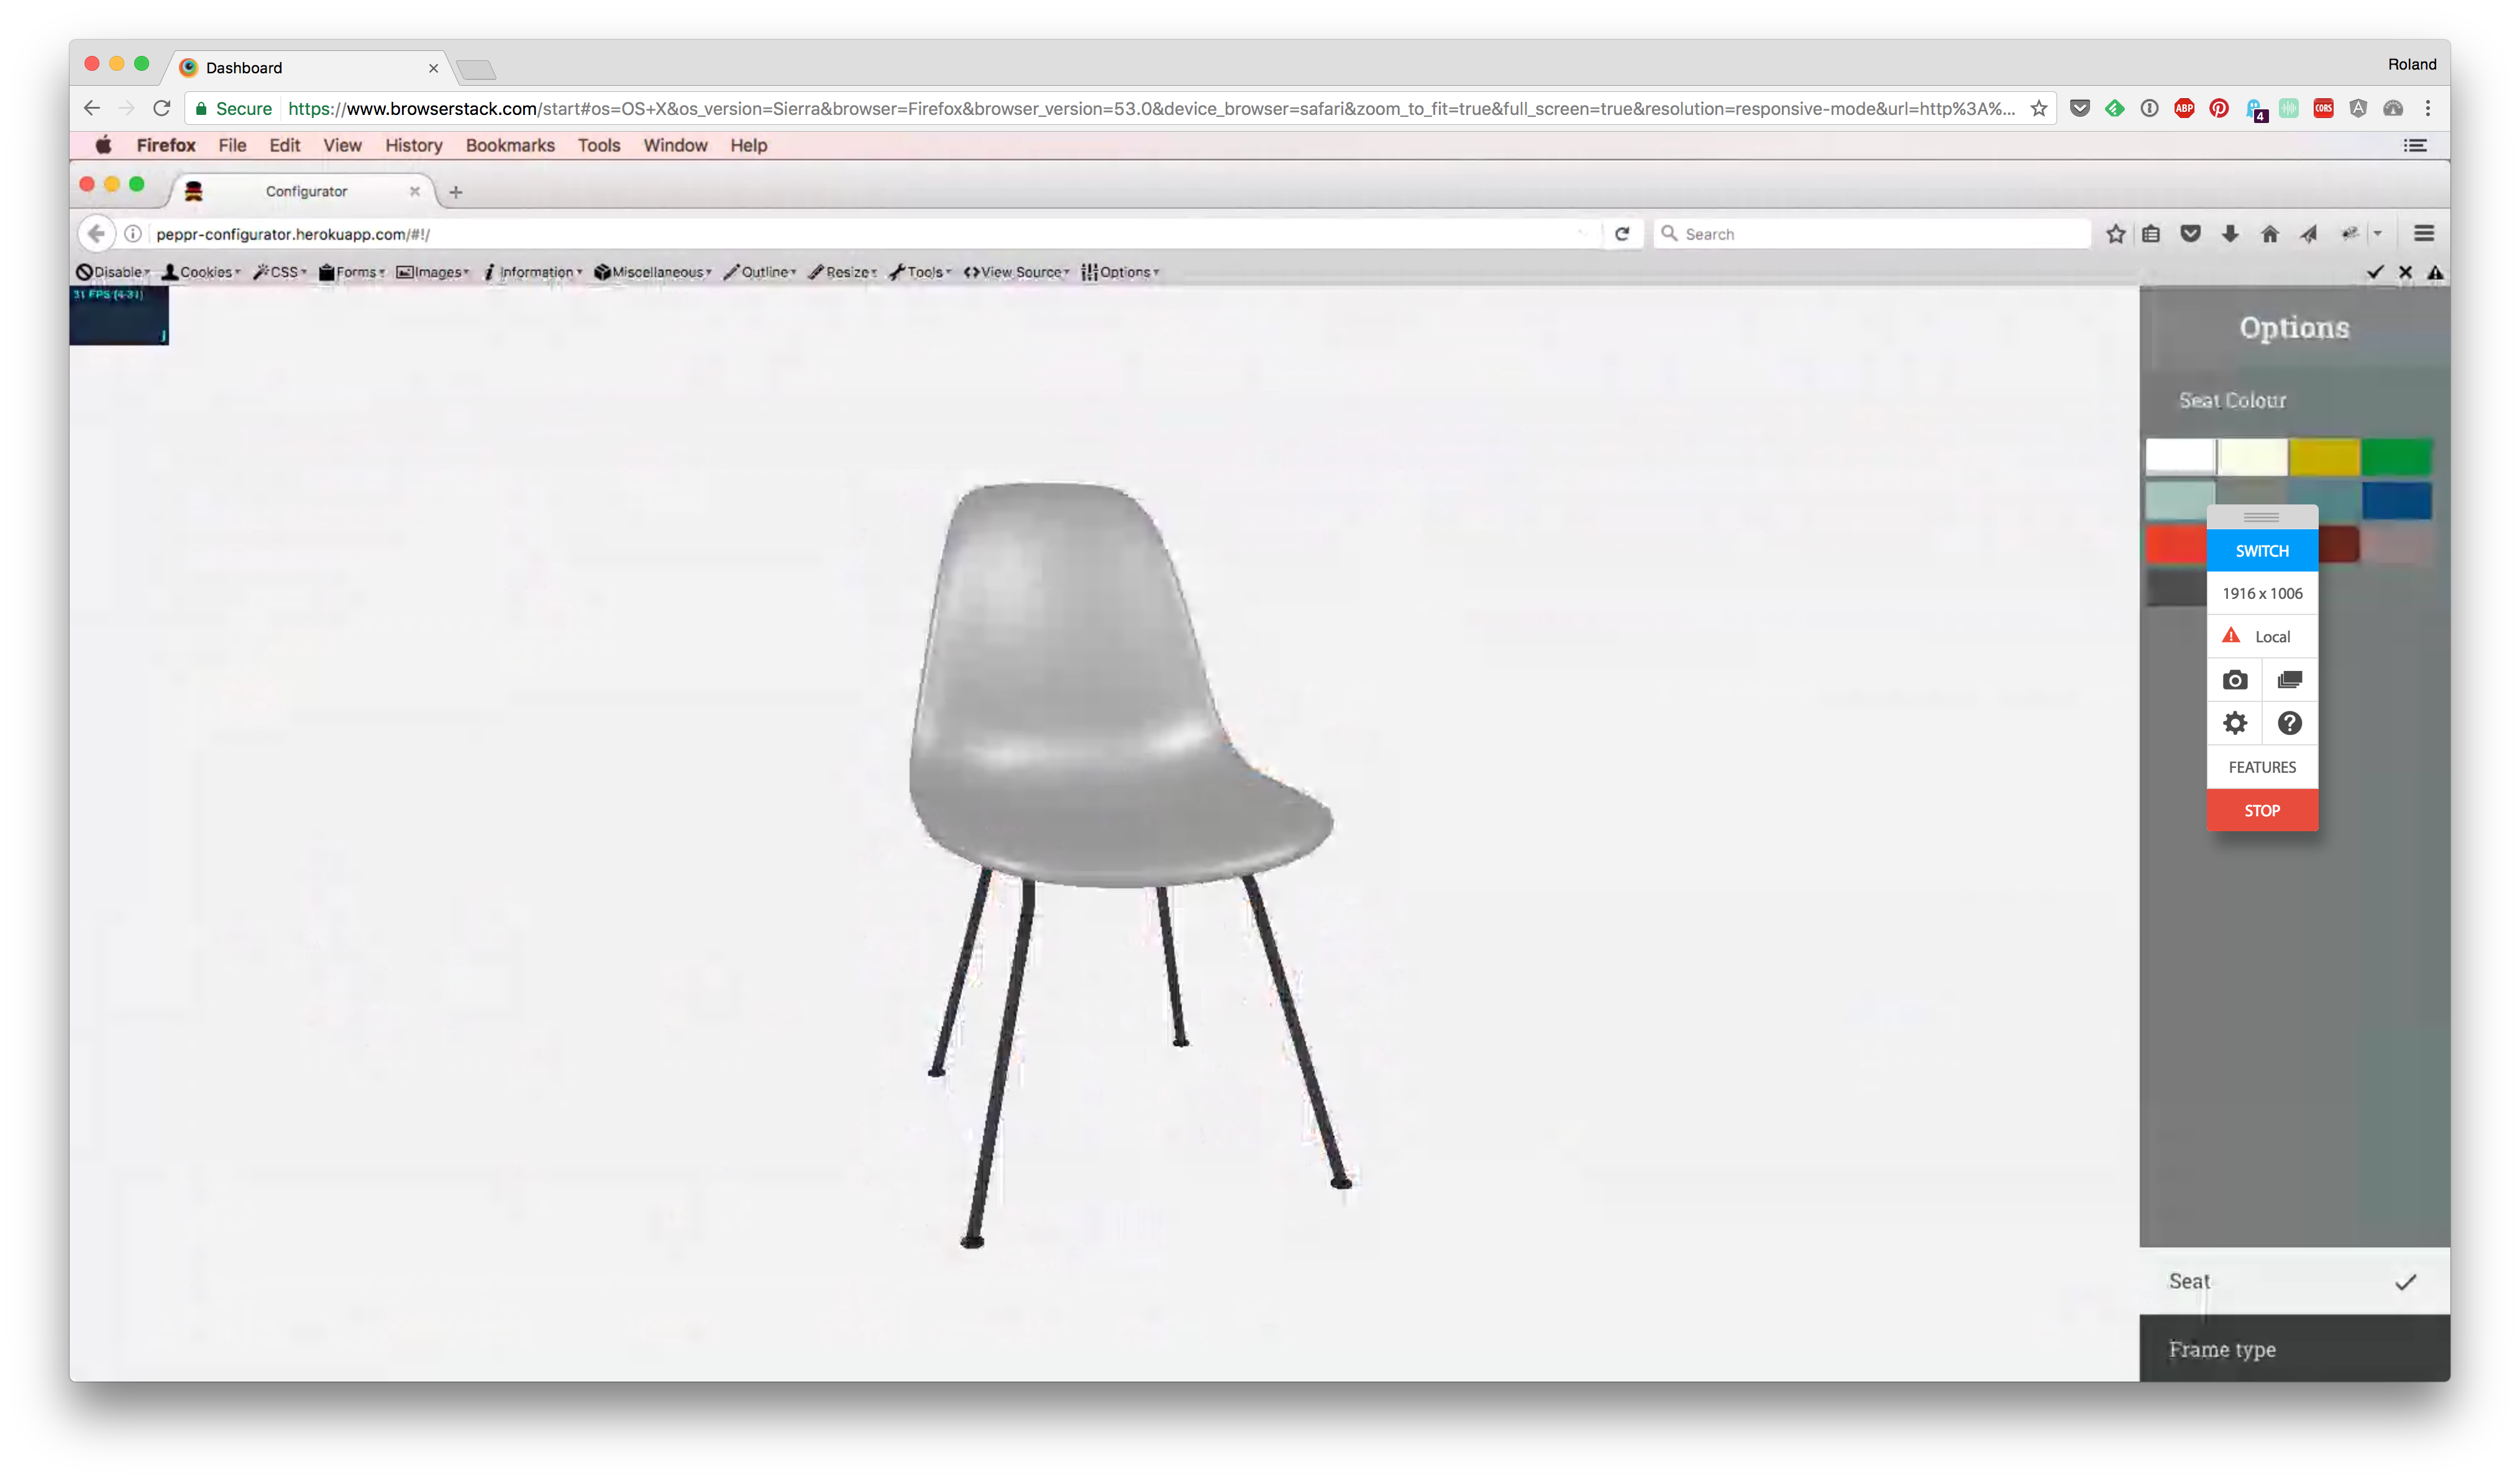
\includegraphics[width=15cm]{images/deviceScreenshots/MacOSFirefox}
\caption{Browserstack screenshot: MacOS Firefox}
\label{attachment:MacOSFirefox}
\end{figure}

\clearpage

\begin{figure}
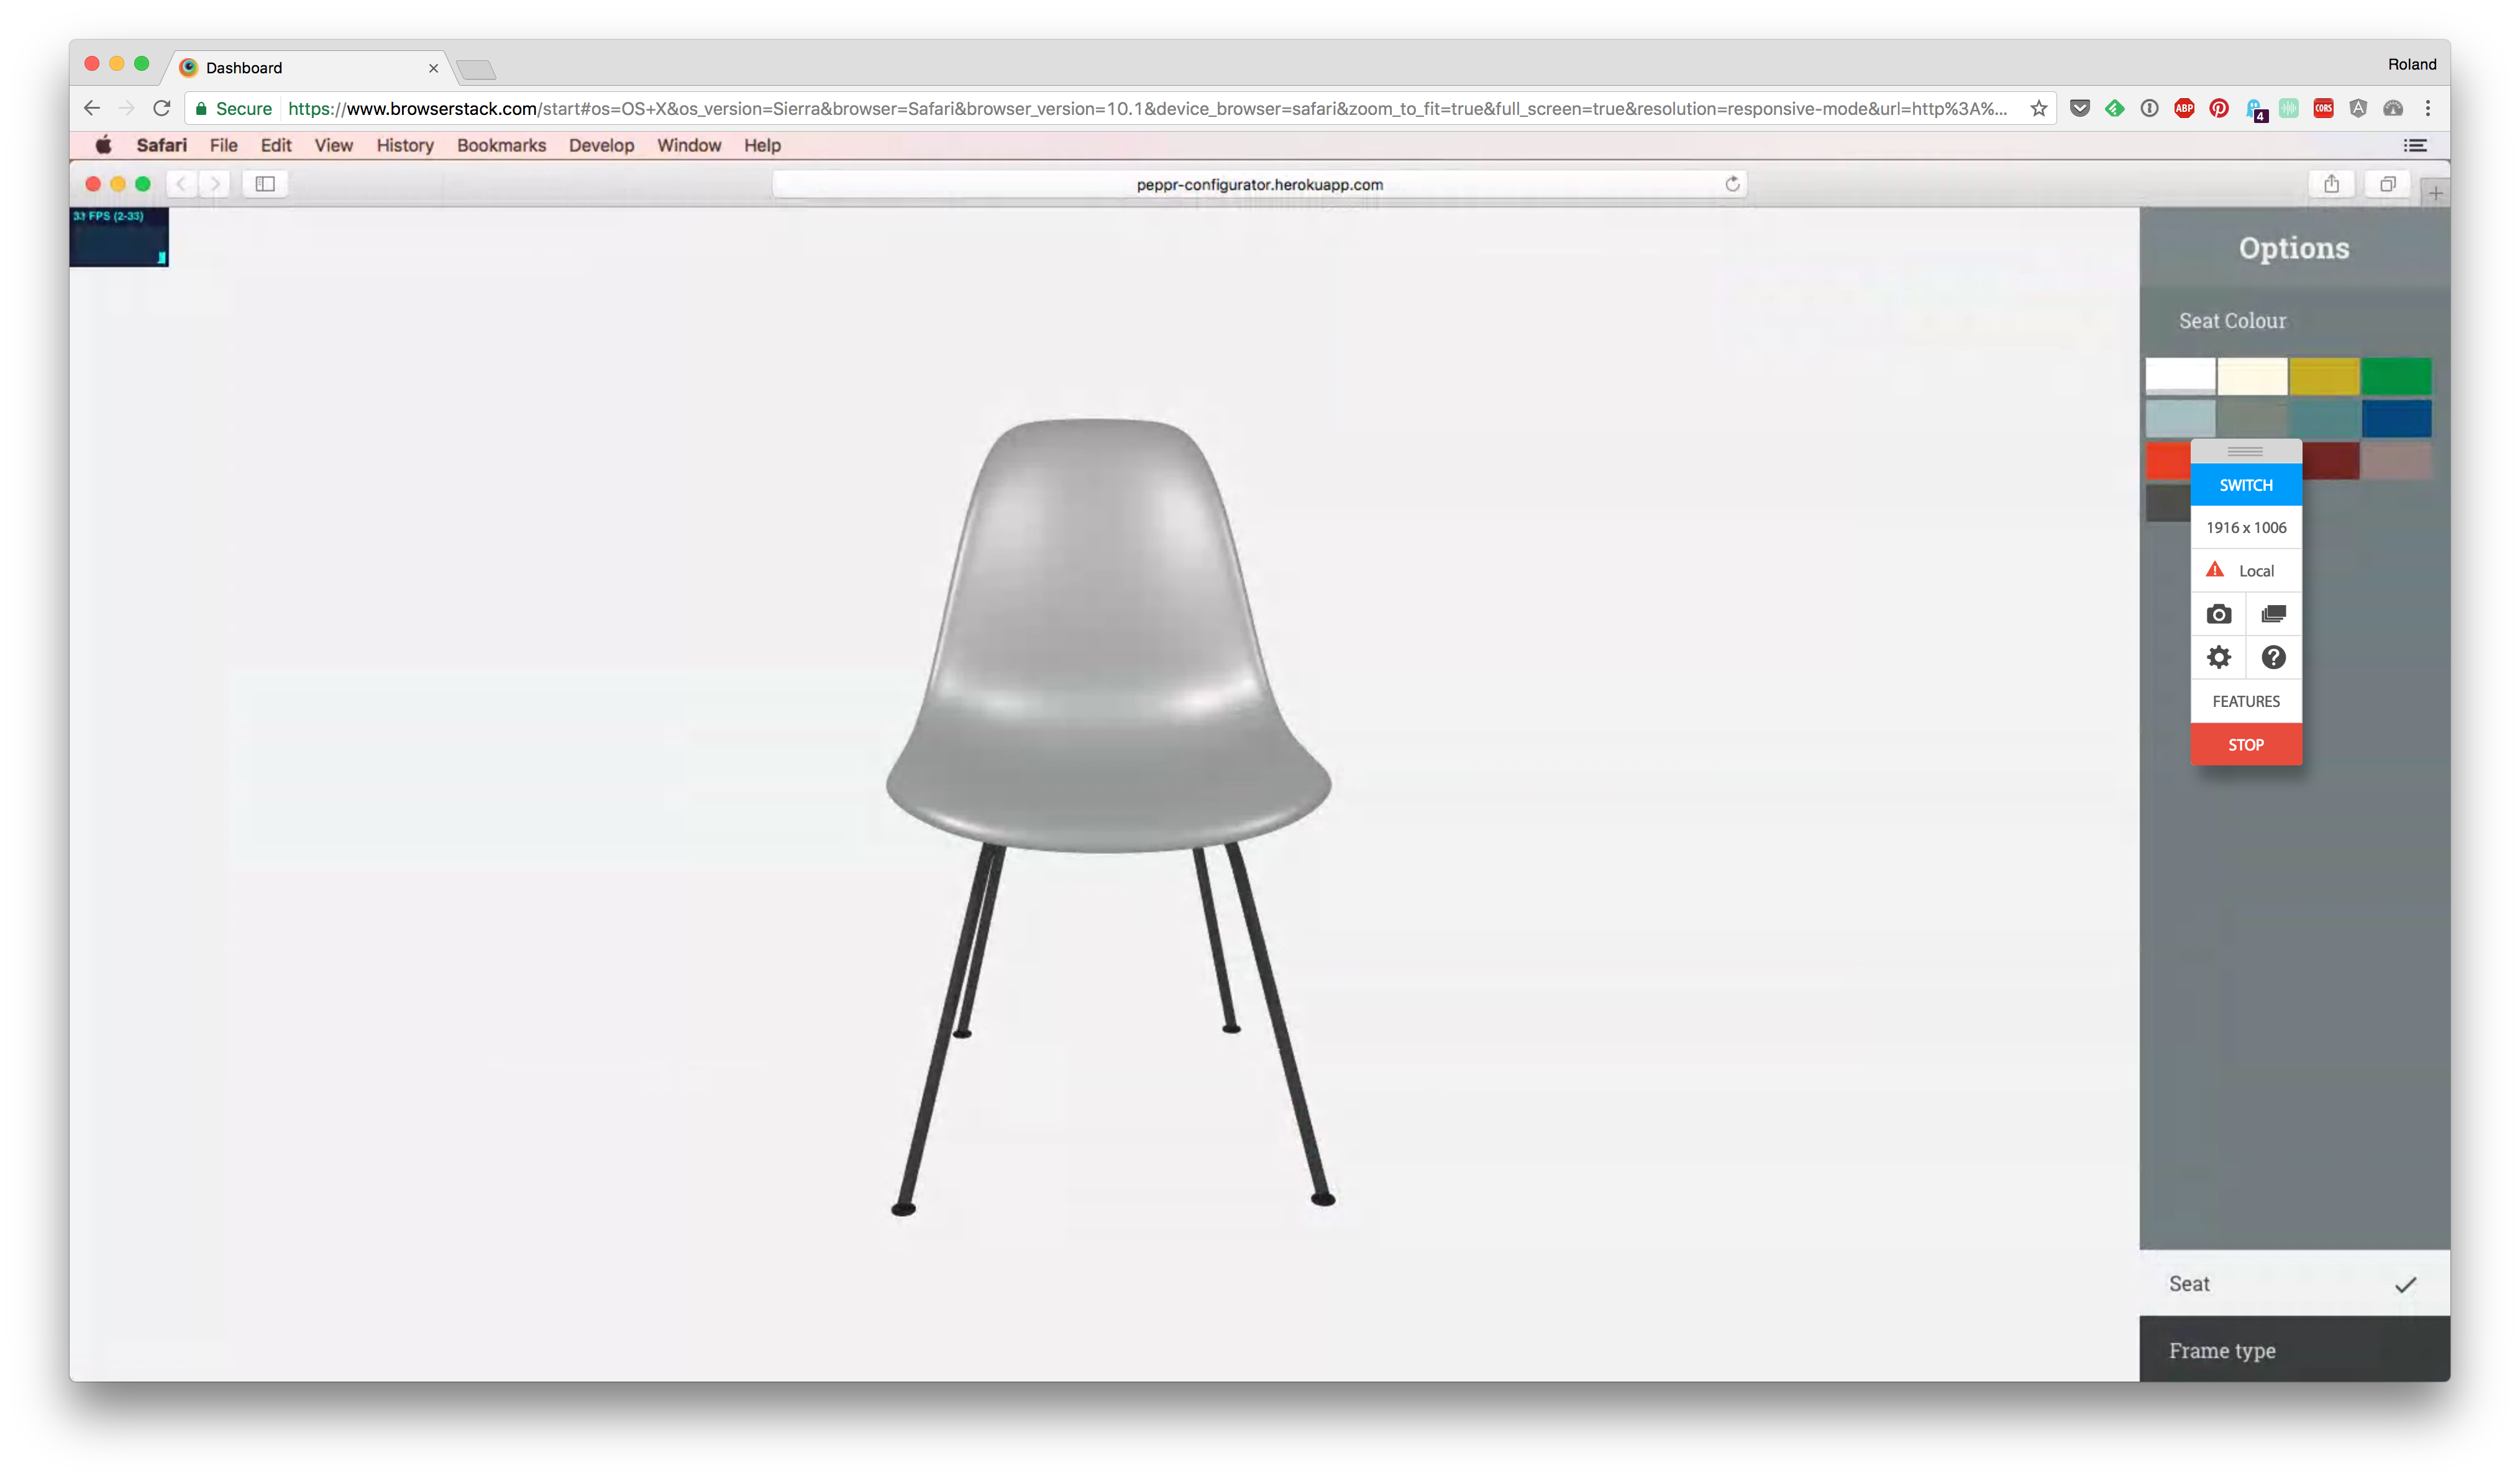
\includegraphics[width=15cm]{images/deviceScreenshots/MacOSSafari}
\caption{Browserstack screenshot: MacOS Safari}
\label{attachment:MacOSSafari}
\end{figure}

\begin{figure}
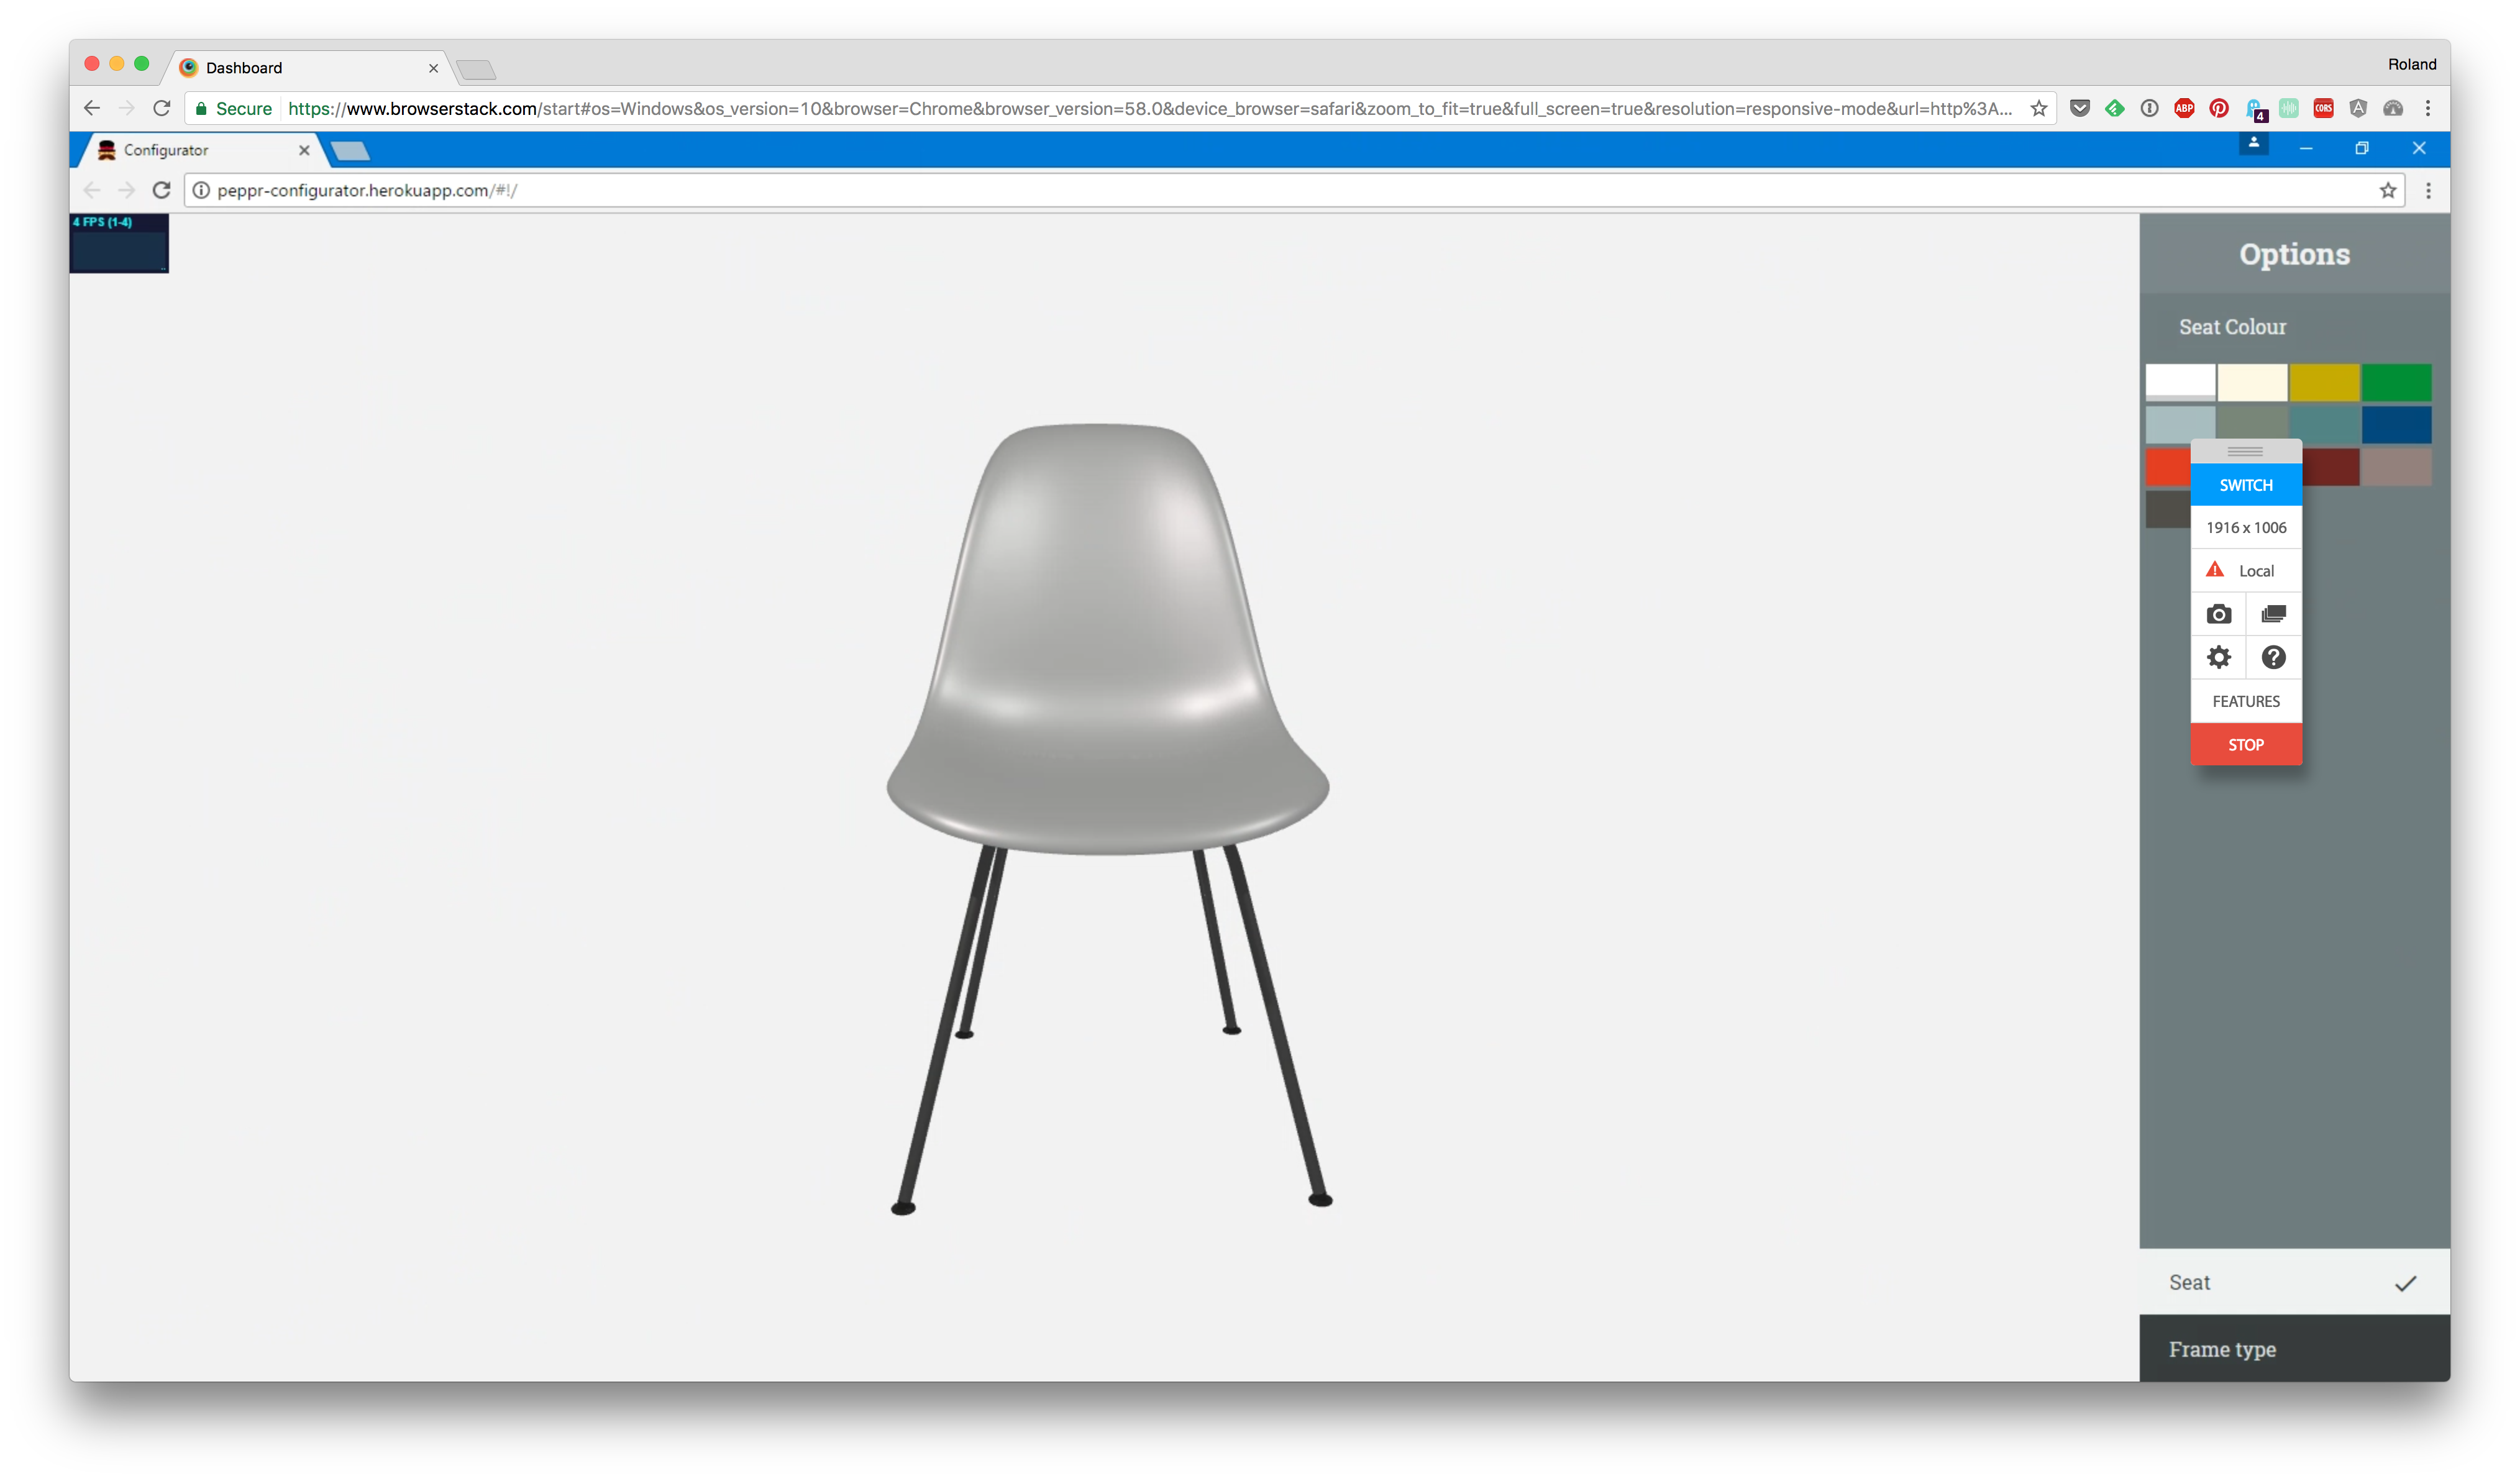
\includegraphics[width=15cm]{images/deviceScreenshots/Windows10Chrome}
\caption{Browserstack screenshot: Windows 10 Chrome}
\label{attachment:Windows10Chrome}
\end{figure}

\clearpage

\begin{figure}
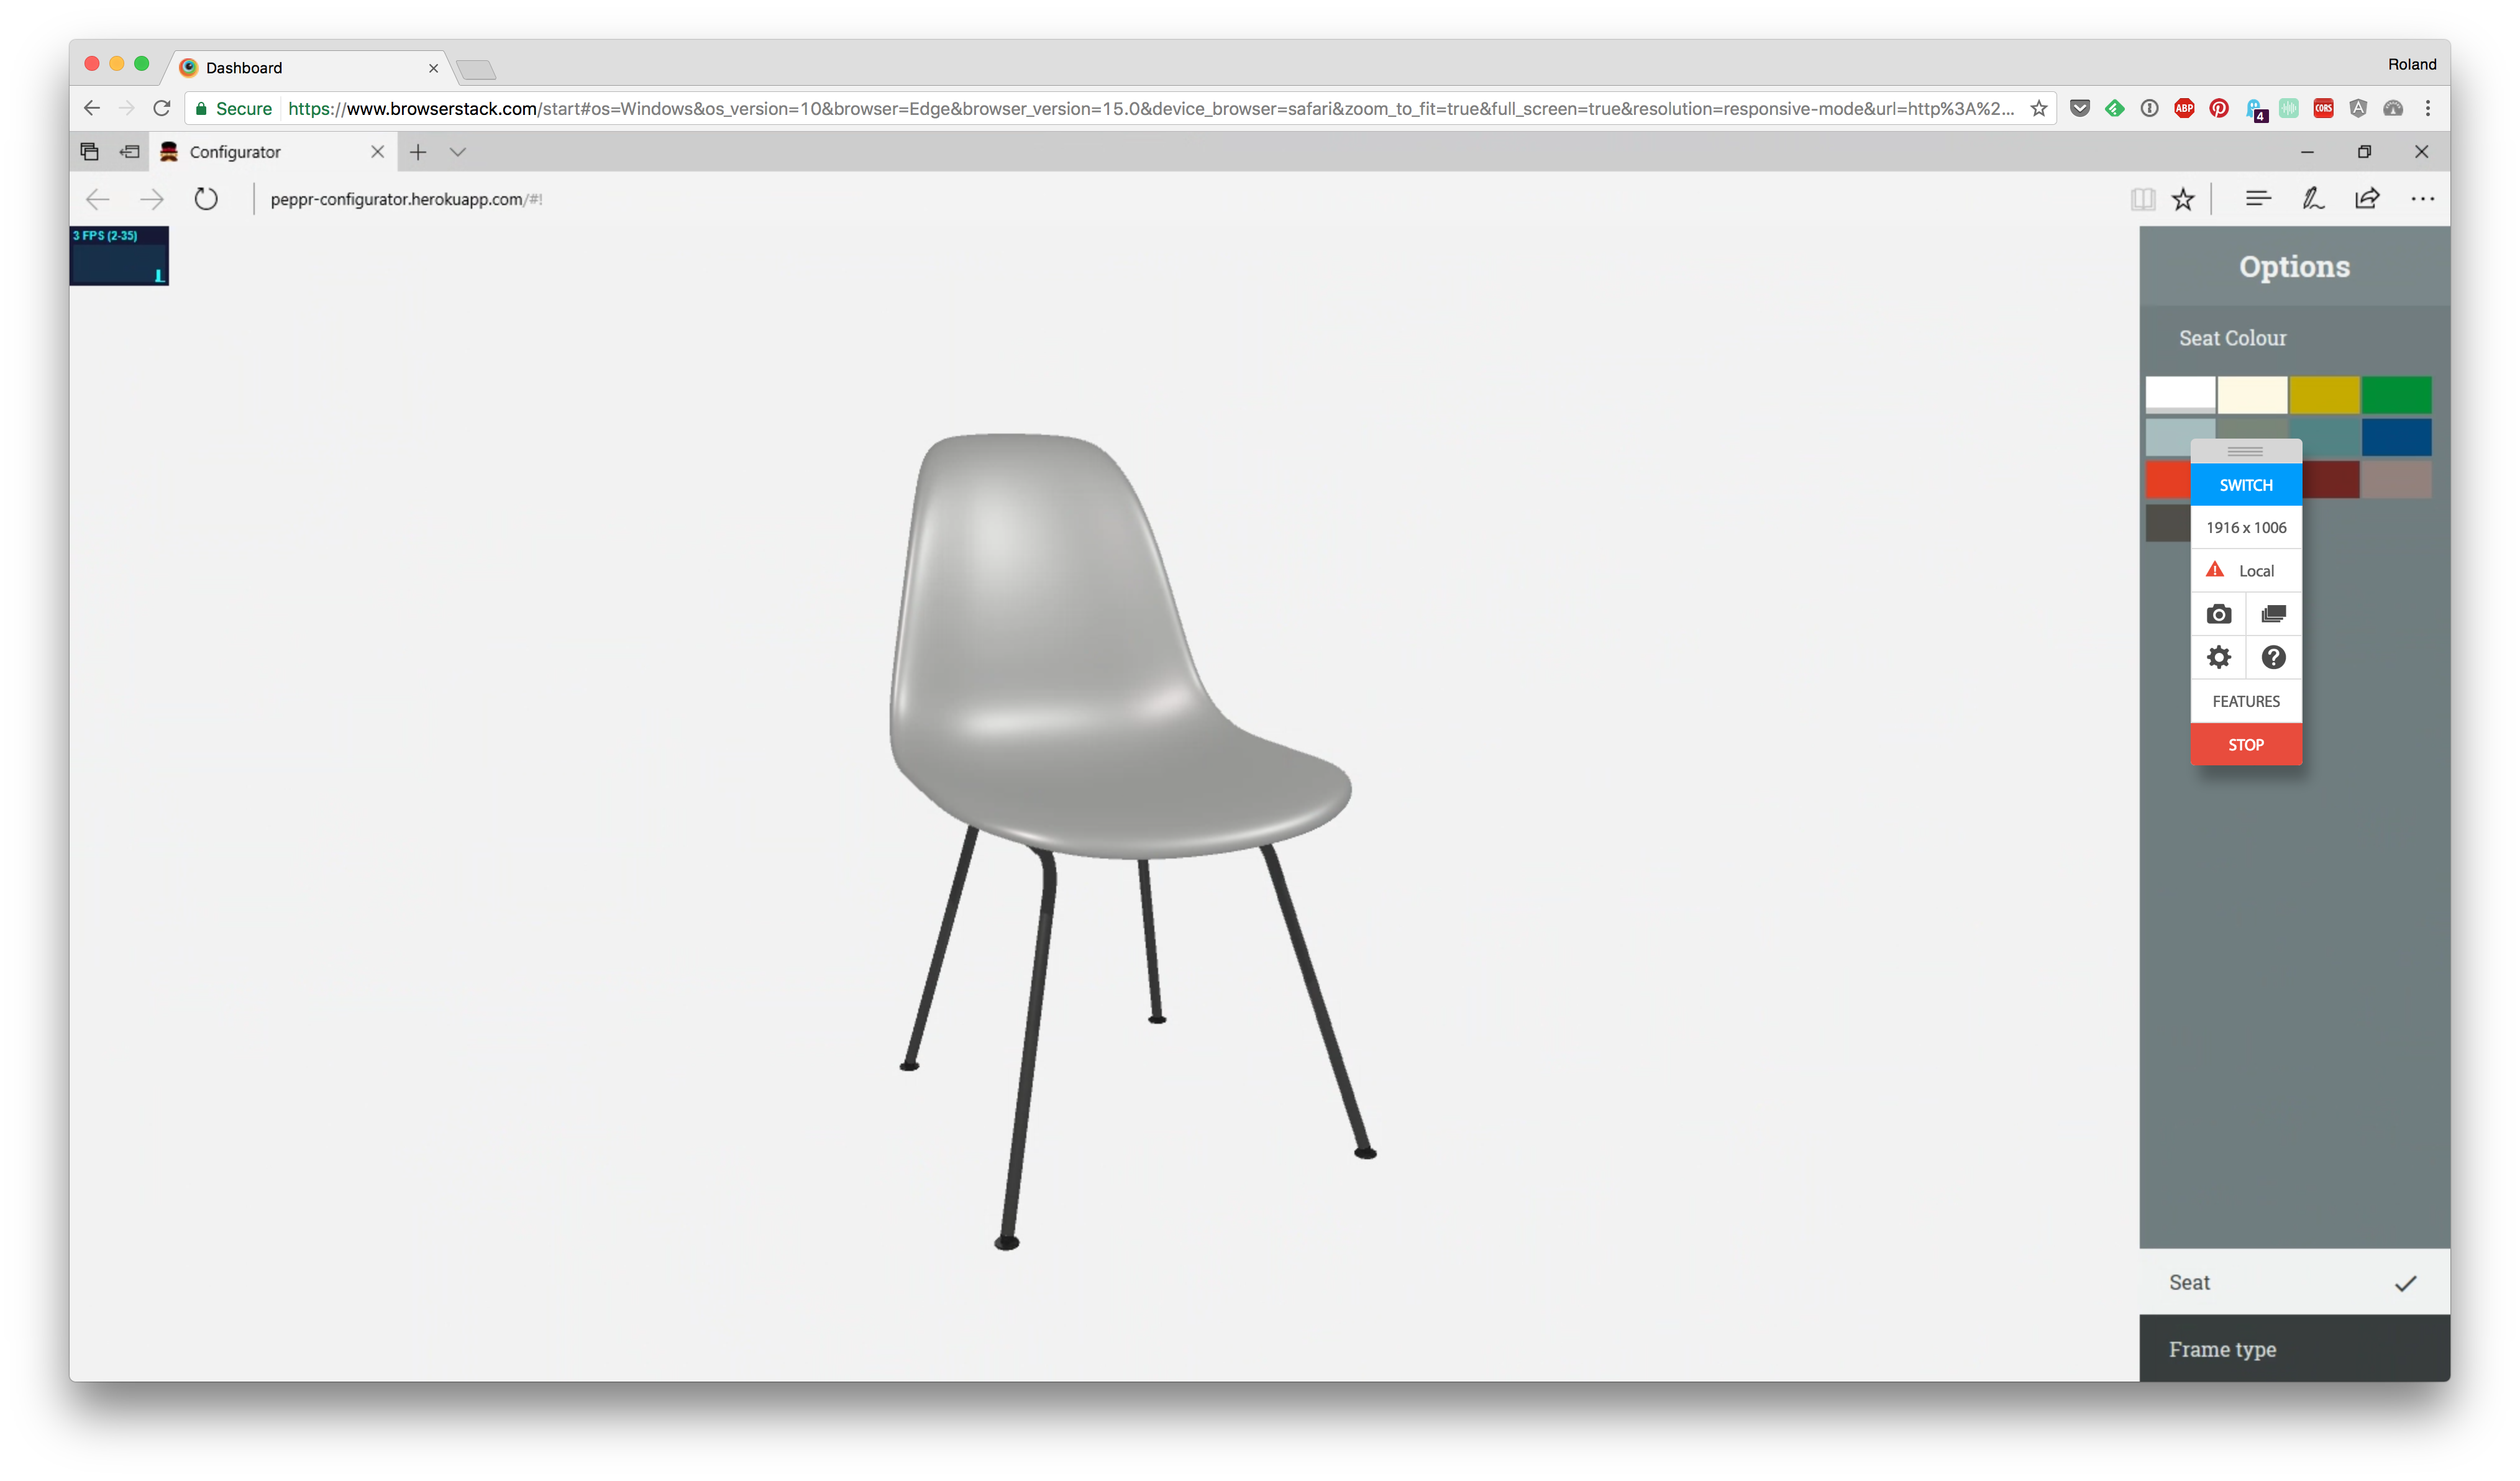
\includegraphics[width=15cm]{images/deviceScreenshots/Windows10Edge}
\caption{Browserstack screenshot: Windows 10 Edge}
\label{attachment:Windows10Edge}
\end{figure}

\begin{figure}
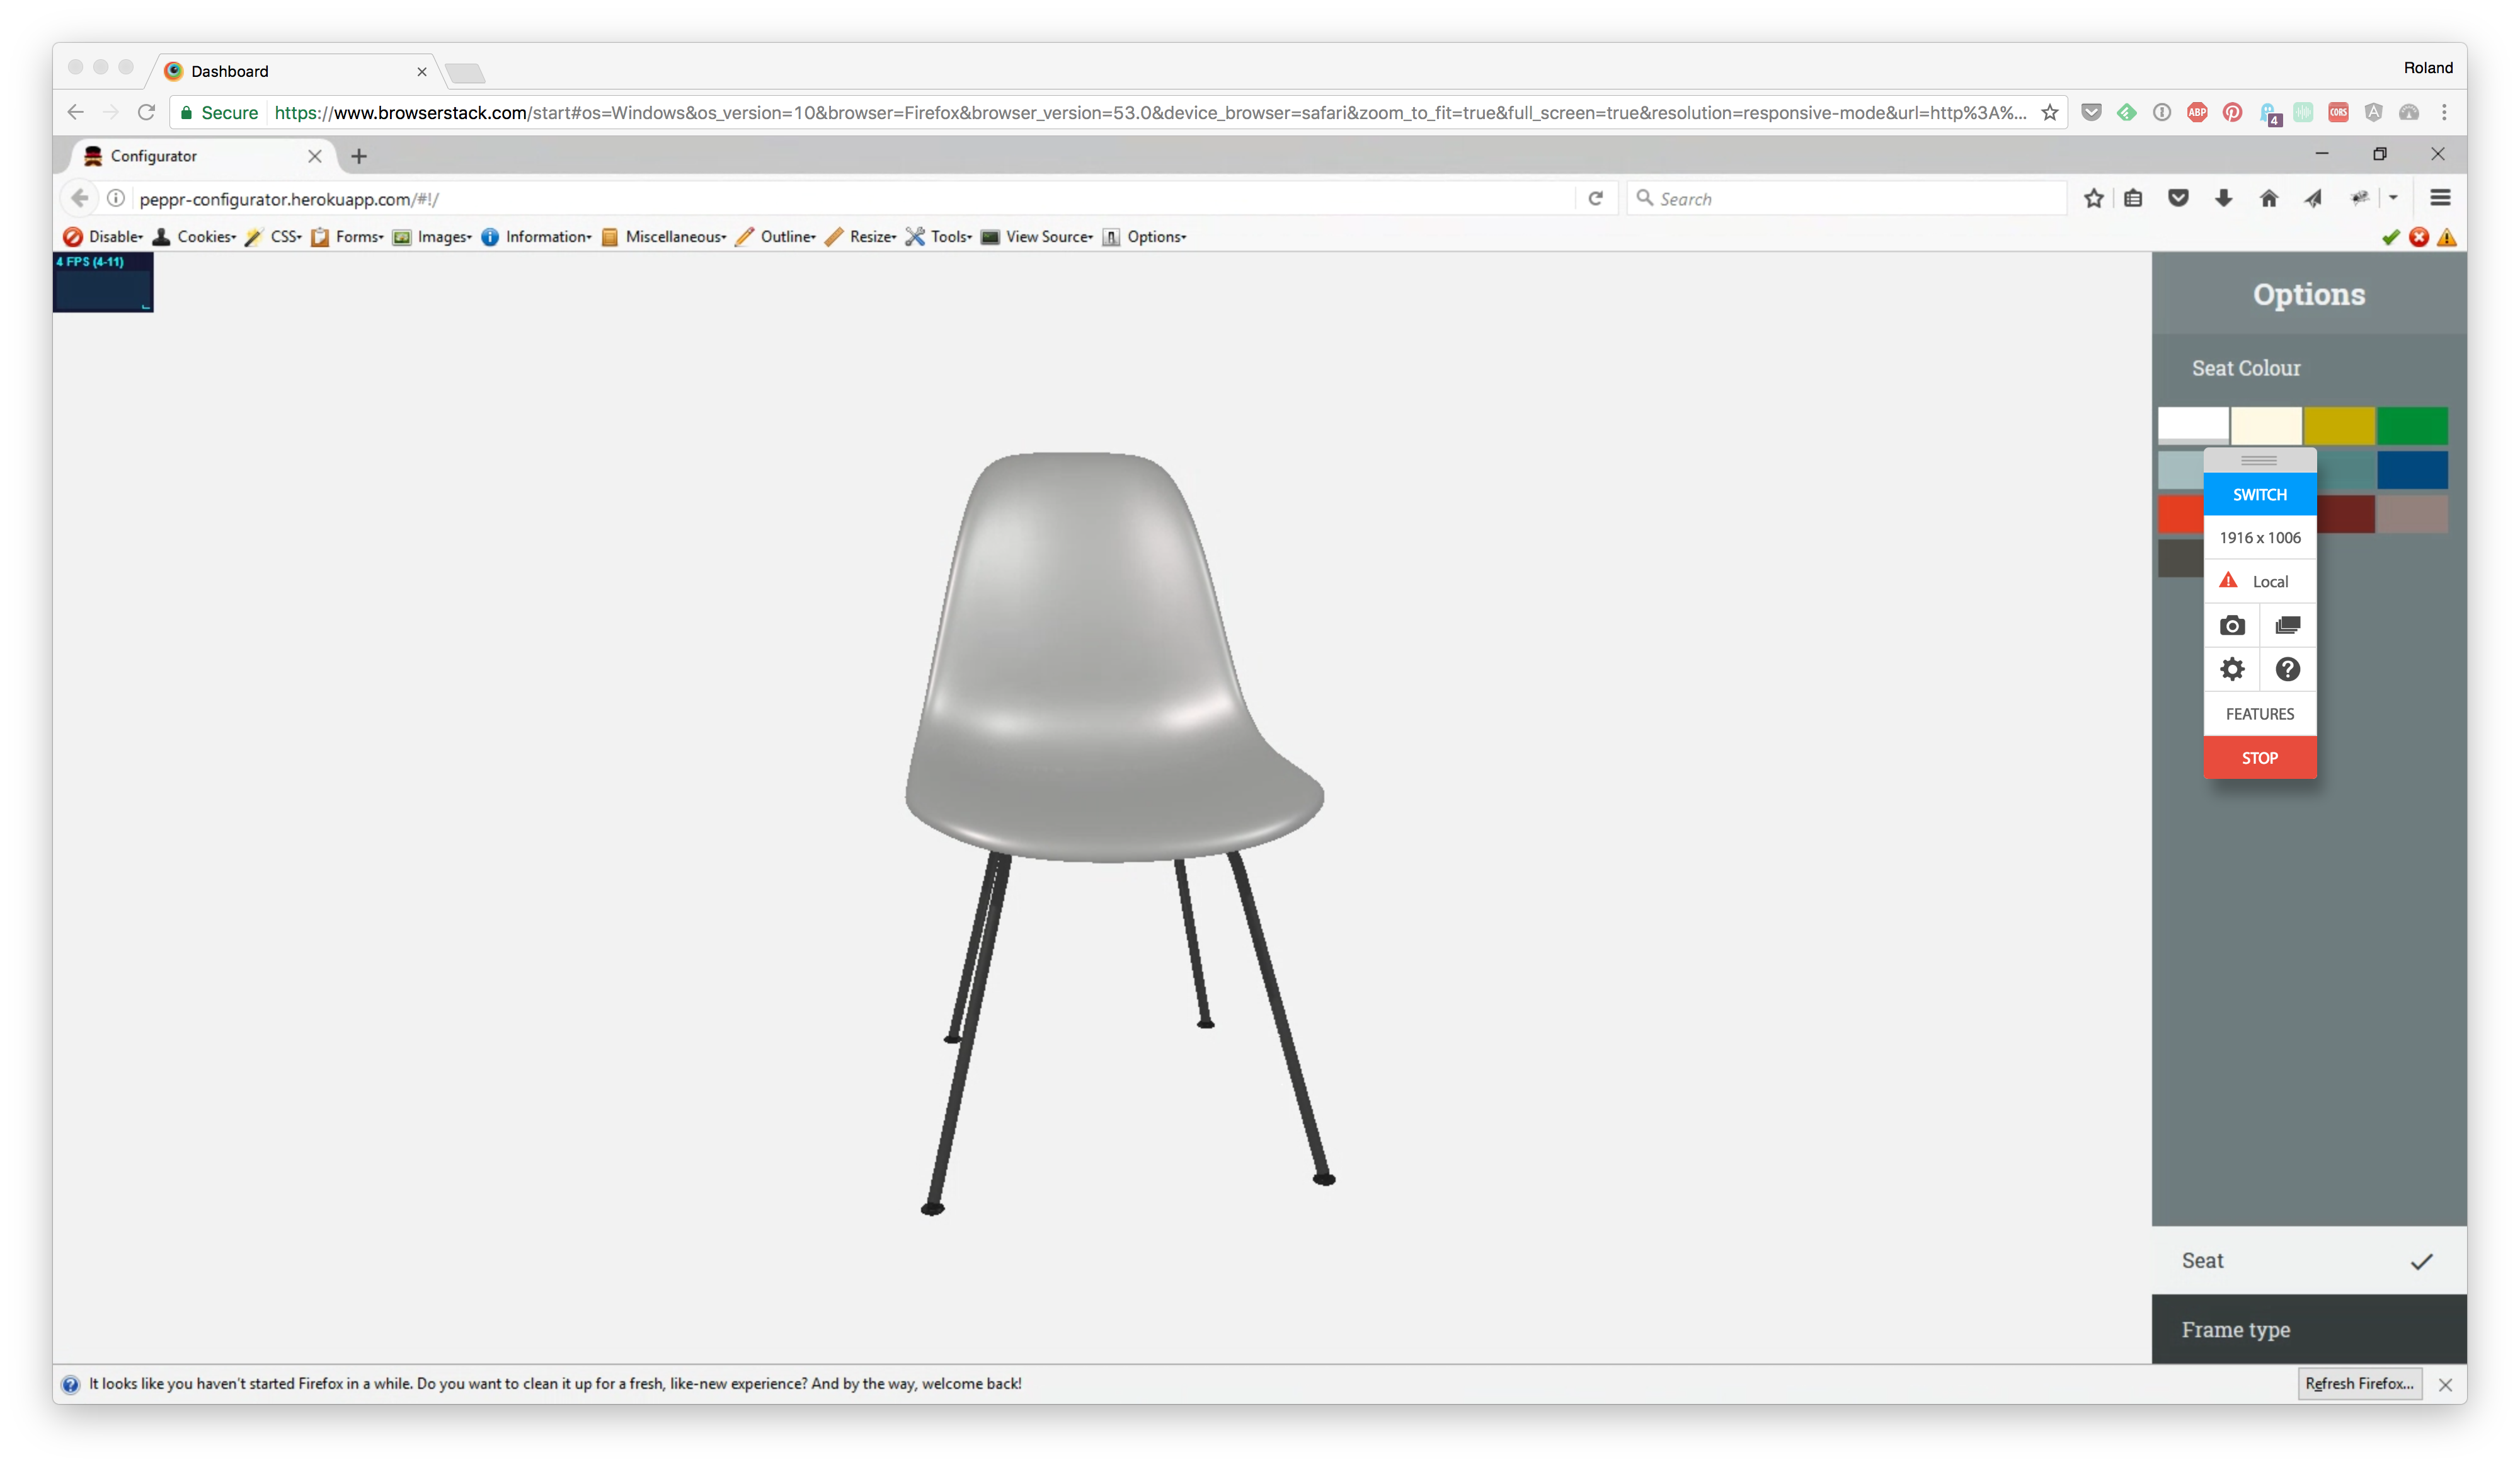
\includegraphics[width=15cm]{images/deviceScreenshots/Windows10Firefox}
\caption{Browserstack screenshot: Windows 10 FireFox}
\label{attachment:Windows10Firefox}
\end{figure}

